% Generated fragments require trusted human review before compilation.
% This binder never requests shell escape or runs external tools.
\documentclass[11pt]{article}
% Trusted shared apparatus. Requires LuaLaTeX; never use shell escape.
\usepackage{fontspec}
\defaultfontfeatures{Ligatures=TeX}
\IfFontExistsTF{Noto Serif}{\setmainfont{Noto Serif}}{%
  \IfFontExistsTF{DejaVu Serif}{\setmainfont{DejaVu Serif}}{%
    \IfFontExistsTF{Times New Roman}{\setmainfont{Times New Roman}}{%
      \PackageError{gelfand-binder}{No configured Cyrillic serif font installed}{Install Noto Serif or DejaVu Serif, or select an installed Cyrillic font.}%
    }%
  }%
}
\IfFontExistsTF{Noto Sans}{\setsansfont{Noto Sans}}{%
  \IfFontExistsTF{DejaVu Sans}{\setsansfont{DejaVu Sans}}{\setsansfont{Arial}}%
}
\IfFontExistsTF{Noto Sans Mono}{\setmonofont{Noto Sans Mono}}{%
  \IfFontExistsTF{DejaVu Sans Mono}{\setmonofont{DejaVu Sans Mono}}{\setmonofont{Courier New}}%
}
\usepackage[a4paper,margin=22mm]{geometry}
\usepackage{amsmath,amssymb,amsthm,mathtools}
\usepackage{xcolor}
\usepackage{tikz}
\usepackage{tikz-cd}
\usetikzlibrary{arrows.meta,positioning,calc}
\usepackage{hyperref}
\hypersetup{unicode=true,colorlinks=true,linkcolor=blue,pdftitle={Gelfand transcription binder}}
\newtheorem{theorem}{Theorem}
\newtheorem{lemma}{Lemma}
\newtheorem{proposition}{Proposition}
\newtheorem{corollary}{Corollary}
\theoremstyle{definition}
\newtheorem{definition}{Definition}
\newtheorem{example}{Example}
\theoremstyle{remark}
\newtheorem{remark}{Remark}
\setlength{\parindent}{0pt}
\setlength{\parskip}{0.55em}
\setlength{\emergencystretch}{3em}
\newcommand{\SourcePage}[2]{%
  \clearpage\phantomsection\label{#1:source-page}%
  \addcontentsline{toc}{subsection}{#1}%
  {\small\sffamily\color{blue!60!black}Source scan frame: #1; visible page/leaf label: #2}\par\medskip%
}
\newcommand{\Unclear}[3]{%
  \begingroup\color{orange!70!black}%
  [Unresolved reading #1/#2: #3]\endgroup%
}
\newcommand{\Incomplete}[3]{%
  \par\begingroup\color{red!65!black}\textbf{Incomplete #1/#2:} #3\endgroup\par%
}
\newcommand{\SourceFigure}[3]{%
  \par\begingroup\color{blue!60!black}\textbf{\hyperref[#1:source-page]{Source figure #1/#2}:} #3%
  \par\textit{Consult the authoritative scan at this locator.}\endgroup\par%
}



% Reader layout only. Original diplomatic text is retained verbatim.
\setlength{\parskip}{0.35em}
\setlength{\emergencystretch}{4em}
\renewcommand{\SourcePage}[2]{%
  \par\addvspace{1em}\phantomsection\label{#1:source-page}%
  \addcontentsline{toc}{subsection}{#1}%
  {\footnotesize\sffamily\color{blue!55!black}#1%
    \def\givenlabel{#2}\def\nolabel{unlabelled}%
    \ifx\givenlabel\nolabel\else\quad[номер в источнике: #2]\fi
  }\par\nobreak\smallskip%
}
\renewcommand{\Unclear}[3]{%
  \begingroup\color{orange!65!black}%
  \ifmmode\text{[неясно: #3]}\else[неясно: #3]\fi\endgroup%
}
\renewcommand{\Incomplete}[3]{%
  \par\begingroup\color{red!60!black}\textbf{Неразобранный фрагмент:} #3%
  \endgroup\par%
}
\renewcommand{\SourceFigure}[3]{%
  \par\begingroup\color{blue!55!black}\textbf{Рисунок:} #3%
  \par{\small\textit{Исходный рисунок: \hyperref[#1:source-page]{#1}, #2.}}%
  \endgroup\par%
}
\hypersetup{pdftitle={Семинар И. М. Гельфанда. Дипломатическая транскрипция},pdfauthor={},pdfsubject={Русское рабочее издание с отмеченными сомнительными чтениями}}

\usepackage[normalem]{ulem}
\usepackage{newunicodechar}
\usepackage{adjustbox}
\newfontfamily\SourceSymbolFont{Segoe UI Symbol}
\newfontfamily\SourceCJKFont{MS Gothic}
\let\DiplomaticMathUnderline\underline
\renewcommand{\underline}[1]{\ifmmode\DiplomaticMathUnderline{#1}\else\uline{#1}\fi}
\newunicodechar{→}{\ifmmode\text{{\SourceSymbolFont\char"2192}}\else{\SourceSymbolFont\char"2192}\fi}
\newunicodechar{⇒}{\ifmmode\text{{\SourceSymbolFont\char"21D2}}\else{\SourceSymbolFont\char"21D2}\fi}
\newunicodechar{∀}{\ifmmode\text{{\SourceSymbolFont\char"2200}}\else{\SourceSymbolFont\char"2200}\fi}
\newunicodechar{∂}{\ifmmode\text{{\SourceSymbolFont\char"2202}}\else{\SourceSymbolFont\char"2202}\fi}
\newunicodechar{∈}{\ifmmode\text{{\SourceSymbolFont\char"2208}}\else{\SourceSymbolFont\char"2208}\fi}
\newunicodechar{∌}{\ifmmode\text{{\SourceSymbolFont\char"220C}}\else{\SourceSymbolFont\char"220C}\fi}
\newunicodechar{√}{\ifmmode\text{{\SourceSymbolFont\char"221A}}\else{\SourceSymbolFont\char"221A}\fi}
\newunicodechar{∞}{\ifmmode\text{{\SourceSymbolFont\char"221E}}\else{\SourceSymbolFont\char"221E}\fi}
\newunicodechar{∧}{\ifmmode\text{{\SourceSymbolFont\char"2227}}\else{\SourceSymbolFont\char"2227}\fi}
\newunicodechar{∩}{\ifmmode\text{{\SourceSymbolFont\char"2229}}\else{\SourceSymbolFont\char"2229}\fi}
\newunicodechar{∪}{\ifmmode\text{{\SourceSymbolFont\char"222A}}\else{\SourceSymbolFont\char"222A}\fi}
\newunicodechar{∫}{\ifmmode\text{{\SourceSymbolFont\char"222B}}\else{\SourceSymbolFont\char"222B}\fi}
\newunicodechar{∴}{\ifmmode\text{{\SourceSymbolFont\char"2234}}\else{\SourceSymbolFont\char"2234}\fi}
\newunicodechar{∼}{\ifmmode\text{{\SourceSymbolFont\char"223C}}\else{\SourceSymbolFont\char"223C}\fi}
\newunicodechar{≈}{\ifmmode\text{{\SourceSymbolFont\char"2248}}\else{\SourceSymbolFont\char"2248}\fi}
\newunicodechar{≠}{\ifmmode\text{{\SourceSymbolFont\char"2260}}\else{\SourceSymbolFont\char"2260}\fi}
\newunicodechar{≤}{\ifmmode\text{{\SourceSymbolFont\char"2264}}\else{\SourceSymbolFont\char"2264}\fi}
\newunicodechar{≥}{\ifmmode\text{{\SourceSymbolFont\char"2265}}\else{\SourceSymbolFont\char"2265}\fi}
\newunicodechar{⊕}{\ifmmode\text{{\SourceSymbolFont\char"2295}}\else{\SourceSymbolFont\char"2295}\fi}
\newunicodechar{⊗}{\ifmmode\text{{\SourceSymbolFont\char"2297}}\else{\SourceSymbolFont\char"2297}\fi}
\newunicodechar{①}{\ifmmode\text{{\SourceSymbolFont\char"2460}}\else{\SourceSymbolFont\char"2460}\fi}
\newunicodechar{②}{\ifmmode\text{{\SourceSymbolFont\char"2461}}\else{\SourceSymbolFont\char"2461}\fi}
\newunicodechar{③}{\ifmmode\text{{\SourceSymbolFont\char"2462}}\else{\SourceSymbolFont\char"2462}\fi}
\newunicodechar{④}{\ifmmode\text{{\SourceSymbolFont\char"2463}}\else{\SourceSymbolFont\char"2463}\fi}
\newunicodechar{Ⓗ}{\ifmmode\text{{\SourceSymbolFont\char"24BD}}\else{\SourceSymbolFont\char"24BD}\fi}
\newunicodechar{〃}{\ifmmode\text{{\SourceCJKFont\char"3003}}\else{\SourceCJKFont\char"3003}\fi}


% Reader revision 3. Annotation wording and candidates remain unchanged.
\usetikzlibrary{shapes.geometric,decorations.pathreplacing,decorations.markings,patterns,fit}
\newsavebox{\ReaderAnnotationBox}
\newcommand{\ReaderAnnotation}[1]{%
  \sbox{\ReaderAnnotationBox}{[неясно: #1]}%
  \ifdim\wd\ReaderAnnotationBox>.70\linewidth
    \parbox[t]{.70\linewidth}{\raggedright[неясно: #1]}%
  \else\usebox{\ReaderAnnotationBox}\fi%
}
\ExplSyntaxOn
\cs_new_protected:Npn \reader_unclear_candidate:n #1
 {
  \tl_set:Nx \l_tmpa_tl { \tl_to_str:n {#1} }
  % Text explicitly guarded inside a mathematical candidate remains math-safe.
  \regex_replace_all:nnN { \\(?:text|textrm|textnormal|textbf|operatorname)\s*\{[^{}]*\} } { } \l_tmpa_tl
  \regex_match:nVTF { [\x{0400}-\x{052F}] | \$ } \l_tmpa_tl
   { \ifmmode \text{\ReaderAnnotation{#1}} \else \ReaderAnnotation{#1} \fi }
   {
    \ifmmode
      [\text{неясно:~}#1]
    \else
      \regex_match:nVTF { [_^] | \\ } \l_tmpa_tl
       { \ensuremath{[\text{неясно:~}#1]} }
       { \ReaderAnnotation{#1} }
    \fi
   }
 }
\RenewDocumentCommand \Unclear { m m m }
 { \begingroup\color{orange!65!black}\reader_unclear_candidate:n{#3}\endgroup }
\ExplSyntaxOff
\newsavebox{\ReaderIncompleteBox}
\newcommand{\ReaderIncompleteNote}[1]{%
 \sbox{\ReaderIncompleteBox}{\textbf{Неразобранный фрагмент:} #1}%
 \ifdim\wd\ReaderIncompleteBox>.70\linewidth
  \parbox[t]{.70\linewidth}{\raggedright\textbf{Неразобранный фрагмент:} #1}%
 \else\usebox{\ReaderIncompleteBox}\fi%
}
\renewcommand{\Incomplete}[3]{%
 \ifmmode\text{\color{red!60!black}\ReaderIncompleteNote{#3}}%
 \else\par\begingroup\color{red!60!black}\textbf{Неразобранный фрагмент:} #3\endgroup\par\fi%
}
% Ragged right avoids stretching long untranslated abbreviations into margins.
\AtBeginDocument{\raggedright}
\newunicodechar{А}{\ifmmode\text{\char"410\relax}\else\char"410\relax\fi}
\newunicodechar{Б}{\ifmmode\text{\char"411\relax}\else\char"411\relax\fi}
\newunicodechar{В}{\ifmmode\text{\char"412\relax}\else\char"412\relax\fi}
\newunicodechar{Г}{\ifmmode\text{\char"413\relax}\else\char"413\relax\fi}
\newunicodechar{Д}{\ifmmode\text{\char"414\relax}\else\char"414\relax\fi}
\newunicodechar{Е}{\ifmmode\text{\char"415\relax}\else\char"415\relax\fi}
\newunicodechar{Ж}{\ifmmode\text{\char"416\relax}\else\char"416\relax\fi}
\newunicodechar{З}{\ifmmode\text{\char"417\relax}\else\char"417\relax\fi}
\newunicodechar{И}{\ifmmode\text{\char"418\relax}\else\char"418\relax\fi}
\newunicodechar{Й}{\ifmmode\text{\char"419\relax}\else\char"419\relax\fi}
\newunicodechar{К}{\ifmmode\text{\char"41A\relax}\else\char"41A\relax\fi}
\newunicodechar{Л}{\ifmmode\text{\char"41B\relax}\else\char"41B\relax\fi}
\newunicodechar{М}{\ifmmode\text{\char"41C\relax}\else\char"41C\relax\fi}
\newunicodechar{Н}{\ifmmode\text{\char"41D\relax}\else\char"41D\relax\fi}
\newunicodechar{О}{\ifmmode\text{\char"41E\relax}\else\char"41E\relax\fi}
\newunicodechar{П}{\ifmmode\text{\char"41F\relax}\else\char"41F\relax\fi}
\newunicodechar{Р}{\ifmmode\text{\char"420\relax}\else\char"420\relax\fi}
\newunicodechar{С}{\ifmmode\text{\char"421\relax}\else\char"421\relax\fi}
\newunicodechar{Т}{\ifmmode\text{\char"422\relax}\else\char"422\relax\fi}
\newunicodechar{У}{\ifmmode\text{\char"423\relax}\else\char"423\relax\fi}
\newunicodechar{Ф}{\ifmmode\text{\char"424\relax}\else\char"424\relax\fi}
\newunicodechar{Х}{\ifmmode\text{\char"425\relax}\else\char"425\relax\fi}
\newunicodechar{Ц}{\ifmmode\text{\char"426\relax}\else\char"426\relax\fi}
\newunicodechar{Ч}{\ifmmode\text{\char"427\relax}\else\char"427\relax\fi}
\newunicodechar{Ш}{\ifmmode\text{\char"428\relax}\else\char"428\relax\fi}
\newunicodechar{Щ}{\ifmmode\text{\char"429\relax}\else\char"429\relax\fi}
\newunicodechar{Ъ}{\ifmmode\text{\char"42A\relax}\else\char"42A\relax\fi}
\newunicodechar{Ы}{\ifmmode\text{\char"42B\relax}\else\char"42B\relax\fi}
\newunicodechar{Ь}{\ifmmode\text{\char"42C\relax}\else\char"42C\relax\fi}
\newunicodechar{Э}{\ifmmode\text{\char"42D\relax}\else\char"42D\relax\fi}
\newunicodechar{Ю}{\ifmmode\text{\char"42E\relax}\else\char"42E\relax\fi}
\newunicodechar{Я}{\ifmmode\text{\char"42F\relax}\else\char"42F\relax\fi}
\newunicodechar{а}{\ifmmode\text{\char"430\relax}\else\char"430\relax\fi}
\newunicodechar{б}{\ifmmode\text{\char"431\relax}\else\char"431\relax\fi}
\newunicodechar{в}{\ifmmode\text{\char"432\relax}\else\char"432\relax\fi}
\newunicodechar{г}{\ifmmode\text{\char"433\relax}\else\char"433\relax\fi}
\newunicodechar{д}{\ifmmode\text{\char"434\relax}\else\char"434\relax\fi}
\newunicodechar{е}{\ifmmode\text{\char"435\relax}\else\char"435\relax\fi}
\newunicodechar{ж}{\ifmmode\text{\char"436\relax}\else\char"436\relax\fi}
\newunicodechar{з}{\ifmmode\text{\char"437\relax}\else\char"437\relax\fi}
\newunicodechar{и}{\ifmmode\text{\char"438\relax}\else\char"438\relax\fi}
\newunicodechar{й}{\ifmmode\text{\char"439\relax}\else\char"439\relax\fi}
\newunicodechar{к}{\ifmmode\text{\char"43A\relax}\else\char"43A\relax\fi}
\newunicodechar{л}{\ifmmode\text{\char"43B\relax}\else\char"43B\relax\fi}
\newunicodechar{м}{\ifmmode\text{\char"43C\relax}\else\char"43C\relax\fi}
\newunicodechar{н}{\ifmmode\text{\char"43D\relax}\else\char"43D\relax\fi}
\newunicodechar{о}{\ifmmode\text{\char"43E\relax}\else\char"43E\relax\fi}
\newunicodechar{п}{\ifmmode\text{\char"43F\relax}\else\char"43F\relax\fi}
\newunicodechar{р}{\ifmmode\text{\char"440\relax}\else\char"440\relax\fi}
\newunicodechar{с}{\ifmmode\text{\char"441\relax}\else\char"441\relax\fi}
\newunicodechar{т}{\ifmmode\text{\char"442\relax}\else\char"442\relax\fi}
\newunicodechar{у}{\ifmmode\text{\char"443\relax}\else\char"443\relax\fi}
\newunicodechar{ф}{\ifmmode\text{\char"444\relax}\else\char"444\relax\fi}
\newunicodechar{х}{\ifmmode\text{\char"445\relax}\else\char"445\relax\fi}
\newunicodechar{ц}{\ifmmode\text{\char"446\relax}\else\char"446\relax\fi}
\newunicodechar{ч}{\ifmmode\text{\char"447\relax}\else\char"447\relax\fi}
\newunicodechar{ш}{\ifmmode\text{\char"448\relax}\else\char"448\relax\fi}
\newunicodechar{щ}{\ifmmode\text{\char"449\relax}\else\char"449\relax\fi}
\newunicodechar{ъ}{\ifmmode\text{\char"44A\relax}\else\char"44A\relax\fi}
\newunicodechar{ы}{\ifmmode\text{\char"44B\relax}\else\char"44B\relax\fi}
\newunicodechar{ь}{\ifmmode\text{\char"44C\relax}\else\char"44C\relax\fi}
\newunicodechar{э}{\ifmmode\text{\char"44D\relax}\else\char"44D\relax\fi}
\newunicodechar{ю}{\ifmmode\text{\char"44E\relax}\else\char"44E\relax\fi}
\newunicodechar{я}{\ifmmode\text{\char"44F\relax}\else\char"44F\relax\fi}
\newunicodechar{Ё}{\ifmmode\text{\char"401\relax}\else\char"401\relax\fi}
\newunicodechar{ё}{\ifmmode\text{\char"451\relax}\else\char"451\relax\fi}


% Reader-only pairing support; accepted raw bodies remain unchanged.
\RequirePackage{graphicx}
\RequirePackage{adjustbox}
\newcommand{\ReaderOriginalPanel}[2]{%
  \begin{minipage}[t]{.48\linewidth}\vspace{0pt}\centering
    \includegraphics[width=\linewidth,keepaspectratio]{#1}\par\smallskip
    {\scriptsize Оригинал рукописного рисунка: #2}\par
  \end{minipage}%
}
\newcommand{\ReaderDiagramPair}[3]{%
  \par\noindent\begingroup
  \ReaderOriginalPanel{#1}{#2}\hfill
  \begin{minipage}[t]{.48\linewidth}\vspace{0pt}\centering
    {\scriptsize Типографское воссоздание}\par\smallskip
    \begin{adjustbox}{max width=\linewidth}#3\end{adjustbox}\par
  \end{minipage}%
  \endgroup\par\smallskip
}
\newcommand{\ReaderDescriptionPair}[3]{%
  \par\noindent\begingroup
  \ReaderOriginalPanel{#1}{#2}\hfill
  \begin{minipage}[t]{.48\linewidth}\vspace{0pt}\raggedright
    {\scriptsize Типографское описание}\par\smallskip
    #3\par
  \end{minipage}%
  \endgroup\par\smallskip
}


\begin{document}
\begin{center}
{\Large Семинар И. М. Гельфанда}\par\medskip
{\LARGE Дипломатическая транскрипция}\par\bigskip
{\large Рабочее русское издание}\par\medskip
{\large Том 04 из 34. Архивная глава 004}\par\bigskip
Кадры GELFAND-P000237 -- GELFAND-P000334\par
\end{center}
\medskip
Сокращения, отменённые записи и сомнительные чтения сохранены.
Неразобранные фрагменты отмечены в тексте. Математические утверждения
источника переданы без молчаливых исправлений.

В текущем комплекте приняты 165 из 165 возвратов; учтены 1527 из 1527 кадров. Кадров без принятого возврата: 0.
Статусы кадров в отчётах о полноте: транскрибированы 1168, неразборчивы 357, частично прочитаны 1, недоступны 1.
Нерешённых записей журнала чтений: 6820.
Статус «неразборчивый» может отмечать локальную утрату зачёркнутой записи;
он не означает отсутствия всего кадра.
Сверка с рукописью продолжается. Рабочие журналы чтений и происхождения
данных сохранены отдельно.

Ограничения исходного комплекта: повреждённый исходный скан GELFAND-P000722; каталожные записи 603, 694 без сканов; в архивной главе 029 не перечислена часть 25.

Границы кадров показаны небольшими синими указателями; печатный текст
продолжается без обязательного разрыва страницы после каждого кадра.
\bigskip\hrule\bigskip
\SourcePage{GELFAND-P000237}{unlabelled}
[В правом верхнем углу:]
\Unclear{GELFAND-P000237}{top-right-label}{1 / l}.

\underline{Семинар} \quad \underline{Гельфанда.} \quad 1968-69г.

\begin{enumerate}
\item Мамфорд. Пространства модулей. (Геронимус Саша)
\item\relax [Зачёркнуто: \Unclear{GELFAND-P000237}{list-two-cancelled}{Кр.}] Кириллов. Характеры. (лекции)
\item Каждан \quad Dwork ?
\item Гриффитс \quad Смесь дифф. ур-й, геом., топ., компл. анализа
\item Резольвента Спенсера. (Паламодов)
\item \textbf{Громов}
\item \textbf{Буслаев} о соб. значениях (в т.ч. раб. Маслова)
\item Грауэрт и Реммерт, $p$-адический анализ.\\
(старая идея Л.Г. Шнирельмана об $\int$ коши и т.п. над произв. полем)
\item Nilson
\item Вершик про факторы $\mathrm{II}$ и $\mathrm{III}$ или Синай (и \Unclear{GELFAND-P000237}{sinai-superscript}{$K^0$ / $K^{\circ}$})
\item Хёрмандер \quad раб. о группах Ли и дифф. ур-ях (гипоэлл.).
\end{enumerate}

Идея Dwork'a (Каждан)

Если некий ряд сход. в окр. $0$ компл. перем. и при всех $p$-адич., то это рацион. функция.

идея: предст. $\zeta$-ф-и с пом. ([над строкой вписано: в] $p$-адич. переменных) вполне непр. операторов.

[Подчёркнуто волнистой линией:] О Громове: 2 крайних случая, к-рые объединены.

На слоения перенесена техн. расслоений (иногда). Для слоений разм. 1 — вопр. о вект. поле.
[Подчёркнуто волнистой линией в двух строках:]
Слоение коразм. $\geq 1$ сущ. всегда, если сущ. сем-во плоскостей (!)

Пучок ростков и джетов — слабая гомотопич. эквив.

(Если есть набор \underline{коэфф.} \underline{глоб.}, то можно постр. ф-ю)

\underline{Псих. эксперимент} \underline{в \Unclear{GELFAND-P000237}{psychology-college}{англ. / ам.} колл.}
Тесты $\Rightarrow$ тайно сообщ. учит. об одар. 20\% учен., выбр. по жребию $\Rightarrow$ через год они в 1,5 раза лучше средн.! (не по отметкам, а по тестам)

\SourcePage{GELFAND-P000238}{unlabelled}
\underline{\underline{Геронимус}} о Mumford'е.

[Подчёркнуто волнистой линией:] Объект изуч. — компактные рим. поверхн.

$\underline{g=0}$ — все изоморфны (сфера).

$\underline{\underline{g=1}}$ — компл. эллиптич. кривые.

$X$ — пов. рода 1.

\begin{adjustbox}{max width=\linewidth}
\begin{tikzcd}
\overline{X} \arrow[d] \\
X
\end{tikzcd}
\end{adjustbox}
— универ. накрывающая. Это плоскость (аналитич.)

Действ. $Z+Z$ без неподв. точек
\begin{equation*}
z\to z+b\qquad (b_1,b_2)
\end{equation*}

\underline{Когда} получ. различные поверхности?

\SourceFigure{GELFAND-P000238}{elliptic-comparison}{Слева диаграмма: вверху $X\longrightarrow X'$ со скалярной подписью $lz+m$; над обоими верхними $X$ видны горизонтальные черты, частично совпадающие с подчёркиванием слова «Когда». От верхнего левого $X$ идёт стрелка вниз к $X$; нижний ряд $X\overset{\sim}{\longrightarrow}X'$. Справа вертикальная стрелка не видна. Требуется проверка черт над верхними буквами.}

\begin{equation*}
\begin{cases}
b_1=l b'_1,\\
b_2=l b'_i.
\end{cases}
\end{equation*}
\Unclear{GELFAND-P000238}{lattice-second-index}{Во второй строке последний индекс: $i$ / $2$.}

Можно считать ($b_i\ne0$), что $b_1=1$.

$(1,z_2)$ \quad автоморфизм $Z+Z$ тоже ничего не меняет.

\begin{equation*}
(1,z)\qquad \operatorname{Im}z>0
\end{equation*}
\begin{equation*}
\operatorname{SL}(2,Z)=\Gamma
\end{equation*}

\Unclear{GELFAND-P000238}{fractional-linear-formula}{$z_2=\frac{d z_1+b}{c z_1+b}$; первый коэффициент числителя также допускает чтение $a$, последний коэффициент знаменателя — $d$.}
\begin{equation*}
\begin{pmatrix}
a&b\\
c&d
\end{pmatrix}\in\Gamma
\end{equation*}

Итак, фактор верхн. полупл. $H$ по [над строкой, обведено и вставлено: действию] унимод. группы $\Gamma$
\begin{equation*}
H\longrightarrow H/\Gamma=\Pi
\end{equation*}
На $H$ есть фунд. область

\begin{adjustbox}{max width=\linewidth}
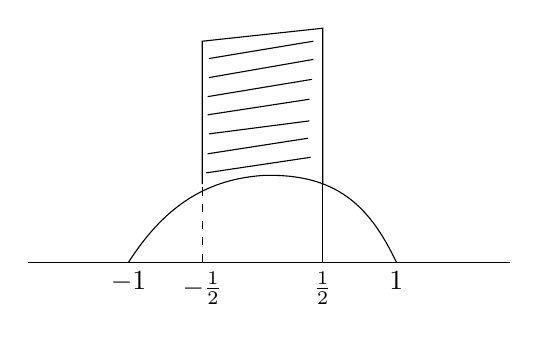
\begin{tikzpicture}[x=1.7cm,y=1.1cm]
\draw (-1.75,0) -- (1.85,0);
\draw (-1,0) .. controls (-0.75,0.6) and (-0.45,0.95) .. (0,1) .. controls (0.55,1.03) and (0.8,0.65) .. (1,0);
\draw[dashed] (-0.45,0) -- (-0.45,0.9);
\draw (0.45,0) -- (0.45,0.9);
\draw (-0.45,0.9) -- (-0.45,2.55) -- (0.45,2.7) -- (0.45,0.9);
\draw (-0.42,1.03) -- (0.36,1.21);
\draw (-0.41,1.25) -- (0.34,1.43);
\draw (-0.40,1.48) -- (0.35,1.63);
\draw (-0.41,1.70) -- (0.35,1.88);
\draw (-0.41,1.91) -- (0.37,2.11);
\draw (-0.40,2.13) -- (0.38,2.34);
\draw (-0.40,2.35) -- (0.38,2.55);
\node[below] at (-1,0) {$-1$};
\node[below] at (-0.45,0) {$-\frac{1}{2}$};
\node[below] at (0.45,0) {$\frac{1}{2}$};
\node[below] at (1,0) {$1$};
\end{tikzpicture}
\end{adjustbox}
[Справа от рисунка: это фунд. область.]

Плоскость — аналит. мн-зие всех эллипт. кривых.

\underline{\underline{Общее опр. 1}}

Есть совокупн. аналит. мн-зий $K$.

Пр-во модулей — аналит. мн-зие с отображением
\begin{adjustbox}{max width=\linewidth}
\begin{tikzcd}
X \arrow[d,"p"] \\
\underline{Y}
\end{tikzcd}
\end{adjustbox}

($X,\underline{Y}$ — мн. и анал. отобр.). Точки $\underline{Y}$ во вз. одн. соотв. с $K$
[После $K$ — три наклонных разделительных штриха.]
и, кроме того, $p^{-1}(y)\cong$ соотв. объекту из $K$

(объекты из $K$ не могут быть аналит. изом.)

\SourcePage{GELFAND-P000239}{2}
$\underline{Y}=K$ со структурой аналит. мн-зия

Если пр-во модулей сущ., то единств. с точн. до аналит. изом.
(легко док.).

Другое опред. учитывает возможные автоморфизмы объектов из $K$.

\underline{\underline{Предв. понятие.}}

[Слева в рамке: Анал.]
\underline{Сем-во объектов из $K$:}
\begin{adjustbox}{max width=\linewidth}
\begin{tikzcd}
X \arrow[d] \\
\underline{Y}
\end{tikzcd}
\end{adjustbox}
все слои изом. объектам из $K$

\underline{Индуцир. семейство} [подчёркивание прерывистое] — аналог. индуц. рассл.
(оно всегда существует)

\begin{adjustbox}{max width=\linewidth}
\begin{tikzcd}
X'' \arrow[r] \arrow[dr] \arrow[rr,bend left=25] & X' \arrow[r] \arrow[d] & X \arrow[d] \\
& Y' \arrow[r] & Y
\end{tikzcd}
\end{adjustbox}

Это коммут. диагр. $+$ универс.

\underline{Универсальность} [подчёркивание прерывистое; над концом слова дуговая стрелка влево.]

(
\begin{adjustbox}{max width=\linewidth}
\begin{tikzcd}
X' \arrow[d] \\
\underline{Y'}
\end{tikzcd}
\end{adjustbox}
универс.)

\begin{adjustbox}{max width=\linewidth}
\begin{tikzpicture}[x=1cm,y=1cm]
\draw (0,1.3) ellipse (0.17 and 0.4);
\draw (1.6,1.3) ellipse (0.16 and 0.4);
\draw (0,0) circle (0.04);
\draw (1.6,0) circle (0.04);
\end{tikzpicture}
\end{adjustbox}

просто коммут. диаграммы недостаточно
(2 точки и любой, где $\exists$ отображение).

\begin{adjustbox}{max width=\linewidth}
\begin{tikzcd}
Y'\times X \arrow[r] \arrow[d] & X \arrow[d] \\
Y' \arrow[r] & \bullet
\end{tikzcd}
\end{adjustbox}

[Подчёркнуто волнистой линией:] Кириллов (гипотеза)

Представимый функтор. Представляющий объект и есть сем-во модулей

2 катег. — 1) все аналит. пр-ва.

функтор в [зачёркнуто: \Unclear{GELFAND-P000239}{category-cancelled}{2)}] категорию множеств

$Y\rightsquigarrow$ мн-во пар
\begin{adjustbox}{max width=\linewidth}
\begin{tikzcd}
X \arrow[d] \\
\underline{Y}
\end{tikzcd}
\end{adjustbox}
— аналит. семейств.

Предст. функтора
\begin{equation*}
C\overset{F}{\longrightarrow}\mathrm{Ens}\quad (\text{мн-ва})
\end{equation*}
\begin{equation*}
F_M=\operatorname{Hom}(\bullet,M)\qquad M\text{ — аналит. пр-во.}
\end{equation*}

[Двойная горизонтальная черта.]

[Слева в рамке: Офиц. опр.]

\begin{adjustbox}{max width=\linewidth}
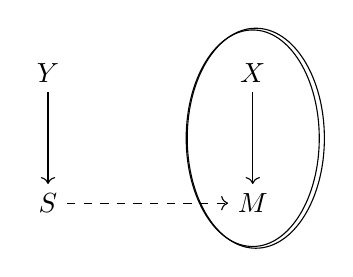
\begin{tikzpicture}[x=1.3cm,y=1.1cm]
\node (ys) at (0,1.5) {$Y$};
\node (ss) at (0,0) {$S$};
\node (xx) at (2,1.5) {$X$};
\node (mm) at (2,0) {$M$};
\draw[->] (ys) -- (ss);
\draw[->] (xx) -- (mm);
\draw[->,dashed] (ss) -- (mm);
\draw (2,0.75) ellipse (0.65 and 1.25);
\draw (2.03,0.75) ellipse (0.67 and 1.27);
\end{tikzpicture}
\end{adjustbox}
— сем-во наз. мн. модулей, если $\forall$ другое сем-во получ. как индуцир.
\SourcePage{GELFAND-P000240}{unlabelled}
Универс. сем-ва для кривых данного рода
не существует (даже для эллиптич.)

Сущ. для поляризованных (с выбр. базисом гомологий)

\underline{\underline{Видоизм.}} — финальный объект категории семейств

Если он не сущ., то присоед. формально.

Вводится доп. структ., позв. рассм. когом. с коэфф. в пучке
и т. д.

Не сущ. универс. объекта для элл. кривых

\SourceFigure{GELFAND-P000240}{oval-m}{Слева изображён вертикальный овал с прерывистой левой стороной; ниже и правее отдельно написано $M$. Связующая линия не видна.}

[Справа от рисунка:]
все точки однозн. отобр. $\Rightarrow$
как мн-во — элл. крив. не повтор.

Пусть есть нетрив. сем-во (база не точка) с
одинаковыми слоями.
[Над «слоями» вставлено: (расслоение).]
\Incomplete{GELFAND-P000240}{middle-cancel}{Небольшой зачёркнутый фрагмент справа от «слоями» не удалось прочесть.}

(т. к. есть автоморфизмы)

Тогда отобр. должно быть в точку и получ.
\Unclear{GELFAND-P000240}{lower-trivial}{трив. / нетрив.}

Существ. в более слабом смысле — плоскость

\SourceFigure{GELFAND-P000240}{margin-right-sketch}{На правом поле узкий четырёхсторонний контур с двумя утолщёнными вертикальными сторонами и несколькими поперечными штрихами. Справа сверху отдельный утолщённый знак, похожий на $M$; ниже — спутанные и зачёркнутые штрихи. Чтение этих знаков и их связь с контуром не установлены.}

У большинства один автом. ($x\to -x$) (с отм. точкой),
а у нек-рых ещё повороты.

\textbf{Итак}, работа сост. в том, что изучаются св-ва
несуществующего универс. объекта.

Начало точно $6^{\underline{15}}$

\SourcePage{GELFAND-P000241}{3}
$9/\underline{\overline{\mathrm{IX}}}$.
\underline{Продолжение} \underline{докл.} \underline{Геронимуса.}

Несуществование пр-ва модулей преодолевается фикс. базиса
гомол. (более жёсткий объект). Это не рассм.

Для эллипт. кривых фиксируется только точка (и то не
сразу).

\textbf{Будет указан путь (другой) преодол. этой трудности.}

Опред. топ. Гротендика.

Рассл. произв. над $S$ — пр. в катег.
$\begin{adjustbox}{max width=\linewidth}
\begin{tikzcd}[row sep=small]X\arrow[d]\\S\end{tikzcd}
\end{adjustbox}$.
[Под «над $S$» обведено: $X\times_S Y$.]

Акс. топ. Гротендика очев., кроме:
[зачёркнуто: $X_i\times Y$]
\begin{equation*}
\left.\begin{gathered}
X_i\longrightarrow X\text{ — покр.}\\
Y\longrightarrow X
\end{gathered}\right\}
\Rightarrow
\begin{gathered}
X_i\times_X Y\longrightarrow X\\
\text{покр.}
\end{gathered}
\end{equation*}
\Unclear{GELFAND-P000241}{base-change-target}{В правой части записано $X_i\times_X Y\to X$; конечная буква — $X$.}

Морфизм топологий Гротендика —

— функтор $T_1\to T_2$, сохр. все структуры.

\underline{Пример 1.} $T_\Gamma$ — $\Gamma$-множества ($\Gamma$ — группа).

Рассл. произв. сущ. — пары.

\begin{equation*}
\begin{adjustbox}{max width=\linewidth}
\begin{tikzcd}[column sep=small,row sep=small]
X\arrow[dr]&&Y\arrow[dl]\\
&Z&
\end{tikzcd}
\end{adjustbox}
\quad\text{даны.}\qquad
\begin{adjustbox}{max width=\linewidth}
\begin{tikzcd}[column sep=small,row sep=small]
&X\times Y\arrow[dl]\arrow[dr]&\\
X\arrow[dr,"p_1"']&&Y\arrow[dl,"p_2"]\\
&Z&
\end{tikzcd}
\end{adjustbox}
\end{equation*}
(в $X\times Y$ берутся пары $(x,y)$,
такие что $p_1(x)=p_2(y)$).

$X_i\overset{f}{\longrightarrow}X$ — покрытие, если
$\bigcup f_i(X_i)=X$.

Финальный объект
\Unclear{GELFAND-P000241}{terminal-cancel}{[плотные петлевидные штрихи перед тире; неразборчиво]}
— точка.

Когомологии точки с коэфф. в разл. пучках.
$H^q(\cdot,F)$

[Справа:] ($F$ — пучок, произв.)

[Зачёркнуто: На]
Все пучки устроены так.

Если задано знач. $F(\Gamma)=A$ ($\Gamma$ дейст. на $\Gamma$ слева),
то на всех ост. однозначно опр. группой $A$. (если
это в самом деле пучок, а не предпучок).

$\Gamma\longrightarrow\Gamma/H$ \qquad покрытие.

Св-во пучка применяем к покр. откр. мн-ва $\Gamma/H$. Получ.
\begin{equation*}
F(\Gamma/H)=A^H\qquad\text{(элем. $A$, инвар. отн. $H$)}
\end{equation*}
($\Gamma$ действ. на $A$, т. к. отобр. мн-в индуц. отобр. сечений
по опр. предпучка).

\SourcePage{GELFAND-P000242}{unlabelled}
Для произв. $\Gamma$-мн-ва, явл. объед. непересек. орбит, надо
рассм. вложения всех орбит и будет
\Unclear{GELFAND-P000242}{orbit-sum}{прямая сумма}.

\textbf{Итак}, все однозн. опр. $\Gamma$-модулем $A$.

При этом
\begin{equation*}
\underline{\underline{H^q(\cdot,F)=H^q(\Gamma,A)}}.
\end{equation*}
[Справа:] (иное опр. $H^q(\Gamma,A)$).

Факт о когом. групп
\begin{center}
\Unclear{GELFAND-P000242}{degree-two-characters}{$\displaystyle H^2(\Gamma,Z)=\{\text{все компл. одномерные представления }\Gamma\}$}
\end{center}

\underline{\underline{Пример 2.}} Топология $C$

Катег. аналит. мн-зий и их отобр. друг. в друга.
[Над «отобр.» обводками выделены вставки: открытые; аналит.
Нижний отросток обводки направлен к «отобр.».]
\Incomplete{GELFAND-P000242}{insertion-cancel}{Зачёркнутый фрагмент слева от «аналит.» внутри обводки не удалось прочесть.}

Есть рассл. произведение.

Покрытия (!) $X$ — аналит. мн-зие

$X_i\overset{f_i}{\longrightarrow}X$ — покр., если
\begin{enumerate}
\item[1)] $\bigcup f_i(X_i)=X$
\item[2)] каждое $f_i$ — неразветвлённое накрытие $X_i$
над откр. множеством $X$

($f_i^{-1}$ дискр. мн-во точек).
\end{enumerate}

\begin{equation*}
\begin{adjustbox}{max width=\linewidth}
\begin{tikzcd}[column sep=0.5em,row sep=0.4em]
X\arrow[dr]&\times&Y\arrow[dl]\\
&Z&
\end{tikzcd}
\end{adjustbox}
\quad\text{— совок. пар, проект. в одну точку $Z$}
\end{equation*}
(на нём ввод. аналит. структ.)

пусть $F$ дан на всей этой топологии
[Над $F$ обведена вставка: пучок.]
\begin{equation*}
H^q(X,F)=H^q(X,\widetilde F)
\end{equation*}
$\widetilde F$ — пучок на обычной топологии
(ограничение)

(обычные когомологии)

(над достат. малым откр. мн-вом все накрытия
распадаются).
\SourcePage{GELFAND-P000243}{4}
\underline{\underline{Пример 3.}} (основной) Дано $K$.

\begin{equation*}
\begin{adjustbox}{max width=\linewidth}
\begin{tikzcd}[row sep=small]
X \arrow[d] \\
S
\end{tikzcd}
\end{adjustbox}
\quad\text{— аналит. сем-ва объектов из $K$ (мн-зий)}
\end{equation*}
Отображение — индуцирование,
[зачёркнуто: \Unclear{GELFAND-P000243}{top-crossout}{все?}]
с открытым отобр. баз.
[Слова «с открытым отобр. баз.» выделены снизу угловой скобкой.]

Сущ. рассл. произведения
\begin{equation*}
\begin{adjustbox}{max width=\linewidth}
\begin{tikzcd}[row sep=small,column sep=small]
X_2 \arrow[rr] \arrow[d,"\pi"'] && X_1 \arrow[d,"\pi"] \\
S_2 \arrow[rr] \arrow[dr] && S_1 \arrow[dl] \\
& S &
\end{tikzcd}
\end{adjustbox}
\qquad\text{Надо взять}\qquad
\begin{adjustbox}{max width=\linewidth}
\begin{tikzcd}[row sep=small,column sep=small]
& S_2\times_S S_1 \arrow[dl] \arrow[dr] & \\
S_2 && S_1
\end{tikzcd}
\end{adjustbox}
\end{equation*}
и индуц. над ним сем-во (из $S_2$ и $S_1$ получ. одно и то же)

Покрытие
\begin{equation*}
\begin{adjustbox}{max width=\linewidth}
\begin{tikzcd}[row sep=small]
X_i \arrow[r] \arrow[d,"\pi_i"] & X \arrow[d] \\
S_i \arrow[r] & S
\end{tikzcd}
\end{adjustbox}
\end{equation*}
если образы покр. всё $S$ и каждое отобр. —
— накрытие (в смысле прим. 2).

\begin{equation*}
H^q(\pi,F)\quad\text{эквив. предыд. примеру}\quad
\cong\quad\text{когом. $S$ пред. примера.}
\end{equation*}
(т.к. структ. откр. множеств те же и топологии изоморфны).

[Под $H^q(\pi,F)$, перед следующей строкой:
\Unclear{GELFAND-P000243}{cohomology-vertical-sign}{вертикальный знак, напоминающий повёрнутое $\cong$}.]
\begin{equation*}
H^q(S,\widetilde F)\quad\text{— обычные когомологии.}
\end{equation*}
Если есть финальн. объект.

Пусть фин. \underline{объекта нет}.

\underline{\underline{Пример 4.}}

$T_M$ — катег. — старая $+$ форм. присоед. фин. объект $M$.
Считаются его когомологии, как если бы он сущ.

Сущ. расслоенное произведение.
\begin{equation*}
\pi\times_M M=\pi
\end{equation*}
[Справа:] ($M$ отобр. только в $M$)

Остаётся рассл. $X\times_M Y$

В любой категории $X\times_M Y$ — прямое произведение.
(тавтологич. факт).

(оно может быть и пустым
\Unclear{GELFAND-P000243}{bottom-final-sign}{знак, похожий на $\xi$, возможно зачёркнутый})

[Вписано снизу:] — есть пустое семейство

\SourcePage{GELFAND-P000244}{unlabelled}
Существование прямого произв. — трудная
[зачёркнуто: \Unclear{GELFAND-P000244}{top-cancelled-word}{категория?};
над строкой вставлено: теорема]
для категории семейств.

\begin{equation*}
\begin{adjustbox}{max width=\linewidth}
\begin{tikzcd}[row sep=small]
S_1\times S_2 \arrow[r] \arrow[d] & S_2 \\
S_1 &
\end{tikzcd}
\end{adjustbox}
\qquad\text{над $S_1\times S_2$ индуц. \underline{\underline{разные}} сем-ва}
\end{equation*}
и нельзя базу брать $S_1\times S_2$.

\begin{center}
\begin{adjustbox}{max width=\linewidth}
\begin{tikzpicture}[x=1cm,y=1cm]
\node at (0,1.9) {$X_1$};
\node at (2,1.9) {$X_2$};
\draw (0.22,1.4) circle (0.04);
\fill (2,1.35) circle (0.045);
\draw (0.2,0.65) circle (0.055);
\draw (1.8,0.65) circle (0.055);
\node at (0,0) {$S_1$};
\node at (2,0) {$S_2$};
\end{tikzpicture}
\end{adjustbox}
\end{center}
Если $X_1=X_2$ то произв. — оно само.
Если $X_1\ne X_2$, то пустое.

[Зачёркнуто: \Unclear{GELFAND-P000244}{left-cancelled-word}{Но?}]
Если точка, то как правило пустое.
Если близко к универс., то обычно непустое.

\begin{equation*}
\begin{adjustbox}{max width=\linewidth}
\begin{tikzcd}[row sep=small]
Y \arrow[d] & X \arrow[d] \\
\bullet & S
\end{tikzcd}
\end{adjustbox}
\end{equation*}
База — подмн-зие в $S$, со слоями, изом. $Y$.
если есть автом., то
[зачёркнуто: \Unclear{GELFAND-P000244}{multiplicity-crossout}{есть?}]
кратность и пр.

Теор. множ. — база — точки в $S$ со слоями $Y$,
кратность — число автоморфизмов.

Это — аналит. мн-зие! (трудная теорема)

(число способов \underline{отобр. $Y$ в} это сем-во)

\underline{Опред. покрытия} $M$:
\begin{equation*}
\pi_i\longrightarrow M\quad\text{— покр., если}\quad\pi\longrightarrow M
\end{equation*}
[Под строкой, с линией к $\pi\longrightarrow M$:] для любого другого
\begin{equation*}
\pi_i\times\pi\longrightarrow\pi\quad\text{— \underline{\underline{настоящее покрытие}}.}
\end{equation*}
(одна акс. этим опр. обеспечена, остальные — автоматич.)

Все $\pi_i$ — не покрытие!

[Зачёркнуто: \Unclear{GELFAND-P000244}{bottom-cancelled-word}{Но?}]
В след. раз продолжение и или резольвента Спенсера
\underline{\underline{или Dwork.}}

[В нижнем поле — жёлтый значок примечания с тремя горизонтальными штрихами.]

\SourcePage{GELFAND-P000245}{5}
$16/\overline{\underline{\mathrm{IX}}}$

Геронимус.
[Подчёркнуто волнистой линией.]

[Вверху справа, с линией к следующей фразе:]
(надо, чтобы сущ.
\Incomplete{GELFAND-P000245}{top-cancelled-word}{Зачёркнутое слово перед «рассл. произв.» не читается под несколькими густыми штрихами.}
рассл. произв.)

Извинения: всюду не аналит. мн-зия, а аналит. пр-ва.

Рассл. произведение.
\begin{equation*}
\forall\quad\left(
\begin{adjustbox}{max width=\linewidth}
\begin{tikzcd}[row sep=small,column sep=small]
X \arrow[dr] && Y \arrow[dl] \\
& Z &
\end{tikzcd}
\end{adjustbox}\right)
\qquad\exists\quad
\begin{adjustbox}{max width=\linewidth}
\begin{tikzcd}[row sep=small,column sep=small]
& X\times_Z Y \arrow[dl] \arrow[dr] & \\
X \arrow[dr] && Y \arrow[dl] \\
& Z &
\end{tikzcd}
\end{adjustbox}
\quad\text{(комм.)}
\end{equation*}
и универсально, т.е. если
\begin{equation*}
\begin{adjustbox}{max width=\linewidth}
\begin{tikzcd}[row sep=small,column sep=small]
& A \arrow[dl] \arrow[dr] & \\
X \arrow[dr] && Y \arrow[dl] \\
& Z &
\end{tikzcd}
\end{adjustbox}
\quad\text{, то}\quad
\begin{adjustbox}{max width=\linewidth}
\begin{tikzcd}[row sep=small,column sep=small]
& A \arrow[d] \arrow[ddl] \arrow[ddr] & \\
& X\times_Z Y \arrow[dl] \arrow[dr] & \\
X && Y
\end{tikzcd}
\end{adjustbox}
\end{equation*}

\underline{Аксиомы покрытия}

1) $X_{ij}\longrightarrow X_i\longrightarrow X$

2) $X\overset{e}{\longrightarrow}X$
\Unclear{GELFAND-P000245}{axiom2-arrow-label}{над стрелкой: $e$ или $\varepsilon$}

3) $X_i\times_X Y\longrightarrow Y$

Предпучок: контравар. функтор $F$ в кат. групп.
[Слово «Предпучок» подчёркнуто пунктиром.]

Пучок.
[Подчёркнуто пунктиром.]
\begin{equation*}
U_i\longrightarrow U\quad\text{— покрытие}
\end{equation*}
\begin{equation*}
g_i\in F(U_i)
\end{equation*}
\begin{equation*}
\begin{gathered}
U_i\longleftarrow U_i\times_U U_j\\
U_j\longleftarrow U_i\times_U U_j
\end{gathered}
\qquad
\begin{adjustbox}{max width=\linewidth}
\begin{tikzcd}[row sep=small,column sep=small]
g_i\in F(U_i) \arrow[r] & F(U_i\times_U U_j) \\
g_j\in F(U_j) \arrow[ur] &
\end{tikzcd}
\end{adjustbox}
\end{equation*}
Соглас., если $g_i$ перех. в один элемент.

\begin{equation*}
U_i\longrightarrow U\qquad F(U)\longrightarrow\underset{g_i}{F(U_i)}
\end{equation*}

[Зачёркнуто: \Unclear{GELFAND-P000245}{sheaf-cancelled-word}{опр.?}]
пучок: если \underline{\underline{сущ.}} и \underline{\underline{единств.}} $g\in F(U)$,
перех. в $g_i$.

\begin{equation*}
T^o\overset{F}{\longrightarrow}\mathrm{Ab}\qquad F\text{ — пучок.}
\end{equation*}
\Unclear{GELFAND-P000245}{bottom-category-symbol}{первый знак исправлен поверх написанного; $T^o$ или $T^0$}

[Под $T^o$, с пунктирной линией:] катег. с обр. стрелками.

[Под $\mathrm{Ab}$:] абел. группы
\SourcePage{GELFAND-P000246}{unlabelled}
% Источник: 1960 x 2392 пикселя. Координаты ниже отсчитываются от верхнего левого угла.
% Проверка «позв.»: bbox=(625,269,795,375), 3x/5x; сопоставлено с тем же сокращением P000240, bbox=(775,483,930,585), 5x. «по любом» сохранено буквально.
\underline{Когомологии} — это группы
\Unclear{GELFAND-P000246}{top-degree}{$H^q(U,F)$ или $H^{\nu}(U,F)$},
такие что $H^0(U,F)=F(U)$. и если
\begin{equation*}
0\longrightarrow F'\longrightarrow F\longrightarrow F''\longrightarrow 0,
\quad\text{то}
\end{equation*}
(есть процедура,
позв.
по любом предпучку канонически постр. пучок — для любой топологии),
\begin{equation*}
\longrightarrow H^q(U,F')\longrightarrow H^q(U,F)
\longrightarrow H^q(U,F'')\longrightarrow H^{q+1}(U,F')\longrightarrow\ldots
\end{equation*}
(они существуют).

И для любого инъект. пучка
\Unclear{GELFAND-P000246}{injective-degrees}{когом. $0$}
(и ин. пучк. дост. много)

Пусть есть отобр., совм. со всеми структ. (отобр. топологий)
\begin{equation*}
\begin{array}{ccc}
f:T_1&\longrightarrow&T_2\\
f^*F&\text{опр.}&F
\end{array}
\qquad
f^*F(U)=F(f(U)).
\end{equation*}
\begin{equation*}
H^q(U,f^*F)\longrightarrow H^q(f(U),F).
\end{equation*}

[В рамке:]

\Unclear{GELFAND-P000246}{boxed-degrees}{$U\longrightarrow H^i(f(U),F)$}
предп. и постр. пучок нулевой,
тогда это отобр. задает изом. канонический
(\Unclear{GELFAND-P000246}{criterion-word}{форм.} критерий)
\begin{equation*}
H^q(U,f^*F)\cong H^q(f(U),F).
\end{equation*}

[Конец рамки.]

\underline{Осн.} \underline{пример $T$.}
объекты — аналит. сем-ва
$\begin{adjustbox}{max width=\linewidth}
\begin{tikzcd}[row sep=small]X\arrow[d]\\S\end{tikzcd}
\end{adjustbox}$
($X,S$ — аналит. пр-ва)

[Зачёркнуто двумя горизонтальными линиями: Надо, что]
% Чтение отмены проверено по bbox=(100,1667,605,1771), 6x, и независимо (110,1680,430,1760), 7x; буквы «Надо, что» различимы между линиями.

\underline{Новая категория} $T_M$ с $M$. (фин. объектом)

Сущ. рассл. произведений.

[Подчёркнуто волнистой линией:]
Устройство покрытий финального объекта.
(топол. пр-ва модулей)

$\pi_i$ — покр.
\Unclear{GELFAND-P000246}{cover-crossout}{[зачёркнутый знак: $\varphi$ или о]}
$M$, если вып. св-ва

1) каждое $K$ сод. в виде слоя в одном из сем-в $\pi_i$

2) каждое $K$ сод. лишь дискр. число раз
\SourcePage{GELFAND-P000247}{6}
3) Аксиома продолжения. $\forall X$.

\underline{Каждое} $\Pi_i$ удовл. усл.
$\begin{adjustbox}{max width=\linewidth}
\begin{tikzcd}[row sep=small]
X \arrow[d,"\pi_i"'] \\
S
\end{tikzcd}
\end{adjustbox}$.

$\forall$ [вставлено над строкой и обведено: другого] \underline{сем-ва}
$\begin{adjustbox}{max width=\linewidth}
\begin{tikzcd}[row sep=small,column sep=small]
X' \arrow[d] & X \arrow[d] \\
S' & S
\end{tikzcd}
\end{adjustbox}$
[вертикаль $X\to S$ обведена овалом]
и подсем-ва (база — подмногообр.
и [зачёркнуто: \Unclear{GELFAND-P000247}{cancelled-abbreviation}{т.д. / т.е.}] индуц. огран.)
и $\forall$ отобр. подсем-ва
$\exists$ его продолжение (локальное)-
\newline
— в трубчатую окрестность $S''$.

\SourceFigure{GELFAND-P000247}{extension-diagram}{Слева под текстом схема с $X'$ вверху слева, $X$ вверху справа и $X''$ между ними ниже. От $X'$ к $X$ видна пунктирная стрелка вправо; от $X''$ к $X$ — диагональная стрелка вверх вправо. От $X'$ вниз идёт стрелка к $S'$, от $X''$ вниз — к $S''$. Справа внизу стоит $S$; от $S''$ к $S$ идёт диагональная стрелка вверх вправо. Между $S'$ и $S''$ виден знак, похожий на $\supset$. Горизонтальный участок от $S'$ к $S$ многократно перечёркнут; его окончательное состояние требует проверки по оригиналу.}

В следующий раз — \underline{пример с эллипт. кривыми.}

[Внизу слева — заштрихованный прямоугольный знак:]
\begin{adjustbox}{max width=\linewidth}

\begin{tikzpicture}[x=0.35cm,y=0.35cm]
\draw (0,0) -- (0,1.1) -- (0.7,1.2) -- (0.7,0.1);
\draw (-0.12,0.2) -- (0.73,0.78);
\draw (-0.12,0.45) -- (0.73,1.01);
\draw (-0.12,0.7) -- (0.68,1.2);
\draw (0,0.05) -- (0.77,0.54);
\draw (0.35,-0.1) -- (0.76,0.23);
\end{tikzpicture}
\end{adjustbox}

\SourcePage{GELFAND-P000248}{unlabelled}
\underline{\underline{Паламодов.}}

\underline{Резольвента Спенсера.}

Работают
\newline
Sweeny
\newline
\Unclear{GELFAND-P000248}{names-second}{Holdschmidt / Heldschmidt / Goldschmidt}
\newline
Guillemin
\newline
Quillen
\newline
Sternberg
\newline
Singer

[Справа, за вертикальной чертой:] изложено Sweeny в Acta math.

Способ решать систему $p(x,D)u=w$, где $p$ — матрица,
$u,w$ — векторы.

$M$ — гладкое многообразие. $\mathcal O$ — пучок ростков дифф. ф-й.

\begin{equation*}
\begin{adjustbox}{max width=\linewidth}
\begin{tikzcd}[column sep=large]
\mathcal O \arrow[r,"j_\mu"] & J_\mu
\end{tikzcd}
\end{adjustbox}
\end{equation*}
[Под $J_\mu$, с дуговой чертой: джеты пор. $\mu$ (струи).]
($j_\mu$ даже вложение)

$J_\mu$ — вект. расслоение (или пучок его ростков)
\begin{equation*}
\begin{adjustbox}{max width=\linewidth}
\begin{tikzcd}[column sep=large]
\mathcal O \arrow[r,tail,"j_\mu"] & J_\mu.
\end{tikzcd}
\end{adjustbox}
\end{equation*}
[Слева в этой стрелке знак исправлен:
\Unclear{GELFAND-P000248}{second-sheaf}{повторно обведённое $\mathcal O$ / $\mathcal O$ с приписанным верхним знаком}.]

Резольвента Спенсера пучка $\mathcal O$ начинается с $j_\mu$
и продолж., чтобы посл. пучков была точна.
\begin{equation*}
0 \longrightarrow \mathcal O \overset{j_\mu}{\longrightarrow} J_\mu \longrightarrow
\end{equation*}
$\mu=0$ — отобр. в $0$.

Дан набор (проект И.М.Г.)
\begin{equation*}
\varphi_i \qquad i\text{ — мультииндекс},\qquad |i|\leq\mu.
\end{equation*}
\begin{equation*}
f\overset{j_1}{\longrightarrow}
\begin{gathered}
\varphi_0(x)=f(x)\\
\varphi_1(x)=\dfrac{\partial f}{\partial x_1}\\
\varphi_2(x)\\
\vdots
\end{gathered}
\qquad
\varphi_i=\frac{\partial\varphi_0}{\partial x_i}
\qquad
\frac{\partial\varphi_0}{\partial x_i}-\varphi_i
\end{equation*}
в пр-во, изом. $J$-м 1-го порядка

[Горизонтальная черта.]

Сравн. с \Unclear{GELFAND-P000248}{bottom-comparison}{псевдогр. / псевдооп.} на порядок выше.
\begin{equation*}
f\longrightarrow\{D^i f\}.
\end{equation*}

\SourcePage{GELFAND-P000249}{7}
обозначение $1_j=(0,\ldots,\underset{j}{1},\ldots,0)$

ср. $\varphi_i$ с $\varphi_{i+1_j}$.

Надо \Unclear{GELFAND-P000249}{top-abbreviation}{прв. / пров.}, что
\begin{equation*}
\frac{\partial\varphi_i}{\partial x_j}=\varphi_{i+1_j},
\qquad
\underset{|i|\leq\mu-1}{\forall i},\qquad j=1,\ldots,n.
\end{equation*}

Отобр. в [зачёркнуто: \Unclear{GELFAND-P000249}{upper-cancellation}{$J$ / $j$}; начало следующего слова также исправлено]
джеты на $1$ меньшего порядка.
\begin{equation*}
\{\varphi_i\}\longrightarrow
\left\{\frac{\partial}{\partial x_j}\varphi_i-\varphi_{i+1_j}\right\}
\end{equation*}
\begin{equation*}
|i|\leq\mu-1,\qquad j=1,2,\ldots,n.
\end{equation*}
\begin{equation*}
\sum\left(\frac{\partial}{\partial x_j}\varphi_i-\varphi_{i+1_j}\right)dx_j
\qquad\text{(добавили).}
\end{equation*}
\begin{equation*}
\begin{adjustbox}{max width=\linewidth}
\begin{tikzcd}[column sep=large]
(\mathcal O) \arrow[r,tail] & J_\mu \arrow[r,"D"] & T^*\otimes_{\mathcal O}J_{\mu-1} \arrow[r,"D=d-\delta"] & \Lambda^2 T^*\otimes_{\mathcal O}J_{\mu-2}
\end{tikzcd}
\end{adjustbox}
\end{equation*}
[Под $T^*$, с дуговой чертой: кокас.]

\begin{equation*}
\left(\frac{\partial}{\partial x_j}\varphi_i-\varphi_{i+1_j}\right)
=(d-\delta)\{\varphi_i\}
\end{equation*}
(разность опер. фактич. и формального дифф.)

На $T^*\otimes J_{\mu-1}$ тоже опр. оба опр.

$d$ — внешн. дифф. по 1-й коорд.

$\delta$ — формальное дифф.

\begin{equation*}
\{\varphi_i^j(x)dx_j\}
\overset{D=d-\delta}{\longrightarrow}
d(\varphi_i^j(x)dx_j)-\varphi_{i+1_s}^j\,dx_j\wedge dx_s
\end{equation*}
[В последнем коэффициенте нижний индекс исправлен:
\Unclear{GELFAND-P000249}{lower-corrected-index}{$i+1_s$ / $i+1_j$}.]

и т.д.

Резольвента оборвется (и она точна)

[Справа — жёлтый значок комментария без видимого текста.]

След.-раз Геронимус, Паламодов и Каждан

\SourcePage{GELFAND-P000250}{unlabelled}
23/IX

\underline{Геронимус.}

$K$ — пр-во всех торов с компл. структурой, и с отмеч. точкой.
Построим топ. Гротендика. Категория: семейства
\begin{center}
\begin{adjustbox}{max width=\linewidth}
\begin{tikzcd}
X \arrow[d,"\pi"'] \\
S
\end{tikzcd}
\end{adjustbox}
\end{center}
с выделенным сечением $\sigma\colon S\to X$
(аналит. отобр.)

\SourceFigure{GELFAND-P000250}{lattice-domain}{Слева нарисованы горизонтальная ось со стрелкой вправо и вертикальная ось со стрелкой вверх; на горизонтальной оси подписаны $-1$, $-\frac12$, $\frac12$, $1$. Над осью проходит дуга, похожая на полуокружность; на ней три жирные точки. От двух боковых точек вверх идут почти вертикальные линии, между которыми верхняя область заштрихована наклонными штрихами; от этих точек вниз к оси идут короткие линии. Справа от заштрихованной области проведён короткий горизонтальный штрих к следующей подписи. Точная форма границ и соединения штрихов неуверенны.}

мн-во всех решёток $S'$

(пр-во модулей в грубом смысле слова)

[Под словом «грубом»:] (coarse)

Топ. Гротенд. — пр-во мод. в тонком (fine) см. слова.

Фактор $H/\Gamma$ — $H$ — верхн. полуплоскость

Есть сем-во с базой $S'$, но это не тонкое пр-во
модулей

(не индуцир. нетрив. рассл. с пост. слоем)

Другая причина.
\begin{center}
\begin{adjustbox}{max width=\linewidth}
\begin{tikzcd}
H \arrow[d] \\
H/\Gamma
\end{tikzcd}
\end{adjustbox}
\end{center}
Сем-во над $H$ не индуцир. с сем-ва над $H/\Gamma$.

(При действ. на $H$ есть неподв. точки (3 штуки)
там ветвление
\SourceFigure{GELFAND-P000250}{branching-sketch}{Между словами «ветвление» и «и получ.» помещён маленький рисунок: от густо обведённого округлого узла отходят пять штрихов — вверх, влево, вправо, вниз влево и вниз вправо. На концах и в месте соединения есть утолщения; нельзя уверенно отличить наконечники от повторного обведения.}
и получ. разные структ. элл. кривой)

Сем-во над $H$ \qquad $H\times\mathbb{C}$ \qquad $z\in H$ \qquad $(z,1)$ —
— решётка.

[Обведено:]
\begin{equation*}
\fbox{$(z,\zeta)\sim(z,\zeta+mz+n)\qquad \operatorname{Im}z>0.$}
\end{equation*}
\begin{equation*}
z'=\frac{az+b}{cz+d}.
\end{equation*}

\underline{Задача: это семейство,}

\SourcePage{GELFAND-P000251}{8}
\underline{и там действует группа}
\begin{align*}
z'&=\frac{az+b}{cz+d}\\
\zeta'&=\zeta(cz+d)^{-1}
\end{align*}

[На верхнем правом поле зачёркнуто: \Unclear{GELFAND-P000251}{top-right-cancellation}{там / так}.]

\underline{\underline{Подсчёт когомологий в этом случае.}}

\underline{Топология и всё прочее определялось ранее.}

[Зачёркнуто отдельное слово: \Unclear{GELFAND-P000251}{cancelled-leading-word}{Когом. (?) / неразборчивое слово}.]

[Зачёркнуто: $H^n(\pi,Z)=$ это пучок]

\begin{equation*}
F(\pi)=\underbrace{Z+Z+Z}_{\text{по числу связн. комп.}}
\end{equation*}
(так сказать, пост. пучок).

Легко видеть, что $H^n(\pi,Z)=H^n(S,Z)$

[Под левой частью:] ($\pi$ — обычн.) \qquad [Под правой частью:] (Топологич.).

Когом. фин. объекта.

1) $T_\Gamma$ — другой топ.; $\Gamma$ — группа матриц с $\det 1$.

2) $T'_\Gamma$ — те $\Gamma$-мн-ва, где $\Gamma$ не слишком трив. действ

(если стац. подгр. $\forall$ точки — целоч. матр. с
[зачёркнуто: \Unclear{GELFAND-P000251}{stabilizer-cancellation}{неразборчивое слово}]
$1\ \mathrm{mod}\ 3$.
\begin{equation*}
\sigma x=x\to\sigma\in\Gamma_3.)
\end{equation*}

Отображение $T'_\Gamma\to T$
\begin{equation*}
S\to(H\times S)/\Gamma\qquad (S\text{ — дискр. мн-во}).
\end{equation*}
\begin{equation*}
M'\to M.
\end{equation*}
Оно индуц. изоморфизм когомологий.

(что проверяется из указанного в прошлый раз критерия).

Отсюда
\begin{equation*}
H^n(M,Z)=H^n(\Gamma,Z)=
\begin{cases}
0 & n\ne 2\\
Z_{12} & n=2
\end{cases}
\end{equation*}
\Unclear{GELFAND-P000251}{cohomology-degree}{Условия в правой части прочитаны как $n\ne2$ и $n=2$; сильно обведённый знак во втором условии допускает также чтение $n\equiv2$. Область значений $n$ здесь не уточнена.}

(но если бы $\Gamma$ действ. без неподв. точек совп. с
когом. обычн. пр-ва модулей).

Ответ верен над любым полем ($\operatorname{Char}\ne2$).

[На нижнем правом поле, после двух вертикальных черт:]
У сем-в есть инвар. $\mathrm{mod}\ 12$.

\SourcePage{GELFAND-P000252}{unlabelled}
\underline{Шафаревич:} пример топ. Гротендика

Дана сист. дифф. ур-ий (обыкн.) на \Unclear{GELFAND-P000252}{manifold-abbreviation}{мн-зии / мн-гии}

$U$ — трансверс. площадка

Отобр.
\SourceFigure{GELFAND-P000252}{trajectory-sketch}{Слева написано $U$, затем нарисован высокий овал, а правее — меньший овал. Две длинные кривые пересекаются между овалами; одна из них образует большую петлю справа от меньшего овала. Внутри левого овала два коротких жирных штриха около пересечений, похожих на стрелки влево; внутри правого овала также видны короткие окончания линий. Уверенно установить направления всех стрелок и точные соединения линий невозможно.}

[Справа от рисунка:]
$U\to V$

если из точек $U$
пров. [зачёркнуто: \Unclear{GELFAND-P000252}{trajectory-cancellation}{по (?) / неразборчивое слово}] траект. в $V$

есть рассл. произведение
\SourceFigure{GELFAND-P000252}{fiber-product-sketch}{Маленький рисунок справа: три округлых контура — вверху слева, внизу посередине и вверху справа. От нижнего к каждому верхнему идут по две близкие наклонные линии, образуя V-образную фигуру. В контурах есть короткие штрихи, местами похожие на стрелки или буквы; точные подписи, соединения и направления не читаются уверенно.}

Если расслоение, то когом. базы и сист. трив.

(тогда есть фин. объект).

\underline{\underline{На плоск.}} дифф. ур-е и пост. пучок топ. Грот.,
то его Эйлерова хар. — разность [вставлено над строкой и обведено: чисел]
\Unclear{GELFAND-P000252}{cycles-abbreviation}{прд. / пред.} циклов
и особ. точек.

В след. раз \underline{\underline{Каждан.}} и \underline{\underline{Паламодов.}}

\SourcePage{GELFAND-P000253}{9}

$30/\underline{\overline{\mathrm{IX}}}$. \underline{Каждан.}

\underline{Раб. Ихара.} (яп.). (Ihara, Journ. Math. Soc. of J.\Incomplete{GELFAND-P000253}{bibliography-erasure}{Далее два мелких вертикальных штриха: возможно, 11 или II; продолжение библиографической записи под плотным зачёркиванием не читается.}
\underline{107-121})

Одномерные пов. на $C$ связ. с дискр. группами.

Попытка переноса на кривые над конечными полями.

$X=\Gamma\backslash M$ \qquad $M$ — пл. Лобач.

$\Gamma$ опис. не только $X$, но и неразветвл. накрытия.

(The \Unclear{GELFAND-P000253}{english-title}{congruence / conguence} monodromy problem).

В [\Unclear{GELFAND-P000253}{cancelled-ring-symbol}{Зачёркнутый знак перед кольцом: возможно, $C$ или $k$.}]
$k[X,Y]$ рассм. главный идеал $(f)$

$A=k[x,y]/(f)$ — кольцо ф-й на кривой, макс. идеалы — геом. точки кривой

Отобр. $Y\longrightarrow X$ это отобр. колец $A\longrightarrow B$

$B\longleftarrow A$

Неразветвл. отобр. — неразв. в $\forall$ точке.

$\underset{\text{макс. идеал.}}{m}\subset A$ \qquad Рассм. образ. и \underline{\underline{$B/mB$}}

если не сод. нильпот. элем., то неразветвлено в $m$.

\underline{В след. понедельник семинара не будет.}

Через раз будет...

\SourcePage{GELFAND-P000254}{unlabelled}

$14/\underline{\overline{\mathrm{X}}}$ \underline{Паламодов.}

$X$ — мн-зие

$O$ — пучок ростков дифф. ф-й.

\begin{adjustbox}{max width=\linewidth}
\begin{tikzcd}[column sep=large]
O \arrow[r, tail] & J^k
\end{tikzcd}
\end{adjustbox}
— пучок джетов пор. $k$.

предпучок
$\{\varphi_i,\quad i=(i_1,\ldots,i_n),\quad |i|\le k\}$
\qquad переход — как у производных.

\underline{Гельфанд.} Опрд.

Пусть $k,m$ — целые числа.

Опрд. $(m,k)$-джетов.
\Unclear{GELFAND-P000254}{jet-tuple}{Первая буква пары переписана поверх прежних штрихов: $(m,k)$ / $(n,k)$.}

$X$ — дифф. мн-зие.

Рассм. ф-и от $(m+1)$-го переменного.
\Unclear{GELFAND-P000254}{variable-count}{Буква перед $+1$ также обведена: $m+1$ / $n+1$.}

(обычные — $(1,k)$-жеты).

\underline{$(1,k)$-жеты.}

$\varphi(x,y)$ — ф-и на квадрате $X\times X$

Рассм. диагональ $x=y$

Рассм. совок. ф-й $=0$ на диагонали

Это идеал.

% Правое добавление отделено от основного текста двумя вертикальными чертами.
\begin{flushright}
$m\ne1$ \qquad $\overbrace{X\times\cdots\times X}^{(m+1)\ \text{раз.}}$

диаг. $x_1=x_2=\cdots=x_{m+1}$

$\mathcal J$ — идеал.
\Unclear{GELFAND-P000254}{ideal-symbol}{Рукописное обозначение идеала: $\mathcal J$ / $\mathcal I$; далее сохранён тот же знак.}

$\varphi(x_1,\ldots,x_{m+1})=0$ если

$x_1=x_2=\cdots=x_{m+1}$
\end{flushright}

Рассм. \underline{\underline{$\mathcal J^{k+1}$}} \qquad (ф-и $k$-го пор. малости на диаг.)

Считаем $\varphi_1\sim\varphi_2$, если $\varphi_1-\varphi_2\in\mathcal J^{k+1}$

\SourceFigure{GELFAND-P000254}{diagonal-square}{Небольшой квадрат с толстой диагональю из левого нижнего в правый верхний угол; оба нижних угла утолщены. В середине диагонали виден дополнительный тёмный знак, неуверенно различимый как точка или наконечник. Подписей нет.}

$\varphi(x,y)$ — [\Unclear{GELFAND-P000254}{cancelled-single-symbol}{Маленький зачёркнутый знак: возможно, $0$ или $e$.}]

$(1,0)$-джет. — ф-я на диагонали.

\Incomplete{GELFAND-P000254}{cancelled-jet-expression}{Слева от следующей строки зачёркнута короткая запись. Возможное начало — $(1,$; остальное перекрыто штриховкой и не читается.}
$(1,1)$ — джет \Unclear{GELFAND-P000254}{jet-zero-or-sheaf}{$0$ / $O$} на диаг. с $1$-ми произв.

\begin{gather*}
\varphi(x,y)=\varphi(x,x)+\left.\frac{\partial\varphi(x,y)}{\partial x}\right|_{y=x}(y-x)
\\
\varphi(x,y)=\varphi(y,y)+\left.\frac{\partial\varphi(x,y)}{\partial y}\right|_{y=x}(x-y)
\end{gather*}
\Unclear{GELFAND-P000254}{derivative-variables}{В первой формуле виден знаменатель $\partial x$, во второй — $\partial y$; эти переменные сохранены буквально.}

Есть $2$ способа опр. джеты

\begin{gather*}
a(x)+b(x)(y-x)
\\
a(y)+b(y)(x-y)
\end{gather*}
это различные способы.

\SourcePage{GELFAND-P000255}{10}

Можно дифференцировать — будет джет меньшего порядка.

\begin{equation*}
\varphi(x_1,\ldots,x_{n+1})=\varphi(x,\ldots,x)+\sum\left.\frac{\partial\varphi}{\partial x_i}\right|_{\ldots}
\end{equation*}
\Unclear{GELFAND-P000255}{unfinished-taylor-end}{После вертикальной черты видны маленькие точки или штрихи на уровне нижнего индекса; формула здесь обрывается.}

$(1,m)$-джет — скал. ф-я $+$ дифф. форма

\underline{\underline{Паламодов.}}

Случай общего $m$ свод. к $m=1$.

\begin{equation*}
\varphi(x,y)\sim\sum_{|i|\le m}\varphi_i(x)\frac{\xi^i}{i!}
\end{equation*}

\begin{equation*}
O_Y\longrightarrow O_{X\times Y}/\mathcal J^{k+1}
\end{equation*}
\Unclear{GELFAND-P000255}{quotient-ideal-symbol}{В знаменателе рукописный знак идеала: $\mathcal J^{k+1}$ / $\mathcal I^{k+1}$.}

\begin{adjustbox}{max width=\linewidth}
\begin{tikzcd}[column sep=small]
0 \arrow[r] & O_X \arrow[r,"j"] & J^k \arrow[r,"d_x"] & T^*\otimes J^{k-1} \arrow[r,"d_x"] & \Lambda^2 T^*\otimes J^{k-2} \arrow[r] & \ldots
\end{tikzcd}
\end{adjustbox}

Резольв. Спенсера (трив. случай)

\underline{\underline{В общ. случае}} — $O_X$ зам. на пучок ростков реш. произв. лин. сист. ур-й.

Sweeny

\underline{Acta Math., $120\ N=3-4$.}

и \underline{разработка Malgrang'a}

Quillen — большая статья в трудах...

\underline{След. раз:} Паламодов опять.

\SourcePage{GELFAND-P000256}{17}
% Original PNG: 1984 x 2416. Review coordinates below use the original pixel grid.
$27/\overline{\underline{\mathrm{X}}}$. Проф. \underline{\underline{Вайнштейн}} (USA).

\underline{об операторах.}

4/\Unclear{GELFAND-P000256}{schedule-date}{XI / X}
\underline{\underline{Кириллов}} — \underline{Следы операторов} !!

$11/\overline{\underline{\mathrm{XI}}}$ — \underline{\underline{пропускали.}}

$18/\overline{\underline{\mathrm{XI}}}$ \underline{\underline{Каждан}}
$\zeta$-ф-и по Дворку

$25/\overline{\underline{\mathrm{XI}}}$ —\,''\,——\,''\,——\,''\,——
[Три знака повтора на длинной горизонтальной черте под предыдущей строкой.]

\underline{\underline{Кириллов.}}

$\mathcal A$ — оператор.

$M$ — комп. мн-зие, \qquad $\mathcal L_2(M,H)$ \qquad $H$ — гильбертово.

$\mu$ — мера на нём

(или эрмитово расслоение)

\begin{equation*}
\mathcal K f(x)=\int_M K(x,y)f(y)\,d\mu(y)
\end{equation*}

($K$ — операт. ф-я, \quad $K(x,y)\colon H\longrightarrow H$)

непр. по совок. арг. в слабой опер. топологии.

[Слева, над следующей строкой:] Сущ. следа

Необх., а для [вставлено над строкой в обводке: опер.] $>0$ достат. сущ.

\begin{equation*}
\operatorname{tr}\mathcal K=\int_M\operatorname{tr}K(x,x)\,d\mu(x)
\qquad (\operatorname{tr}\text{ в обычн. смысле}).
\end{equation*}
[Формула выделена снизу чертой с загнутыми вверх концами.]

Скалярн. ф-и см. Гохберг и Крейн (теор. Карлемана)

\underline{\underline{Нетрив.:}} если $\mathcal K$ имеет след, то
$\operatorname{tr}K(x,x)$ сущ. почти всюду.

\underline{Вайнштейн.}

$A$ — самосопр. опер. с дискр. спектром.

\begin{equation*}
\mathbf{A+B}\qquad \min R(u)\qquad R(u)=\frac{(Au,u)}{(u,u)}
\end{equation*}

Ур-е Эйлера даёт
\Unclear{GELFAND-P000256}{euler-sign}{$Au=\lambda u=0$}

[Справа под дробью:]
\Unclear{GELFAND-P000256}{lower-right-space}{$u\perp\mathcal R$}

[Под обозначением пространства:] беск.-мерн.

\begin{equation*}
\mathcal P=\bigcup\mathcal P_n
\end{equation*}
\begin{equation*}
\min_{u\perp\mathcal P_n}R(u)
\qquad \text{сущ. реш.:}\quad \det\ldots=0
\end{equation*}
\SourcePage{GELFAND-P000257}{unlabelled}
\begin{equation*}
\min_{u\perp\Unclear{GELFAND-P000257}{top-min-condition}{\Phi\ \text{или}\ P}}
\frac{(Au,u)}{(u,u)}
\end{equation*}
сущ. для опр. \underline{Шредингера}

(не только вполне непр.).

\underline{Вообще.} классич. теория --- оценки соб. знач., с одной стор.

Вайнштейн и К$^{\circ}$ --- с другой стороны.

\underline{Ко-то из Польши.}\quad \underline{Ролевич.}

\underline{Периодич. решения дифф. ур-й с запаздыванием.}

Свод. к реш. сист. обыкн. ур-й с период. коэфф.

[Справа, у скобки, охватывающей две строки:]
периодич. \Unclear{GELFAND-P000257}{right-delay-margin}{случ.?}

Ещё немн. приложений и пр.

Прим. к задачам управления.

Будет \underline{Кириллов.}

\medskip
4/XI\qquad \underline{Кириллов.}

$G$ --- односв. группа Ли

$T$ --- неприв. представление

\begin{equation*}
T(\varphi)=\int_G\varphi(g)T(g)\,dg\quad\text{--- оператор}
\end{equation*}

[Справа:] $\operatorname{tr}$ как обобщ. ф-я иногда сущ.

\begin{equation*}
\operatorname{tr}T(\varphi)=\int_G\varphi(g)\chi(g)\,dg
\end{equation*}

$\chi(g)$ --- обобщённая ф-я

В примерах она не сложнее, чем мера, но общей
Теоремы нет.

Есть прим., когда нет следа ни при каких $\varphi$ и
даже более узк., чем $C_0^{\infty}$.

\begin{equation*}
\begin{pmatrix}a&b\\0&1\end{pmatrix}
\end{equation*}
для неё надо сузить $C_0^{\infty}$ до ф-й с
\begin{equation*}
\int\varphi(a,b)\,db\underset{a}{\equiv}0
\end{equation*}
(по классу сопр. элем. --- $0$)

\SourcePage{GELFAND-P000258}{18}
$\mathfrak{g}$ --- алг. Ли,\quad
$\mathfrak{g}^{*}$ --- двойств. пр-во

[Под обоими обозначениями:] (вещ.)\qquad (вещ.).

$G$ действ. в $\mathfrak{g}$ и $\mathfrak{g}^{*}$.

$\chi(g)$ похожа на другую обобщ. ф-ю.

$\mathfrak{g}^{*}\supset\Omega$,\qquad $\Omega$ --- орбита $G$.

$\Omega$ --- симплект. пр-во (там есть невырожд. 2-форма).

\begin{center}
\begin{adjustbox}{max width=\linewidth}
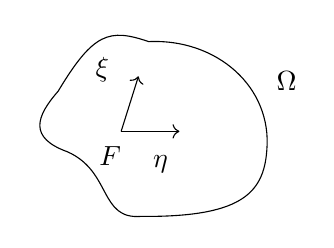
\begin{tikzpicture}[x=1cm,y=1cm]
\draw (0.1,1.45) .. controls (0.55,2.2) and (0.75,2.25) .. (1.25,2.08)
.. controls (2.12,2.12) and (2.82,1.5) .. (2.75,0.7)
.. controls (2.71,0.13) and (2.39,-0.15) .. (1.15,-0.14)
.. controls (0.62,-0.18) and (0.78,0.43) .. (0.22,0.68)
.. controls (-0.28,0.86) and (-0.18,1.13) .. (0.1,1.45);
\draw[->] (0.9,0.94) -- (1.12,1.64);
\draw[->] (0.9,0.94) -- (1.64,0.94);
\node at (0.66,1.72) {$\xi$};
\node at (1.4,0.52) {$\eta$};
\node at (0.76,0.63) {$F$};
\node at (3,1.58) {$\Omega$};
\end{tikzpicture}
\end{adjustbox}
\end{center}

$B(\xi,\eta)$

$F\in\Omega$

ф-л на $\mathfrak{g}$.

\begin{equation*}
\begin{adjustbox}{max width=\linewidth}
\begin{tikzcd}
0\arrow[r]&\mathcal{H}\arrow[r]&\mathfrak{g}\arrow[r]&T\Omega_F\arrow[r]&0
\end{tikzcd}
\end{adjustbox}
\end{equation*}

[Под $\mathcal{H}$:] стац. подалг. орбиты $\Omega$.

[К $T\Omega_F$ проведены линии от помет:]
кас. пр-во к орбите [обведено];
(из транзит. --- перенос).

\begin{equation*}
\begin{adjustbox}{max width=\linewidth}
\begin{tikzcd}
\xi&\eta\\
X\arrow[u]&Y\arrow[u]
\end{tikzcd}
\end{adjustbox}
\end{equation*}

Надо взять
\begin{equation*}
\frac{1}{2\pi}\langle F,[X,Y]\rangle=B(\xi,\eta)
\end{equation*}
[Справа, подчёркнуто:]
\underline{кососимм.}\quad
\underline{невырожд.}\quad
\underline{форма}.

(корректно --- не зав. от выбора
[зачёркнуты два обозначения:
$\Unclear{GELFAND-P000258}{middle-cancelled-symbols}{\text{неразборчиво; }\xi,\eta\ \text{или}\ X,Y}$]
предст. $\bmod\mathcal{H}$)

\underline{Неоднор. форма.}
\begin{equation*}
\beta=e^B=1+B+\frac{B\wedge B}{2!}+\cdots+
\frac{B\wedge\cdots\wedge B}{k!}
\end{equation*}
(он обрывается).

На самом деле для интегр. нужен один член.

Итак, опр. мера на каждой орбите.

\begin{equation*}
\text{обобщ. ф-и}\quad
\left\{
\begin{aligned}
\mathcal{J}_{\Omega}(x)&=\int_{\Omega}e^{i\langle F,X\rangle}\beta(F)\\[8pt]
\chi(\exp X)&
\end{aligned}
\right.
\end{equation*}
[К первой строке:] (преобр. Фурье меры на орбите).

\noindent\rule{12cm}{0.4pt}

похожи друг на друга.

гипотеза о совпадении \underline{неверна}.\qquad Но:

\SourcePage{GELFAND-P000259}{unlabelled}
Их отношение $\in C^{\infty}$ и можно написать формулу.

$\forall$ неприв. предст.

\begin{equation*}
\chi(\exp X)=p_{\Omega}^{-1}(x)\int_{\Omega}e^{i\langle F,X\rangle}\beta(F),
\end{equation*}

где
\begin{equation*}
p_{\Omega}(x)=
\begin{cases}
1&\text{для нильпот. групп}\\
\sqrt{\Unclear{GELFAND-P000259}{upper-density-symbol}{\rho\ \text{или}\ g}(x)}
&\text{для орбит общего полож. (для всех групп)}\\[6pt]
\sqrt[4]{\Unclear{GELFAND-P000259}{upper-density-product}{\rho_{\ell}(x)\rho_n(x)\ \text{или}\ g_{\ell}(x)g_n(x)}}
&\text{[зачёркнуто: для] (если нет инв. меры).}
\end{cases}
\end{equation*}

[Под выражением во второй строке, с дугой от него:]
инв. мера (если она есть).

[Пометы слева к $p_{\Omega}$:]
$p_{\Omega}(0)=1$

\underline{гладкая} (доказано)

(орбиты не всегда соотв. представлениям)

\SourceFigure{GELFAND-P000259}{middle-curved-arrow}{Толстая изогнутая стрелка справа от пометы «Нильп. гр.» поднимается через строку о компактной группе; верхний наконечник находится около слов «не всегда», под формулой с корнем четвёртой степени. Точное отнесение стрелки неясно.}

\underline{Для произв. комп. группы все орб. общего положения.}

\underline{Нильп. гр.}

\underline{Редукц. \Unclear{GELFAND-P000259}{middle-reduction-heading}{теоремы}}

\begin{equation*}
\Unclear{GELFAND-P000259}{middle-modified-sh-definition}{\operatorname{sth}\ \text{или}\ \overline{\operatorname{sh}}}\,x
=\frac{\operatorname{sh}\frac{x}{2}}{x/2}
\end{equation*}

\begin{equation*}
p_{\Omega}(x)=\prod_{\alpha}
\Unclear{GELFAND-P000259}{middle-modified-sh-product}{\operatorname{sth}\ \text{или}\ \overline{\operatorname{sh}}}
\langle\alpha,X\rangle
\qquad\text{(гипотеза)}
\end{equation*}

(где $\alpha$ --- корни)

\medskip
\underline{Унит. неприв. предст. всех групп Ли.}

в $\mathfrak{g}^{*}$ орбиты $\Omega$.

Выбрать те; для к-рых $B\in H^2(\Omega,\mathbb{Z})$

($\int$ по $\forall$ циклу --- целый)

\underline{Целочисл. орбите} ответ. предст.
[зачёркнуто:
\Incomplete{GELFAND-P000259}{lower-cancelled-quantity}{Короткий зачёркнутый фрагмент не прочитан полностью.}]
[Вставлено сверху, в обводке: в кол-ве]
равному \underline{числу характеров фунд. группы орбиты}.

(фунд. гр. коммутативна в этом случае).

\SourcePage{GELFAND-P000260}{19}

[Зачёркнуто: На.] Для $SU(2)$ (почти $SO(3)$)

2 форма на сфере $\frac{1}{2\pi}\frac{d\sigma}{r}$.

Целочисленность: \fbox{$2r=n$} — такие сферы.

$\int\ldots=\frac{\sin rx}{x}$. Получ. обычные характеры.

\Unclear{GELFAND-P000260}{top-radius-symbol}{В трёх формулах знак, условно переданный как $r$, читается как $r$ либо $\tau$.}

\underline{Универс. ф-ла Планшереля для всех групп.}

\begin{equation*}
\int_G |f(g)|^2\,dg=\int\operatorname{tr}[T(f)T^*(f)]\,d\mu(T)
\end{equation*}
\begin{equation*}
T(f)=\int_G f(g)T(g)\,dg
\end{equation*}

($T$ пробег. все непр. унит. предст. с точн. до эквив.)

Абстр. теор. — верна, вопрос в вычисл. меры $d\mu$.

\underline{\underline{Задача.}} Для кососимм. матрицы из её $\det$ извлеч. полиномиальный кв. корень.

(пример $\det\begin{pmatrix}0&a\\-a&0\end{pmatrix}=-a^2$).
[Перед матрицей мелко, ниже строки, вставлено $\det$; верхний левый нуль обведён повторно.]
\Unclear{GELFAND-P000260}{middle-determinant-sign}{В источнике перед $a^2$ отчётливо написан минус: $-a^2$.}

[Две короткие горизонтальные черты.]

\underline{Одна нетрив. двойств.:}

[Левый столбец.]

1) Произвед. матриц, к-рые $>0$.
[Над $>0$ вставлено: (унит.).]

Найти распред. соб. знач.
по распр. соб. знач. сомнож.

[Двойная вертикальная черта отделяет правый столбец.]

2) то же для тенз.
произв. предст. унит. группы.

Переломов и Попов —

— о выпукл. области.

[Ниже обоих столбцов.]

$[(x^2-1)^n]^{(n)}$ — Лежандр

$[(x-1)^{m_1}(x+1)^{m_2}]^{(m_3)}$ — полиномы Якоби

$m_3$ — дробн. — гипергеом. ф-я

(или $x(x-1)$)
[Начало слова «или» обведено повторно. Внизу справа жёлтый значок примечания с тремя горизонтальными штрихами; видимого текста внутри нет.]

\SourcePage{GELFAND-P000261}{unlabelled}

18/XI.
[Над и под XI проведены черты.]

\Incomplete{GELFAND-P000261}{top-cancelled-heading}{Рядом с датой густо зачёркнутый, дважды подчёркнутый заголовок; текст под зачёркиванием не читается.}

\underline{Лит-ра по теории представлений.}

\underline{\underline{Минимум}} (\underline{0-й уровень})

1. Лекции Кириллова „Элем. теор. предст.“, I, II

2. Гельфанд, Минлос, Шапиро „Предст. группы вращений“

3. Желобенко, Лекции по теор. предст.

4. Джекоб Шварц „Алг. Ли и группы Ли“ (англ)

5. Серр — „ —
[После фамилии знак повтора: короткая черта, две кавычки, длинная черта.]

6. Винберг „Компактные группы Ли“.

7. Семинар Софус Ли „Предст. алгебр Ли и предст. групп Ли“
[«и» вставлено ниже строки между «Ли» и «предст.».]

1. общие теор. о кон. и комп. гр.

2. подр. разбор для гр. вращ. и матр. 2-го пор. — иллюстр. и конкр. к 1.

3. полезно для физиков

4. общая теория групп Ли и класс. комп. и полупр. Групп

6. ... комп. группы и алгебры Ли (Шварц, но короче)

7. совр. излож. теории полупр. групп

[Некоторые номера в обоих списках обведены повторно. Горизонтальная черта.]

\underline{1-й уровень.}

1. \underline{Гельфанд, Наймарк} [Зачёркнуто: Предст.] „Унит. предст. класс. групп“

(Акад. наук 1950)

(не читать главу про теор. Планшереля,

читать введ. и ст. \underline{Гельфанда и Граева} в Трудах мат. общ. т. 4.

(теор. Планшереля).

2. \underline{Годеман} Матем. 5:5

Простое док-во теор. Хариш-Чандра о сущ. хар.

Там же опис. кон-мерн. предст.

3. \underline{Березин} Труды т. 6 + письмо в ред. т. 12
[«т. 6» написано под «Труды», «т. 12» — под «письмо в ред.».]

[Зачёркнуто: \Unclear{GELFAND-P000261}{lower-berezin-cancelled-word}{Дан / Для}.] Опис. предст. полупр. группы через опер. Лапласа

Доказано сущ. всех предст.

4. \underline{Кириллов} Предст. нильпот. групп.

\SourceFigure{GELFAND-P000261}{lower-left-insertion-arrow}{Слева от строки «Макки» обведённый кружком, многократно исправленный номер, похожий на 7 или 4. От кружка идёт дуга влево и вверх, со стрелкой вверх у левого поля; точное отнесение стрелки к тексту неясно.}

\underline{Макки} Добавл. к кн. Сигала (\Unclear{GELFAND-P000261}{lower-mackey-abbreviation}{индуц. / индук.} предст.)

[Под кружком:] (в 0-й)

5. $SL(2,C)$, [Зачёркнуто: \Unclear{GELFAND-P000261}{bottom-cancelled-group}{обозначение, похожее на $SL_2$ или $SL(2)$}.]

(5-й вып. обобщ. ф-й, Наймарк, Унитарные пр. гр. Лоренца)

\SourcePage{GELFAND-P000262}{20}

$SL(2,R)$ (5-й вып. обобщ. ф-й)

[Горизонтальная черта.]

$SL(2,Q_p)$ (6-й вып. об. ф-й) [Зачёркнуто: или ст. Гельфанда )]

в след. уровень.

1-й уровень: нет оконч. теорем, кроме раб. Березина + Хариш-Чандра

6. Дж. Шварц, $C^*$-алгебры$^*$; Наймарк, УМН

[Под «$C^*$-алгебры»:] (книга)

[Горизонтальная черта.]

\underline{2-й уровень.}

1. $SL(2,Q_p)$. Об. ф-и 6.

2. Карпелевич, Гиндикин (Изв. АН) [Зачёркнуто: Метод.] Теор. Планшер.

для симм. пр-в.

3. Метод орисфер $\to$ 1-й уровень

(Гельфанд, Граев — Труды ММО, т. 8

4. Изложение [Зачёркнуто: Хариш-Чандры; над зачёркнутым вставлено: Серра.]
[Зачёркнуто: \Unclear{GELFAND-P000262}{middle-serre-cancelled-symbol}{о / одиночный неразборчивый знак}.] раб. Бореля-Вейля! в

— сем. Бурбаки (exp 100 или 101)

5. Излож. Хариш-Чандры на сем. Бурбаки (Брюа, [Зачёркнуто: \Unclear{GELFAND-P000262}{middle-bruhat-cancelled-symbol}{а / одиночный неразборчивый знак}.] Картье, Диксмье) —

— перев. в журн. „Математика“, 6:5

6. Группы и алг. типа 1, Глимм, Ферр и т. д. —

— в кн. Диксмье „$C^*$-алгебры и их предст.“

\Unclear{GELFAND-P000262}{lower-overwritten-heading-number}{Перед заголовком густо исправленный номер: 7 / 8.}
\underline{Алгебры Ли и обёрт. алгебры.}

7. \underline{Оберт. алгебры:}

а) Софус Ли; гл. I.

[Справа от пункта а):] б) Хариш-Чандра из 5)

в) Гельф., Кириллов; фр. работа и журн. ФА, т. 3 вып. 1

[Под «фр. работа»:] (Publ. Math.)

[Перед пунктом г) зачёркнуто: \Unclear{GELFAND-P000262}{bottom-cancelled-list-label}{в) / 8. / неразборчивый номер}.]
г) Костант, Amer. Journ., 85, стр. 327–404

д) Желобенко „Оберт. алг.“

е) Нельсон „Анал. вектора“ (есть перев. в журн. Матем.)

[Под названием журнала справа:] 6:3

\SourcePage{GELFAND-P000263}{unlabelled}
8. Кириллов и \Unclear{GELFAND-P000263}{top-kostant}{Костант / Костент}

\Unclear{GELFAND-P000263}{top-cancelled-sign}{[Слева от следующей строки — неразборчивый штриховой знак.]}
Общ. теория предст. и характеров.
\newline
(докл. на сем. Гельфанда

9. Хариш-Чандра — раб. последней серии. (с. 1963 г.)

10. Каждан — функц. анализ и франц. перевод на сем. Бурбаки.
\newline
т. I, вып. 1.
\newline
[Справа, под строкой о переводе:] (докл. Кириллова)

11. $G/\Gamma$ — обширная лит-ра (конференция Boulder)
\newline
[Под словом «Boulder»:] \Unclear{GELFAND-P000263}{boulder-note}{Sommer Scool / Sommer Sicol}
\newline
Proceed. — перевод готовится.

12. Другие поля. Обширная лит-ра,

\Unclear{GELFAND-P000263}{list-corrected-number}{13 / 14 [номер исправлен]}. Другие вопросы. — // —

[Горизонтальная разделительная черта со стрелкой вправо.]

13. Список вопросов.
\newline
Всё будет в „Успехах“

[Двойная горизонтальная разделительная черта.]

\underline{\underline{Громов.}}

1. \underline{Инвар. опр. дифф. опер.}

$M$ — мн-ие
\newline
$\mathcal L$ — рассл.
\newline
[От «рассл.» стрелка вверх и вправо к помете:] слой не обяз. лин. пр-во
\newline
$\Gamma(\mathcal L)$ — сечения.
\newline
[Справа:] $X$ — пр-во рассл.

Струя — класс эквив. сеч. с совп. с точн. до производных.

$\mathcal L^r$ — струйное расширение.
\newline
[Справа:] $X^r$ — его пр-во

Дифф. ур-е в частн. произв. —
\newline
— подмн-во $A\subset X^r$.

В прилож. — подмн-ие (не обяз. замкнутое),
\newline
лин. ур-е — подрасслоение.
\newline
(добавл. к $X$ вект. пр-ва)

\begin{equation*}
\mathcal L^r=\{M,X^r,\mathcal F^r,\Unclear{GELFAND-P000263}{bundle-projection}{\rho^r\text{ / }p^r}\}
\end{equation*}

Подмн-ие $A$ в класс. теор. обычно замкнуто.
\newline
Но ур-я $Lu\ne0$ — откр. мн-во
\newline
$L(u)=0$ — замкн. (если ф-я не удовл., то

\SourcePage{GELFAND-P000264}{21}
Или \underline{\underline{пример.}}

\begin{equation*}
f:\underset{g_1}{M_1}\longrightarrow\underset{g_2}{M_2}
\qquad\text{с кв. формами.}
\end{equation*}
гладк. отобр., индуц. формы \quad $f^*(g_2)=g_1$.

\begin{adjustbox}{max width=\linewidth}
\begin{tikzcd}
 & X=M_1\times M_2 \arrow[dl] \\
 M_1 &
\end{tikzcd}
\end{adjustbox}
[Справа:] отобр. $M_1\to M_2\Leftrightarrow$ сечение
\newline
доб. откр. усл. — чтобы было \underline{\underline{вложение.}}

\underline{Общая постановка:}
\newline
сущ. решение или нет.

\begin{equation*}
d^r:\Gamma(\mathcal L)\longrightarrow\Gamma(\mathcal L^r)
\qquad\text{(сеч. имеет джет в точке).}
\end{equation*}

\underline{\underline{Решение}}:
\Unclear{GELFAND-P000264}{solution-symbol}{$\gamma\in\Gamma(\mathcal L)$, если $\mathrm{Im}\,\gamma\subset A$ / $\delta\in\Gamma(\mathcal L)$, если $\mathrm{Im}\,\delta\subset A$}
\newline
[Под правой частью:] (в любой точке)

1. \underline{Проблема} \underline{существования.}
\newline
\underline{Связь} с \underline{другими}

[Номер «2.» перечёркнут косой чертой.]
\newline
2. \underline{Единств.} никогда не бывает (почти никогда)
\newline
[Под словами «почти никогда»:] откр. мн-ва
\newline
Но можно гов. о корректности.

3. \underline{Корректность.}
\newline
Сем-во $A_N$ дифф. ур-й
\quad (\Unclear{GELFAND-P000264}{family-subscript}{$A_N$ / $A_n$ / $A_\alpha$} варьируется)

\begin{equation*}
\Gamma(\mathcal L)\times N\longrightarrow N
\end{equation*}

Корректн. — это есть рассл. Серра!!!
\newline
[Под словом «Корректн.»:] \underline{\underline{сем-ва задач.}}

[Справа:]
\newline
(для [Зачёркнуто: всякого \Incomplete{GELFAND-P000264}{serre-cancelled-tail}{Далее зачёркнутый фрагмент: различимы знаки, похожие на $N$ и «и»; остальное неразборчиво.}]
\newline
всякого $\Gamma$ [Зачёркнутый знак: \Unclear{GELFAND-P000264}{serre-cancelled-sign}{неразборчиво}], сем-во $N$ фиксир.)

[В рамке:]
\newline
(можно напр. деформ.
\newline
с конечн. числом пар.)

\underline{Пример:}
\begin{equation*}
\underset{g_1}{M_1},\ \underset{g_2}{M_2}
\qquad\text{пара форм опр. ур-е}
\end{equation*}
Все пары форм — $N$,

\underline{Идея:} как правило, предполаг., что локально всё известно,
\newline
а что глоб. — неизв.
\newline
\underline{Лок. часть:} теоремы о неявных ф-ях Нэша.
\newline
[Мелко под словами «Лок. часть»:]
в прим.

\SourcePage{GELFAND-P000265}{unlabelled}
Уст. Корр. позв. решать ур-я
\newline
\underline{Теорема $C^1$-Нэша.}
\newline
задача $C^1$-погр. пост. корректна:
\newline
за деформ. метрики можно деформ. погружение.
\newline
С какой-то метрикой погр. сущ. — топ. ср-ва,
\newline
потом деформ. её в любую — получ. влож. !!

\underline{\underline{Принцип Уитни-Смейла \Unclear{GELFAND-P000265}{heading-continuation}{продолж. / продолже.} деформации.}}

Реш. над $U\subset M$,

\SourceFigure{GELFAND-P000265}{deformation-diagram}{Небольшой овальный контур; слева внутри него — изогнутая почти вертикальная линия, ограничивающая узкую часть с зигзагообразными штрихами. Точное соединение внутренней линии с нижней границей овала неясно; буквенных подписей уверенно не различить.}

[Справа от рисунка:]
\newline
над частью деформ. решение
\newline
распр. на всю обл.

(если игнор. краев. эффект)
\newline
Они док. его в ряде случаев.

[Зачёркнуто одной чертой: Из корр. и этого принц. можно]

Микроскопич. выполнимость этих принципов —
\newline
— это теор. о неявной ф-и.
\newline
(продолж. лишь в 1-й момент).

\underline{Часто бывает:}
\begin{equation*}
\text{Микро}\Rightarrow\text{Макро}
\end{equation*}
[Справа от «Макро» — изогнутая стрелка вниз.]

\underline{Сужение класса ур-й.}
\newline
Если [Затёртый знак: \Unclear{GELFAND-P000265}{before-solution-sign}{неразборчиво}] реш. после действ. диффеом. нек-рой группы ост.
\newline
решением, то \underline{\underline{Стабильность.}}
\newline
(инвар. отн. действ.
\newline
группы \underline{\underline{всех}} дифф., к-рая там действует в $X$ —
\newline
— если это задано)

пример — \underline{\underline{кас. рассл.}}
\newline
(ур-е переводит в себя)

[Слева зачёркнуто и подчёркнуто: Зад. Плато]

\underline{Пример:} зад. Плато
\begin{equation*}
R^2\longrightarrow R^3
\end{equation*}
[Справа:] миним. пленки инвар. отн.
\newline
диффеом.

Тогда (в стаб. случае) микро $\Rightarrow$ макро.

\underline{\underline{Другой принцип.}}
\quad [Над началом условий:] (Теорема 2.)

a) $M$ \Unclear{GELFAND-P000265}{parallel-abbreviation}{паралл. / парал.}
\newline
некомп. связн.

b) $A$ — подмн-ие
\newline
(подрасслоение)
\newline
и слои непуст.

[Под заголовком «Другой принцип», слева от условий:]
$\Rightarrow$

[Внизу страницы:]
13-04 с 16-18 вторн.; сем. \underline{Арнольда}

\SourcePage{GELFAND-P000266}{22}

c) есть \underline{Микро}

d) есть \underline{стабильность}

Тогда \underline{\underline{ур-е имеет решение}}.

Она содержит теорию погружений Смейла и т. д.

\underline{Некомп.}: микро $\Rightarrow$ макро.

[На правом поле, в рамке:]
\begin{equation*}
\fbox{$\begin{gathered}
\text{некомп.}\Rightarrow\\
\Rightarrow\text{есть ф-я без}\ \max
\end{gathered}$}
\end{equation*}

\underline{Пример геом. характера}
[Подчёркнуто волнистой линией.]

\underline{$M^n$ — риманово}
[Подчёркнуто волнистой линией.]

\begin{equation*}
M^n\subset R^s\qquad\text{лок. в}\quad
\underbrace{s=\frac{n(n+1)}{2}}_{\text{комп. метр. тензора}}
\end{equation*}

нельзя, вообще говоря, влез. в более низкое.

[Зачёркнуто: Но, \Incomplete{GELFAND-P000266}{middle-cancelled-line}{остаток зачёркнутой строки не поддаётся уверенному чтению}.]

Но: если $f_1,f_2:M\to$
\Unclear{GELFAND-P000266}{middle-target-exponent}{$R^{s}$ с замаранным знаком перед $s$; возможно, $R^{2s}$ или $R^{\lambda s}$}.

[Справа:]
\begin{equation*}
\underline{0<\lambda<1}
\end{equation*}
[Ниже справа зачёркнуто:]
\Incomplete{GELFAND-P000266}{middle-right-cancelled-formula}{неразборчивая зачёркнутая формула; различимы отдельные петли и нижний знак, похожий на $g_0$}.

[Между строками под отображением, слово «гладкое» обведено:]
гладкое параметриз. (стабильность).

они $C^0$-аппроксим. отобр. $\varphi_1,\varphi_2$, что
индуц. метрики одинаковы.
[Под предложением проведены две черты; нижняя заканчивается слева стрелкой.]

(Существенно нет однозн. определенности)

В больших разм. $t\ge s$

[Справа, дважды подчёркнуто:]
\Unclear{GELFAND-P000266}{lower-dimension}{$t=s+An$ или $t=3+An$}.

\begin{equation*}
M\to R
\end{equation*}
\Unclear{GELFAND-P000266}{lower-target-dimension}{[В отображении $M\to R$ показатель у $R$ не виден.]}

любое отобр. аппрокс. подобным
[под словом «подобным» зачёркнуто:
\Incomplete{GELFAND-P000266}{lower-cancelled-word}{замаранное слово; возможно, «изометрическим», но чтение не установлено}]
\Unclear{GELFAND-P000266}{lower-overwritten-symbol}{$f$ или $t$; знак переписан}
(с индуц. метрикой $\lambda g$)

Всё это следует из теоремы 2.

\underline{След. раз}: Громов
\SourcePage{GELFAND-P000267}{unlabelled}
% Original scan 1984 x 2416; coordinates in the ledger are original pixels,
% with origin at upper left and rectangles [x0,y0,x1,y1).
\subsection*{25/XI}
[Справа от даты зачёркнуто: \Unclear{GELFAND-P000267}{cancelled-date}{неразборчивый знак}.]

\underline{Олейник}\qquad рез. Радкевича по ур-ям
\begin{equation*}
Pu\equiv a^{ij}u_{x_i x_j}+b^i u_{x_i}+cu=0.
\end{equation*}
\Unclear{GELFAND-P000267}{drift-index}{В члене $b^i u_{x_i}$ последний индекс исправлен: $i$ или $j$.}

гипоэлл. --- ?

Хёрмандер:
\begin{equation*}
\sum_{i=1}^{n}X_i^2u+X_0u+cu=f
\end{equation*}
если в $\forall$ точке есть $n$ лин. незав. коммутаторов, то гипоэлл., что
получ. из оц.:
\begin{equation*}
\lVert u\rVert_{\varepsilon}\le C\bigl[\lVert u\rVert_0+\lVert Pu\rVert_0\bigr]
\end{equation*}
[В конце оценки зачёркнуто: \Unclear{GELFAND-P000267}{cancelled-norm}{$+{}$ слаб. норм}.]
\fbox{$\varepsilon>0$}\qquad (необх. не доказана)

\underline{Общий случай}: не прибегая к конкр. виду

[Слева в рамке, соединено линией с оценкой: «для оценки усл. необходимо».]

\underline{Радкевич}:
\begin{equation*}
Lu=a^{ij}u_{x_i x_j}+\gamma u
\end{equation*}
\begin{equation*}
P^0=a^{ij}u_{ij},\qquad P^{(j)}=a^{ij}(x)D_i,\qquad
P_{(j)}\underset{\text{сглаж. эллипт.}}{\underbrace{\mathcal E_{-1}}}
\end{equation*}
Операторы эти и все коммутаторы.
[Над словом «эти» проведена стрелка вправо.]

Условие то же самое

($2n$ опер. 1-го пор.)
\begin{equation*}
P_{(j)}=\sum_{i,k}\frac{\partial a_{ik}}{\partial x_j}
\frac{\partial^2}{\partial x_i\partial x_k}\bigl(\mathcal E_{(-1)}\bigr)
\end{equation*}
Ранг $n$ --- можно выделить эллиптическую систему.

1-й порядок --- то же самое

\underline{без псевдодифф. опер.}
\begin{equation*}
P^{(j)}\quad\text{и}\quad P_{(j)}
\end{equation*}
всюду оставляем главн. части

Надо, чтобы можно было получить эллипт. систему.

Формулировки, включ. теор. Хёрмандера пока нет.

\SourcePage{GELFAND-P000268}{25}
\underline{Гельфанд}: для приложений важно знать: когда любое решение
--- суммируемая функция?

\subsection*{Каждан}
Раб. \underline{Дворка}: рац. $\zeta$-ф-и $\forall$ алг. мн-зий над кон. полем.

$k$ --- поле.
\Unclear{GELFAND-P000268}{ideal-letter}{$A=k[x_1,\ldots,x_n]/\mathfrak J$}
--- афф. схема

Точки --- замкн. точки ($\max$ идеалы)

Теор. Гильберта:
\begin{equation*}
K=A/I\quad\text{--- конечн. расшир. }k.
\end{equation*}
Прост. идеалы --- точки.\qquad $K\supset k$.

Геом. точка со знач. в $K$: гомоморфизм $A\to K$.

(ему соотв. $\max$ идеал)
\begin{equation*}
A=\frac{R[x]}{x^2+1}
\end{equation*}
2 геом. точки, хотя 1 схемная

$i$ и $-i$

\underline{Алгебр. мн-зие} --- если нет нильпот. элементов

(это отличие от схемы)

[Слева зачёркнуто: \Unclear{GELFAND-P000268}{cancelled-before-field}{неразборчивый знак}.]
$F_{p^n}$ --- кон. поле, расш. $Z_p$ по ур-ю

\Unclear{GELFAND-P000268}{finite-polynomial}{$f(x)=\dfrac{x^{p^{n-1}}-1}{x^p-1}=0$.}

[В левом поле:]
\begin{equation*}
\begin{adjustbox}{max width=\linewidth}
\begin{tikzcd}
K\\
k\arrow[u]
\end{tikzcd}
\end{adjustbox}
\end{equation*}
Группа автом. $K$ циклична и имеет
канонич. обр. --- автом. Фробениуса
\begin{equation*}
\underline{\sigma:\ x\to x^p}.
\end{equation*}
\underline{$k=Z_p$.}

[Над следующей строкой: \Unclear{GELFAND-P000268}{interlinear-mark}{3. или §.}]

$A$ --- алгебр. мн-зие.\qquad $\zeta$-ф-я его --- ?

Рассм. замкн. точку $A$ --- $x=I\subset A$

$A/I$ --- конечное поле --- расшир. нек-рой степени.

Степень --- степень замкнутой точки.

\SourcePage{GELFAND-P000269}{unlabelled}
\begin{equation*}
\zeta(t,A)=\prod_{x\in X}\frac{1}{1-t^{\operatorname{deg}x}}
\end{equation*}
($t$ --- формальное переменное)

\underline{Теорема}. (Дворк)

$\forall$ алг. [Вписано над строкой: «аффинного».] мн-зия --- это рац. ф-я $t$

(была гипотеза Вейля, для кривых доказана ранее).

\underline{Точек обычно бесконечное число.}

Если $A$ --- кольцо [Вписано: «всех».] многочл. над $Z_p$, то
[Под строкой, в рамке: $Z_p[x]$.]
\begin{equation*}
\zeta(t)=\frac{1}{1-pt}
\end{equation*}
(разлож. беск. и все --- \Unclear{GELFAND-P000269}{poles-at-one}{полюса в 1})

\underline{Степень 1} --- ровно $p$ штук точек ($x$ --- $Z_p$).

\underline{Степень 2} --- в $(p^2-p)$ элем.

(чтобы не попад. в учтённые

$\exists\,1$ нетрив. автом.
\begin{equation*}
\frac{1}{(1-t)^p}\quad
\frac{1}{(1-t^2)^{\frac{p^2-p}{2}}}\quad
\frac{1}{(1-t^3)^{\frac{p^3-p}{3}}}\quad\ldots
\end{equation*}
[Ниже, отдельно:]
\Unclear{GELFAND-P000269}{fourth-factor}{$(1-t^4)^{\frac{p^4-p^2}{4}}$; цифры 4 исправлены, после $p^2$ зачёркнут знак.}

Единственность --- ?

\underline{Идея}

Степень подб. по посл. шансу уравн. коэфф. при посл.

Отсюда $\forall$ можно разложить.

\SourcePage{GELFAND-P000270}{26}
\begin{equation*}
\zeta(t,A)=\sum c_kt^k\qquad c_k\text{ --- целые}\qquad (\text{очев.}).
\end{equation*}
Имеет место равенство.
\begin{equation*}
\zeta(t,A)=\exp\left(\sum N_e t^e/e\right),
\end{equation*}
где $N_e$ --- число геом. точек со знач. в поле с $\operatorname{deg}=e$.

(число гомом. $A$ в $F_{p^e}$).

Это общее рав-во.

Но [Зачёркнуто: \Unclear{GELFAND-P000270}{cancelled-word}{сразу?}.]
из него сразу не след., что $c_k$ --- целые

Посчит. для $Z_p[x]$.\qquad $N_e=p^e$.
\begin{equation*}
\sum (pt)^e/e=-\ln(1-pt)\qquad\text{и далее ясно.}
\end{equation*}
Применим при $A=Z$. Будет обычная $\zeta$-ф-я.

[Зачёркнутая строка: \Incomplete{GELFAND-P000270}{cancelled-line}{Возможно, «Идея … Дворк»; текст под штриховкой не прочитан полностью.}]

\underline{Идея док-ва}. Ряд $\zeta(t,A)$ от компл. перем. --- сх. в круге.

Рассм. его от $p$-адич. перем. Тоже будет сход.
для малой нормы.

Мером. $p$-адич. (отнош. голом. $p$-адич.) $\Longrightarrow$

$\Longrightarrow$ автом. рацион. (общая теорема) ---

--- простая теорема
\begin{align*}
\mathbb Z_p\text{ --- кольцо}&=\{x\in Q_p;\ |x|\le1\}\\
M_p&=\{x\in Q_p:\ |x|<1\}\quad\text{--- макс. идеал}
\end{align*}
\begin{equation*}
\mathbb Z_p/M_p=Z_p\quad\text{--- поле из }p\text{ элем.}
\end{equation*}
\begin{equation*}
x_n\in Q_p.\qquad
\underset{\text{сход.}}{\sum x_n}\ \Longleftrightarrow\ x_n\to0.
\end{equation*}
Банаховы пр-во --- переносится обычн. опр.

Вполне непр. опер.

\SourcePage{GELFAND-P000271}{unlabelled}
\underline{Теор.} В бан. пр-ве вп. непр. опер. \underline{ядерный},
[Зачёркнуто: \Unclear{GELFAND-P000271}{cancelled-top}{то? или по…?}.]
и потому сущ. $\underline{\det(1-tA)}$

--- целая $p$-адич. ф-я от $p$-адич. перем. $t$.

\underline{Алгебр. расширения $Q_p$.}

[Зачёркнуто: «Замыкание».]

$\Omega$ --- алг. пополн. алг. замыкания $Q_p$
\begin{equation*}
Z_\Omega/\underset{\text{max идеал}}{\underbrace{M_\Omega}}=F\quad\text{--- поле}
\end{equation*}
Сущ. представителей Тейхмюллера.

У любого элем. $f\in F$ сущ. кан. представитель в $Z_\Omega$.
\begin{equation*}
\underline{F^*\longrightarrow Z_\Omega^*}\qquad\text{есть кан. гомоморфизм.}
\end{equation*}
\underline{Устройство аналит. ф-й на поле $p$-адич. чисел.}
\begin{equation*}
f(t)=\sum c_kt^k,\qquad c_k\in\Omega.
\end{equation*}
Целая аналит., т.е. $c_k$ дост. быстро $\to0$.

Тогда в $\forall$ [Зачёркнуто: \Unclear{GELFAND-P000271}{circle-insertion}{неразборчивое слово}; над строкой вписано и обведено: «круге».]
конечного радиуса конечн. число нулей.

\Unclear{GELFAND-P000271}{noncompact-unit-ball}{(Ед. круг в поле $Q_p$ не компактен)}

(Шнирельман)

\underline{Док-во}: принцип $\max$, лемма Шварца $\Rightarrow$ конечн. число нулей.

[Обведено над дробью: «рац. ф-я».]
\begin{equation*}
f(z)=\frac{\prod(1-\alpha_i z)}{\prod(1-\beta_j z)}=1+\sum c_kz^k
\end{equation*}
$c_k$ --- целые

$\alpha_i,\beta_j$ --- алгебр. $\Longrightarrow$ они целые алгебраич.

Если не целые, то получ. противоречие с нормами
\begin{equation*}
|\ |<1\quad\text{(в лев. части)}\qquad\text{справа }=1
\end{equation*}
(Это пример)

[Внизу мелко: «след. засед. в 1-й понед. след. сем.)»;
над «понед.» вписано: \Unclear{GELFAND-P000271}{next-session}{строго после 6/II}.]

[Внизу справа жёлтый значок комментария, без раскрытого текста.]

\SourcePage{GELFAND-P000272}{unlabelled}
\subsection*{10/II-1969 г.}
\underline{Маргулис}. Целые точки в круге на плоскости Лобачевского.

Цел. точки --- прообразы на универс. накрывающей.

Получ. \underline{площадь} $+$ член, пропорц.
[Над строкой вписано: «длине».] границы того же порядка

Остаток пор. $\sqrt{\text{из 1-х чл.}}$

Используется вполне эргодичность орисферического потока.

Есть работы \underline{Линника}: сколько точек на сфере.

Что будет?

1. \underline{Каждан}.\quad 2. \underline{Маргулис}.\quad 3. \underline{Кириллов}.

\underline{Гельфанд}:

\underline{3-адич. числа} (для школьников)
\begin{equation*}
121\qquad101
\end{equation*}
Беск. число знаков налево, а не направо.

Правила и топ. ввод. аналогично.

Обычн. числа хуже из-за склейки $0{,}999\ldots$ и $1$

[Справа: «несвязное стан. связным».]
\begin{equation*}
\ldots2222=-1
\end{equation*}
\begin{equation*}
\begin{array}{r}
\ldots2222\\
\underline{\ldots0001}\\
\ldots0000
\end{array}
\end{equation*}
$1/2$ --- ?
\begin{equation*}
\begin{array}{r}
\times\quad\times\quad\times\quad\times\quad\times\quad\times\\
\underline{\hphantom{0\quad0\quad0\quad0\quad0\quad}2}\\
0\quad0\quad0\ \ldots\ 0\quad1
\end{array}
\qquad\text{бесконечна (ясно)}
\end{equation*}
\begin{equation*}
\begin{array}{r}
\ldots11112\\
\underline{\hphantom{\ldots1111}2}\\
1
\end{array}
\end{equation*}
10-адич. --- \underline{нет деления} (нет $1/5$)

\SourcePage{GELFAND-P000273}{unlabelled}
\underline{31/III} \underline{Доклад Блехера. о спектр. ф-и.}

Acta Math. 121

$N=3-4$, 1968 г. (Л. Хёрмандер)
\begin{equation*}
(Pu,u)\ge c(u,u),
\end{equation*}
\begin{equation*}
\hat p=\int\lambda\,dE_\lambda,\qquad
 e(x,y,\lambda)\in C^\infty(\Omega\times\Omega)
\end{equation*}
--- спектральная функция оператора.

Асимптотика по $\lambda$ --- ?

\underline{Теорема.}
\begin{equation*}
\left|\lambda^{-n/m}e(x,x,\lambda)
 -(2\pi)^{-n}\int_{p^0(x,\xi)<1}d\xi\right|
 =O(\lambda^{-1/m})
\end{equation*}
[Второй аргумент $e$ исправлен:
\Unclear{GELFAND-P000273}{theorem-arguments}{$x$ поверх $y$?}.
Знак перед $O$ исправлен:
\Unclear{GELFAND-P000273}{theorem-sign}{$=$ или $\le$}.]

\underline{Вне диагонали 0.}

\underline{Пример Авакумовича.}
\begin{equation*}
\Delta\ \text{на}\ S^n\subset R^{n+1}
\end{equation*}
\SourceFigure{GELFAND-P000273}{staircase}{Слева: оси со стрелками вверх и вправо; возрастающая ступенчатая линия с четырьмя горизонтальными участками, пересечённая наклонными восходящими штрихами. Подписей осей нет. Число и назначение тонких наклонных линий требуют сверки с оригиналом.}

$\lambda$ большой кратности.

величина скачка как раз такого порядка.

Большие кратности из-за инвар. сферы при вращениях.

Самое худшее полож. с асимптотикой, если \textbf{кратный спектр.}
\begin{equation*}
e(x,x,\lambda_k+0)-e(x,x,\lambda_k-0)
 =\frac{C_{n+k}^{k}-C_{n+k}^{k-2}}{V_n}.
\end{equation*}
\Unclear{GELFAND-P000273}{multiplicity-coefficient}{Во втором коэффициенте написано $C_{n+k}^{k-2}$.}
\begin{equation*}
\frac{(2\pi)^{-n}}{V_n}\lambda^{n/2}
\end{equation*}
Скачок $\sim\lambda^{(n-1)/2}$ и $C\lambda^{(n-1)/2}$ написать невозможно.

Есть усреднения:
\begin{equation*}
\frac1\lambda\int_0^\lambda e(x,x,\nu)\,d\nu
 =(2\pi)^{-n}\lambda^{n/m}\int_{p^0(x,\xi)<1}d\xi
 +\lambda^{(n-1)/m}\qquad ?
\end{equation*}
[Знак вопроса обведён.]
\Unclear{GELFAND-P000273}{averaged-coefficient}{Коэффициент перед главным членом записан как $(2\pi)^{-n}$.}

Это не сделано. Сделано для Лапласа на квадрате.

\SourcePage{GELFAND-P000274}{38}
См. Дикий УМН, 1957 \underline{о следах.}

[Справа:] и раньше в 1954 г. \underline{Гельфанд.}

[Справа в рамке: 38.]

Есть 2 задачи.

1) получить след. члены асимптотики.

2) получить \textbf{формальное асимпт. разл.} (тонкая задача).
\begin{equation*}
A=\hat P^{1/m}\quad\text{--- псевдодифф. оператор.}
\end{equation*}
\begin{equation*}
A=a_1+a_0+a_{-1}+\cdots
\end{equation*}
\begin{equation*}
a_1=p^{1/m}(x,\xi).
\end{equation*}
Достаточно всё делать для оператора $A$. (пс.-дифф., 1-го пор.)
\begin{equation*}
G(t)=\int e^{it\lambda}\,dE_\lambda=\exp(itA).
\end{equation*}
\underline{$E_\lambda$ --- спектр. разл. $A$: $A=\int\lambda\,dE_\lambda$.}
\begin{equation*}
(D+A)G(t)=0,\qquad\text{где}\quad D=i\frac{\partial}{\partial t}
\end{equation*}
\begin{equation*}
G(0)=I
\end{equation*}
Получается гиперб. задача и потому решается.

\underline{Обобщ. принцип Гюйгенса:} особенности распр. с конечной скоростью.
\begin{equation*}
G(t)u=\iint e^{i\varphi(x,t,y,\xi)}q(x,t,y,\xi)u(y)\,dy\,d\xi+Ku;
\end{equation*}
\begin{equation*}
\underline{\varphi(x,t,y,\xi)=\psi(x,y,\xi)-ta_1(y,\xi).}
\end{equation*}
\begin{equation*}
q\sim q_0+q_1+\cdots
\end{equation*}
Только это важно для асимптотики.

Нам нужны малые $t$. $(|t|<\varepsilon)$.
\begin{equation*}
\psi(x,y,\xi)=(x-y,\xi)+O(|x-y|^2|\xi|).
\end{equation*}
Дальше можно сослаться на тауберову теорему Марченко.

$E(x,y,t)$ --- ядро $G(t)$

$Q(x,y,t)$ --- приближ. ядро (регуляриз.)
\begin{equation*}
E-Q\in C^\infty\quad\text{по $x$ и $y$ при $|t|<\varepsilon$}
\end{equation*}
\begin{equation*}
\hat\varrho(t)(E-Q)\in C^\infty_{0\,t}
\end{equation*}
[Справа:] срежем

\SourceFigure{GELFAND-P000274}{cutoff}{Малый рисунок справа внизу: горизонтальная ось со стрелкой вправо, вертикальная ось с подписью $\hat\varrho$ сверху, узкий округлый выступ около вертикальной оси. Боковые штрихи заходят под горизонтальную ось; неясно, принадлежат ли они графику или являются росчерками. Точная форма требует просмотра оригинала.}

\SourcePage{GELFAND-P000275}{unlabelled}
\begin{equation*}
\int\varrho(\lambda-\mu)\,de(x,y,\mu)
 -\int e^{i\psi(x,y,\xi)}R(x,\lambda-a_1(y,\xi),y,\xi)\,d\xi
\end{equation*}
\begin{equation*}
R(x,\lambda,y,\xi)=F^{-1}_{t\to\lambda}
 \bigl(q(x,t,y,\xi)\hat\varrho(t)\bigr)
\end{equation*}
[Ниже --- разделительная строка крупных рукописных точек на всю ширину.]

\SourcePage{GELFAND-P000276}{unlabelled}
[Перед датой зачёркнуто:
\Unclear{GELFAND-P000276}{cancelled-date}{неразборчивый короткий знак}.]
\underline{14/IV-69 г.}

\underline{И. М. Гельфанд.}

О раб. \underline{Yik-Hoi Au-Yeung} (Proceed. of Amer. M. S. февраль 1969)

Если \underline{две квадр. формы одновр. не обр. в 0}, \underline{то их можно}
\underline{одновр. привести}
[зачёркнуто: \Unclear{GELFAND-P000276}{cancelled-phrase}{к норм. виду / к диагон. виду}]
\underline{к сумме квадратов}.

(\Unclear{GELFAND-P000276}{cited-author}{Грег / Греч / Грэл} «Лин. алгебра»)
\begin{equation*}
\xi^*A\xi,\qquad\xi^*B\xi\quad\text{--- соотв. квадр. формы}
\end{equation*}
пара чисел --- вектор плоскости.

[Надстрочно: \underline{Нормируем}.]

Если $\forall\xi$ это $\ne0$, то пробегает не более полуокр.

После этого повернём и одна будет полож. опред.

\SourceFigure{GELFAND-P000276}{quadratic-diagrams}{Два рисунка слева от рассуждения. Сверху --- пересекающиеся оси со стрелками вверх и вправо, без подписей. Снизу --- пересекающиеся оси и почти круговая линия с разрывом слева сверху; верхняя правая дуга проведена толще и ограничена короткими поперечными штрихами. Неясно, являются ли штрихи на её концах стрелками или отметками границ. Смысл разрыва не восстанавливается.}

[Зачёркнуто перед следующим заголовком:
\Unclear{GELFAND-P000276}{cancelled-before-davis}{в $R$ / в $R^3$}.]

\underline{Дэвис (Торонто)}

Davis, Acta Sci. Math. (1968)

$H$ --- компл. гильб.
[Под началом «гильб.» исправительная помета:
\Unclear{GELFAND-P000276}{hilbert-correction}{и?}.]
$y^*x$ --- скал. произведение, $(x,y)\in H\oplus H$.
\begin{equation*}
A:H\to H,\qquad \underset{y=Ax}{(y,x)}\quad\text{--- график}
\end{equation*}
Более общ. опред. --- отношение --- мн-во
$\alpha=\{(y,x)\}\subseteq$
\Unclear{GELFAND-P000276}{relation-space}{$H\oplus H$ / $M\oplus H$}.

$1^{\circ}$
\begin{equation*}
\|A\|\le a\quad\Rightarrow\quad
\left\{\frac{\|Ax\|^2}{\|x\|^2}:x\ne0\right\}\subseteq[0,a^2]
\end{equation*}
$2^{\circ}$. Обл. значений формы.
\begin{equation*}
w(A)=\left\{\frac{x^*Ax}{\|x\|^2}:x\ne0\right\}.
\end{equation*}
$3^{\circ}$.
\begin{equation*}
\sigma_p(A):\{\lambda\in C:(\exists x)\quad Ax=\lambda x\}
\end{equation*}
\Unclear{GELFAND-P000276}{eigenvector-condition}{При $\exists x$ условие $x\ne0$ не написано.}

([Зачёркнуто:
\Unclear{GELFAND-P000276}{cancelled-before-numerical}{Numerical?}]
Числовые мн-ва оператора)

Универс. информ. об операторе.

\underline{Индикатриса.}

$4^{\circ}$.
\begin{equation*}
\left\{(\|Ax\|^2,\ x^*Ax,\ \|x\|^2):x\ne0\right.
\end{equation*}
\begin{equation*}
R\times C\times R
\end{equation*}
\Unclear{GELFAND-P000276}{indicatrix-ending}{Закрывающая фигурная скобка после $x\ne0$ не видна.}

[Справа, дважды подчёркнуто:] \underline{\underline{конус}}
% GELFAND-0029. Дипломатическая транскрипция по десяти исходным PNG.
% Координаты ниже заданы в пикселях оригинала: начало слева сверху,
% bbox=(x0,y0,x1,y1), правая и нижняя границы исключены.
% Увеличение растровое, без восстановления отсутствующих пикселей; OCR не применялся.
% Кропы после проверки удалены; исходные PNG сохранены.
% Неопределённости и возможные неточности источника: uncertainties.json.
\SourcePage{GELFAND-P000277}{41}
% Оригинал: images/GELFAND-P000277.png; 1984 x 2416; полный кадр просмотрен.
% Просмотр top-formula: bbox=(100,30,1440,330); увеличение=3x.
% Просмотр upper-prose-and-figure: bbox=(95,330,1910,718); увеличение=3x.
% Просмотр theorem-one: bbox=(60,720,1905,1150); увеличение=3x.
% Просмотр spectral-set-and-theorem-two: bbox=(50,1150,1820,1660); увеличение=3x.
% Просмотр coordinate-symbol: bbox=(185,115,410,235); увеличение=8x.
% Просмотр relation-and-map-symbol: bbox=(180,860,740,1060); увеличение=4x.
% Просмотр cancelled-before-if: bbox=(1050,875,1200,952); увеличение=8x.
% Просмотр shaded-end-of-rule: bbox=(825,965,900,1060); увеличение=6x.
% Просмотр cancelled-quantifier: bbox=(765,1208,840,1308); увеличение=8x.
% Просмотр page-label-and-decoration: bbox=(1830,42,1965,275); увеличение=5x.
% Просмотр map-description: bbox=(400,980,850,1055); увеличение=6x.
% Просмотр final-formula: bbox=(675,1470,1220,1610); увеличение=4x.
% Просмотр projection-figure-detail: bbox=(95,405,590,705); увеличение=4x.
% Просмотр map-caption-final-review: bbox=(390,945,870,1065); увеличение=5x.
[В верхнем правом углу — заштрихованная геометрическая заставка; под ней в открытой рамке номер 41.]

\underline{Удобное сечение:}
\begin{equation*}
(\xi,h)=
\left(
\frac{2x^*Ax}{\|Ax\|^2+\|x\|^2},
\frac{\|Ax\|^2-\|x\|^2}{\|Ax\|^2+\|x\|^2}
\right)\subseteq\mathbb C\times\mathbb R
\end{equation*}
\Unclear{GELFAND-P000277}{top-set-notation}{[Над правой скобкой приписано: $=s(A)$.]}
\begin{equation*}
|\xi|^2+h^2\leq1,\qquad s(A)\subseteq\text{шар}.
\end{equation*}

\underline{Соб. вектор} — когда принадл. сфере.

соб. знач. — стереогр. проекция

\SourceFigure{GELFAND-P000277}{projection-figure}{Окружность с вертикальной осью и двумя горизонтальными секущими; слева от верхней секущей $\frac{a^2-1}{a^2+1}$. От верхней точки идёт наклонная линия через точку на нижней горизонтали, помеченную $\lambda$, к нижней правой точке окружности. У этой точки подписи $\tau(\lambda)$ и $(\xi,h)$; направление короткой стрелки требует проверки.}

Норма — если не вых. выше линии $\frac{a^2-1}{a^2+1}$, то $a$ — норма.

\underline{Т. 1.}\quad Пусть $\mu(\lambda)=\frac{a\lambda+b}{c\lambda+d}$.
\quad $ad-bc\ne0$.

$\forall$ отнош. $\alpha$ опред. $\mu(\alpha)$,
\Unclear{GELFAND-P000277}{map-symbol}{$s(\mu(\alpha))=\rho_\mu(s(\alpha))$ или $s(\mu(\alpha))=g_\mu(s(\alpha))$}.

[Под обозначением преобразования:]
\Unclear{GELFAND-P000277}{map-description}{дроб.? / анал.?}-лин. преобр.

[Зачёркнуто: \Unclear{GELFAND-P000277}{cancelled-before-if}{Для?}.]
Если $A$ — опер., то как обычно
(если сущ.
$\mu(A)=(aA+b)(cA+d)^{-1}$).

[Под формулой проведена длинная горизонтальная черта с заштрихованным вертикальным концом.]
\begin{equation*}
(y,x)\in\alpha\Longleftrightarrow(ay+bx,cy+dx)\in\mu(\alpha).
\end{equation*}

опред.:
\begin{equation*}
X\text{ — спектр. мн-во }A\Longleftrightarrow
\end{equation*}
( [Зачёркнуто: \Unclear{GELFAND-P000277}{cancelled-quantifier}{неразборчивый зачёркнутый знак}.]
$\forall$ рац. ф-и $f$:
$f(X)\subseteq D\Rightarrow\|f(A)\|\leq1$. )
\begin{equation*}
D=\{\lambda:|\lambda|\leq1\}.
\end{equation*}

\underline{Т. 2}\quad описание спектр. множеств
при условии, что $\tau(X)$ — сегмент (сферич.).
[Под $\tau(X)$: (на сф.).]
\begin{equation*}
\underbrace{X\text{ — спектральное}}\Longleftrightarrow
s(A)\subseteq\operatorname{konv}(\tau(X)).
\end{equation*}

\SourcePage{GELFAND-P000278}{unlabelled}
% Оригинал: images/GELFAND-P000278.png; 1984 x 2416; полный кадр просмотрен.
% Просмотр upper-theorems: bbox=(80,50,1930,850); увеличение=3x.
% Просмотр h-cobordism: bbox=(85,865,1850,1670); увеличение=3x.
% Просмотр whitehead-and-bottom: bbox=(115,1680,1930,2395); увеличение=3x.
% Просмотр gl-limit: bbox=(130,1770,565,2030); увеличение=5x.
% Просмотр whitehead-note: bbox=(1460,1590,1870,1835); увеличение=4x.
% Просмотр bottom-cancellation-one: bbox=(920,2195,1080,2290); увеличение=8x.
% Просмотр bottom-cancellation-two: bbox=(800,2290,930,2375); увеличение=8x.
% Просмотр one-boundary-correction: bbox=(360,1520,675,1640); увеличение=6x.
% Просмотр dieudonne: bbox=(705,1720,1130,1915); увеличение=4x.
% Просмотр bottom-claim: bbox=(380,2260,1955,2415); увеличение=3x.
\underline{В. Бухштабер.}
\begin{equation*}
T^n=\underbrace{S^1\times\ldots\times S^1}_{n}.
\end{equation*}

\underline{Теор.}\quad Сущ. конечн. число гладк. мн-зий гомотоп. типа \underline{тор}.
(с точн. до диффеом.)

Для односв. доказано: всё опр. классами Понтрягина.
[Справа дописано:] и гом. типом
(с точн. до кон. числа возм.)

\underline{Милнор:}\quad для сфер (кроме 4 и 3)
[Под «кроме»: неизв.]

\underline{Новиков:}\quad Для односв. мн-зий: их опред. гомот. тип и характ.
классы касат. пучка — тогда ост. конечн. число возможностей.

$M^n$ — мн-зие.

\underline{Смейл:}

Пусть $\partial W^{n+1}=M_1^n\cup M_2^n$
\begin{align*}
M_1^n&\subset W^{n+1}\text{ — деформ. ретракт}\\
M_2^n&\subset W^{n+1}\text{ — \textquotedblleft\textquotedblright\ —}
\end{align*}
Тогда $W^{n+1}$ — $h$-кобордизм пары $(M_1^n,M_2^n)$.

\underline{Теор. Смейла.}

$h$-кобордизм (плёнка) полностью (с точн. до дифф.) опред.
краем (\Unclear{GELFAND-P000278}{boundary-word-overwrite}{одним [начало переписано; нижнее написание неразборчиво]} из $M_i^n$)
и инвар. $\alpha\in\operatorname{Wh}(\pi_1(M_1^n))$.

[Под $\operatorname{Wh}$:] (гр. Уайтхеда)

[От обозначения группы отведён штрих к примечанию справа:]
выраж. через $K_1(Z(\pi))$.

\begin{gather*}
Z[\pi]\\
GL(Z(\pi))\\
\text{[Знак повтора под }GL\text{.]}\\
\lim\operatorname{ind}
\end{gather*}

[Справа:] группа $\det$ \Unclear{GELFAND-P000278}{dieudonne-name}{Дьёдоне / Дьёдонне} $K_1(Z(\pi))$.
(некоммут.)
(фактор по коммутанту).

[На правом поле, выделено двумя вертикальными чертами:]
см. докл. Новикова.

$\operatorname{Wh}$ получ., если её \underline{дофакторизовать}.

Элемент $\alpha$ получ. через ф-ю Смейла (nice-function).

В случае Смейла-Новикова [зачёркнуто: \Unclear{GELFAND-P000278}{bottom-cancellation-one}{это?}]
$h$ кобордизмы $\Longleftrightarrow$ диффеом.,
а коборд. уже гомот. [зачёркнуто: \Unclear{GELFAND-P000278}{bottom-cancellation-two}{неразборчиво}] понятие.
(Там $W^{n+1}=M_1^n\times I$)

\SourcePage{GELFAND-P000279}{42}
% Оригинал: images/GELFAND-P000279.png; 1984 x 2416; полный кадр просмотрен.
% Просмотр bass-and-dieudonne: bbox=(65,70,1925,640); увеличение=3x.
% Просмотр whitehead-and-normal-bundle: bbox=(85,655,1940,1225); увеличение=3x.
% Просмотр adams-and-tori: bbox=(75,1230,1920,1690); увеличение=3x.
% Просмотр classes-and-thom-space: bbox=(80,1695,1925,2405); увеличение=3x.
% Просмотр bass-restriction: bbox=(105,785,1245,960); увеличение=4x.
% Просмотр inserted-high-order: bbox=(385,796,1010,922); увеличение=6x.
% Просмотр mark-before-for-z: bbox=(195,310,315,405); увеличение=8x.
% Просмотр normal-bundle-subscript: bbox=(392,974,500,1050); увеличение=8x.
% Просмотр normal-bundle-symbol: bbox=(790,985,1070,1088); увеличение=6x.
% Просмотр invariant-adjective: bbox=(1520,1495,1810,1583); увеличение=6x.
% Просмотр induced-word: bbox=(91,1122,750,1230); увеличение=4x.
% Просмотр dieudonne-in-source: bbox=(1260,495,1800,650); увеличение=4x.
% Просмотр homotopy-adjective-detail: bbox=(1135,1480,1455,1585); увеличение=6x.
% Просмотр adams-spherical-insertion: bbox=(425,1240,1120,1430); увеличение=4x.
% Просмотр cancelled-determinant: bbox=(970,390,1130,492); увеличение=7x.
Торы удалось классиф. из-за теор. Басса:
\begin{equation*}
K_1(Z+Z+\ldots+Z)=0.
\end{equation*}
[Справа:] (от групп. кольца группы).
[Под формулой:] (алгебр. факт)
\Unclear{GELFAND-P000279}{bass-k-one}{[В источнике именно $K_1$ и $=0$.]}

[На левом поле: \Unclear{GELFAND-P000279}{left-margin-mark}{неразборчивая помета}.]
Для $Z$ очевидно.

Матр. из полиномов [зачёркнуто: \Unclear{GELFAND-P000279}{cancelled-determinant}{$\det=$ или $\det\ne$}]
обратимость $\Longleftrightarrow\det=\pm1$.

(см. книжку Артина «Геометрич. алгебра» — там есть $\det$ Дьедонне́).

Опр. Уайтхеда 1 — если прив. элем. преобр. к 1
(и увелич. порядка)

Фактор коммутативен — это замеч. теорема! (Уайтхед).

\underline{Басс} — дост. огранич.
[Зачёркнуто: \Unclear{GELFAND-P000279}{bass-cancelled-word}{неразборчивое слово}; над зачёркнутым вставлено и обведено: дост. высоким]
порядком.

\begin{equation*}
M^n\overset{\nu_n}{\subset}R^N
\end{equation*}
\Unclear{GELFAND-P000279}{normal-bundle-letter}{$\nu_n$ / $V_n$} — норм. пучок (стабильный)
(не завис. от влож., как — касат. пучок).
[Последнее пояснение выделено угловой чертой.]

Эквивал. — мн-зий с пучком.
(индуцируется\ldots)

Посчитаем для тора.

Из теор. Адамса о $J$-функт.
[Над строкой, в обводке, со штрихом вниз: сфер.]
для $M^n\sim T^n$ всё полностью опред. классами Понтрягина $M^n$.

Классы Понтр. — беск. значный инвар.

\underline{Новиков:}\quad для торов кл. Понтрягина гом. инвариант.
[Справа, дважды подчёркнуто:] Там $\nu_M=0$.

\underline{Но:} на $S^2\times S^4$ беск. число гладк. структур.

Опять для торов всё удаётся, т.к. он параллелиз. и $\nu_M=0$.

\begin{equation*}
\{M_1^n\}\qquad
f:M_1^n\longrightarrow M_2^n,\quad f^*\nu_{M_2}=\nu_{M_1}.
\end{equation*}

Сколько таких классов? Если здесь конечн. число,
то всё в порядке. Тогда для торов всё однозначно.

\begin{align*}
M^n&\subset R^N\\
E_{\nu_M}&\subset R^N\qquad\text{(трубка)}
\end{align*}
[Справа:]
\begin{align*}
R^N&\longrightarrow T_{\nu_M}\qquad\text{(компл. Тома)}\\
S^N&\longrightarrow T_{\nu_M}.
\end{align*}
[Последняя строка подчёркнута.]

\SourcePage{GELFAND-P000280}{unlabelled}
% Оригинал: images/GELFAND-P000280.png; 1984 x 2416; полный кадр просмотрен.
% Просмотр top-hurewicz: bbox=(100,30,1970,670); увеличение=3x.
% Просмотр realization-and-fiber: bbox=(140,678,1510,1200); увеличение=3x.
% Просмотр suspension-and-homotopy: bbox=(160,1200,1880,1870); увеличение=3x.
% Просмотр bottom-obstructions: bbox=(160,1860,1970,2375); увеличение=3x.
% Просмотр cancelled-bottom-word: bbox=(635,1965,1005,2085); увеличение=6x.
% Просмотр last-inclusion: bbox=(785,2155,1050,2265); увеличение=5x.
% Просмотр top-map-subscript: bbox=(715,1600,850,1660); увеличение=8x.
% Просмотр suspension-indices: bbox=(285,1190,1185,1355); увеличение=4x.
% Просмотр kernel-word: bbox=(738,1450,1140,1530); увеличение=5x.
% Просмотр cobordism-boundary-sign: bbox=(1070,1780,1610,1895); увеличение=5x.
% Просмотр maps-diagram-detail: bbox=(470,1500,895,1780); увеличение=4x.
Получ. элем. $\pi_N(T_{\nu_{M_1}})$.

Пр-во $T_{\nu_M}$ не зависит от мн-зия (!) — все они гом. эквив.,
т.к. на базе гом. эквив.

Получаем элемент $\pi_N(T_{\nu_M})$.

Надо рассм. гом. Гуревича.
\begin{equation*}
H:\quad
\begin{adjustbox}{max width=\linewidth}
\begin{tikzcd}
\pi_N(T_{\nu_M}) \arrow[r] \arrow[d] & H_N(T_{\nu_M})=Z\\
\alpha &
\end{tikzcd}
\end{adjustbox}
\end{equation*}

Если $\alpha$ так реализуется, то $H(\alpha)\longrightarrow+1$.

(на внутр. трубки оно тождественно).
(по теор. Вырезания).

Имеется отобр.
\begin{equation*}
\{M_i\}\longrightarrow\underbrace{H^{-1}(1)}_{\substack{\text{конечная группа}\\\forall\text{ мн-зий}}}.
\end{equation*}
\Unclear{GELFAND-P000280}{fiber-called-group}{[В подписи именно «конечная группа».]}

\begin{equation*}
T_\nu(T^n)=\Sigma^{N-n}T^n=S^N\vee
\underset{i<N}{\left(\vee S^i\right)}.
\end{equation*}
\Unclear{GELFAND-P000280}{suspension-notation}{[Запись надстройки и равенств сохранена без дополнений.]}

Из теор. Серра о конечности всё получается.

Ост. показать, что $\operatorname{Ker}$ конечн.

\SourceFigure{GELFAND-P000280}{two-maps-diagram}{Слева друг под другом два $S^N$, справа вверху $T_\nu$. От верхнего $S^N$ вправо к $T_\nu$ стрелка с подписью $f_{M_1}$; от нижнего $S^N$ наклонная связь к $T_\nu$ с подписью $f_{M_2}$ под ней. У нижнего конца наклонной связи неясно, есть ли второй наконечник.}

Пусть гомотопны.

[Справа:]
\begin{equation*}
\begin{array}{rcl}
F:S^N\times I&\longrightarrow&T_\nu\\
&&\cup\\
&&M^n
\end{array}
\end{equation*}
\begin{equation*}
\partial W^{n+1}=M_1^n\cup M_2^n
\end{equation*}
\underline{и сущ. ретракции и с пучками}
[Ниже справа, подчёркнуто:] Всё в порядке.

Надо классиф. [Зачёркнуто: \Unclear{GELFAND-P000280}{bottom-cancelled-word}{кобордизмы?}]
плёнки, к-рые деф. ретрагир.

Класс конечн. индекса, для к-рых сущ. плёнка.
[Две последние строки подчёркнуты волнистой чертой.]

Всё равно, что сказ., что $i:M_1\subset W$ индуц. изом.
\underline{всех гомот. групп}.

Теория препятствий для перестройки плёнки.

\SourcePage{GELFAND-P000281}{43}
% Оригинал: images/GELFAND-P000281.png; 1984 x 2416; полный кадр просмотрен.
% Просмотр heading-groups: bbox=(40,30,1950,550); увеличение=3x.
% Просмотр bundle-dolbeault: bbox=(110,530,1950,1205); увеличение=3x.
% Просмотр l-two-cohomology: bbox=(45,1225,1960,1885); увеличение=3x.
% Просмотр theorems: bbox=(20,1830,1920,2410); увеличение=3x.
% Просмотр langlands-note: bbox=(5,1830,915,1920); увеличение=4x.
% Просмотр cancelled-hilbert-word: bbox=(775,1340,980,1422); увеличение=8x.
% Просмотр theorem-one-indices: bbox=(870,2040,1260,2195); увеличение=6x.
% Просмотр simple-root-condition: bbox=(1240,1908,1895,1995); увеличение=4x.
% Просмотр demazur-name: bbox=(1210,2300,1575,2410); увеличение=5x.
% Просмотр hilbert-word-boundary: bbox=(920,1340,1070,1440); увеличение=6x.
% Просмотр borel-name-spelling: bbox=(770,60,1220,135); увеличение=4x.
\underline{21/IV}\quad \underline{Кириллов.}\quad
\underline{Теорема Бореля-Вейля. (в новом виде).}

$G\supset K$\qquad $K$ — комп. подгр. (max).

Предполагается $\text{ранг }G=\text{ранг }K$
(разм. макс. тора).

[Справа:] $K\supset H$ — \underline{карт. подгр.} (общ. для $K$ и $G$).
напр. \underline{$GL(2,R)$}

$G$ — вещ. полупростая группа.
\Unclear{GELFAND-P000281}{group-example}{[Пример $GL(2,R)$ сохранён.]}

[На правом поле в угловой рамке:]
для матриц —
— единичн. круг.

$D=G/H$ — \underline{компл. мн-зие} (всегда)

Число компл. структур — число элем. гр. Вейля.

$\mathcal L_\lambda$ — 1-мерные рассл. над $D$ (слой $\mathbb C$)
\begin{equation*}
\mathcal L_\lambda\overset{\mathbb C}{\longrightarrow}D
\end{equation*}
1-мерн. предст. — хар. карт. подгруппы

$A_0^i(\mathcal L_\lambda)$ — гладкие $(0,i)$-формы со знач. в $\mathcal L_\lambda$.
(и с комп. носителем)

\begin{equation*}
\bar\partial:A_0^i\longrightarrow A_0^{i+1}
\end{equation*}
\begin{equation*}
\Box=\bar\partial\bar\partial^*+\bar\partial^*\bar\partial.
\end{equation*}
(Лапласа-Бельтрами)

Пр-во $L^2$-когомологий (с коэфф. в пучке)
[Подчёркнуто волнистой чертой.]

[Справа от двойной вертикальной черты:]
Одномерн. рассл.
зад. характером гр. $H$!
(принцип двойств. Фробениуса)

$G$ — компактна $\Rightarrow$ это теорема Бореля-Вейля.

На $D$ инв. мера $\Rightarrow$ есть [Зачёркнуто: \Unclear{GELFAND-P000281}{cancelled-before-hilbert}{неразборчивое зачёркнутое слово}]
гильб. пр-во $L^2$. (пополнение гладких)

$\bar\partial$ на плотном мн-ве.

\begin{equation*}
\operatorname{Ker}\Box=\mathcal H^i(\mathcal L_\lambda)
\end{equation*}
— $i$-мерные $L^2$-когомологии.

В комп. случае они конечномерны. В общ. случае нет.

Если с убыв. на беск. — будут те же когомологии.

[Слева под строкой:] Част. отв. на 2 гип. Ленглендса

\underline{Теорема 1.}\quad
$\lambda$ — вес,
$|(\lambda,\alpha)|>b$\quad $\forall$ простого корня $\alpha$.
[Под «$\lambda$ — вес»: дост. невырожд.]

Тогда
\begin{equation*}
\mathcal H^i(\mathcal L_\lambda)=
\begin{cases}
0,&i\ne k(\lambda+\rho),\\
\pi_{\lambda+\rho},&i=k(\lambda+\rho).
\end{cases}
\end{equation*}
[После $\lambda$ в условии первой строки зачёркнуто: \Unclear{GELFAND-P000281}{cancelled-theorem-index}{$\rho$ или $\beta$}.]

\underline{Теорема 2.}
\begin{equation*}
\begin{aligned}
K(\mu)={}&\text{число комп. корней }\alpha:(\alpha,\lambda)<0\quad+\\
&+\text{число некомп. корней }\beta:(\beta,\lambda)>0.
\end{aligned}
\end{equation*}
\Unclear{GELFAND-P000281}{degree-variable}{[Слева $K(\mu)$, справа $\lambda$ — как в записи.]}
[Теорема 2 выделена угловой чертой.]

Обычная теор. Бор.-Вейля см. Demazur

\SourcePage{GELFAND-P000282}{unlabelled}
% Оригинал: images/GELFAND-P000282.png; 1984 x 2416; полный кадр просмотрен.
% Просмотр all-main-writing: bbox=(110,30,1890,535); увеличение=3x.
% Просмотр cancelled-initial: bbox=(115,25,178,76); увеличение=10x.
% Просмотр final-sentence-start: bbox=(180,335,560,405); увеличение=5x.
% Просмотр bottom-right-stroke: bbox=(1920,2270,1984,2395); увеличение=8x.
% Просмотр speaker-heading: bbox=(150,50,480,119); увеличение=5x.
[Слева выше заголовка зачёркнуто: \Unclear{GELFAND-P000282}{cancelled-before-heading}{В.?}.]

\underline{Бухштабер.}

Мн-зия гомот. типа тор разбиваются $h$-кобордизмами на конечное
число классов

\underline{Задача:} показ., что в $\forall$ классе конечн. число

Дальше простейшие плёнки классифицируются путём перестроек
Морса.

\begin{center}
— $\cdot$ —
\end{center}
[Правее и ниже — ещё одна короткая горизонтальная черта.]

[Основная нижняя часть кадра не заполнена; на правом поле — два коротких горизонтальных штриха.]

[В самом низу справа: \Unclear{GELFAND-P000282}{bottom-right-mark}{скобкообразный штрих: ) или 1}.]

\SourcePage{GELFAND-P000283}{unlabelled}
% Оригинал: images/GELFAND-P000283.png; 1984 x 2416; полный кадр просмотрен.
% Просмотр wainberg-top: bbox=(55,45,1960,525); увеличение=3x.
% Просмотр fundamental-solutions: bbox=(120,515,1950,1075); увеличение=3x.
% Просмотр bernstein-problem: bbox=(85,1100,1675,1510); увеличение=3x.
% Просмотр spectral-convergence: bbox=(115,1565,1950,2090); увеличение=3x.
% Просмотр plancherel-measure: bbox=(170,2100,1950,2407); увеличение=3x.
% Просмотр borovikov-numerator: bbox=(442,565,622,667); увеличение=9x.
% Просмотр partition-symbol-in-integral: bbox=(595,925,795,1028); увеличение=8x.
% Просмотр partition-symbol-caption: bbox=(1225,940,1445,1038); увеличение=8x.
% Просмотр speaker-initial: bbox=(119,66,300,175); увеличение=5x.
% Просмотр nested-domains: bbox=(155,1680,495,1932); увеличение=5x.
% Просмотр graph-last-index: bbox=(500,1220,650,1320); увеличение=8x.
% Просмотр de-giorgi-name: bbox=(278,1420,630,1515); увеличение=5x.
% Просмотр maximum-domain: bbox=(700,2280,1055,2385); увеличение=5x.
% Просмотр graph-variables-recheck: bbox=(265,1200,610,1345); увеличение=6x.
\textbf{15.9.69г.}

\underline{Б. Вайнберг} о рез. Хёрмандера. (см. сем. Вишика). про особенности фунд. реш.

Общее реш. однор. ур-я: (однор. многочлен)
\begin{equation*}
\int_{P(\xi)=0} f[(x,\xi)]A(\xi)\,d\xi
\qquad \text{(Боровиков)}
\end{equation*}
$f,A$ — произв. функции.

Особенности в случае однор. описаны Боровиковым.

Например:

\Unclear{GELFAND-P000283}{borovikov-numerator}{$\displaystyle\int_{P(\xi)=0}\frac{(x\cdot\xi)^\lambda}{\Gamma(\lambda+1)}A(\xi)\,d\xi$ [между $x$ и $\xi$: точка, плюс или запятая]} — предл. Боровикова.

[Снизу и с боков обведено:]
$R_0^+$ (станд. фунд. реш.)

Грушин:
\begin{equation*}
\sum_j\int\frac{\alpha_j(\xi)e^{i(x,\xi)}}{P(\xi)\pm i0}\,d\xi
\end{equation*}
$\alpha_j$ — разл. ед. на сфере.

\underline{Решена проблема Бернштейна.}
\begin{equation*}
\left\{
z=f(x_1,\ldots,x_{n-1})\text{ — миним. пов. }(x\text{-любые})
\ \Longrightarrow\ \text{она плоск.}
\right\}
\end{equation*}
верно при $n\leq 8$; при $n\geq 9$ \underline{неверно}.

\underline{Де Джиорджи}, \underline{Саймонс} и \underline{Бомбьери}.

\underline{Каздан и Бернштейн.}

Сходимость спектра при расширении областей.

[Слева — три вложенных овальных контура без подписей; верхняя часть внешнего контура обведена повторно:]
\begin{adjustbox}{max width=\linewidth}
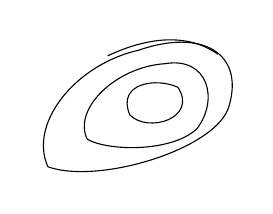
\begin{tikzpicture}
\draw (0,0) .. controls (-0.25,0.55) and (0.35,1.30) .. (1.15,1.48)
 .. controls (1.95,1.76) and (2.50,1.45) .. (2.30,0.77)
 .. controls (2.15,0.23) and (0.65,-0.23) .. (0,0);
\draw (0.50,0.35) .. controls (0.31,0.73) and (0.86,1.27) .. (1.49,1.31)
 .. controls (2.03,1.40) and (2.18,0.86) .. (1.89,0.48)
 .. controls (1.56,0.18) and (0.76,0.20) .. (0.50,0.35);
\draw (1.04,0.66) .. controls (0.87,1.06) and (1.37,1.14) .. (1.65,1.01)
 .. controls (1.91,0.62) and (1.27,0.42) .. (1.04,0.66);
\draw (0.76,1.41) .. controls (1.25,1.64) and (1.76,1.71) .. (2.16,1.43);
\end{tikzpicture}
\end{adjustbox}

$A$ — самосопр. опер. на мн-зии $X$.

$\Lambda\subset R$.
[Под $\Lambda$:] \underline{отрезок}.

\underline{В $E_\Lambda$ плотны содержащиеся там непрерывные ф-и.}

(требуется) — так для эл. опер.

$x_0\longrightarrow$ мера Планшереля на спектре $A$.
\begin{equation*}
M_{x_0}(\Lambda)=
\max_{\substack{f\text{-непр. в }E_\lambda,\ \|f\|=1\\
                 \text{(по всему }X\text{)}}}
|f(x_0)|^2.
\end{equation*}
\Unclear{GELFAND-P000283}{spectral-subscript}{[Под $\max$: $E_\lambda$; возможно, $E_\Lambda$.]}

[Справа:] Это мера (быть может, беск.)

\SourcePage{GELFAND-P000284}{53}
% Оригинал: images/GELFAND-P000284.png; 1984 x 2416; полный кадр просмотрен.
% Просмотр kernel-artin-top: bbox=(70,20,1950,630); увеличение=3x.
% Просмотр artin-answer: bbox=(80,565,1875,1075); увеличение=3x.
% Просмотр solution-parameter-symbols: bbox=(905,565,1280,725); увеличение=5x.
% Просмотр ficera-heading-and-body: bbox=(130,1080,1860,1590); увеличение=3x.
% Просмотр signorini-forces-and-diagram: bbox=(105,1575,1870,1955); увеличение=3x.
% Просмотр stress-equations-bottom: bbox=(120,1910,1775,2385); увеличение=3x.
% Просмотр cancelled-stress-equation: bbox=(735,2010,1275,2122); увеличение=5x.
% Просмотр boundary-force-and-normal: bbox=(260,2190,830,2375); увеличение=5x.
% Просмотр elastic-body-figure: bbox=(115,1235,515,1515); увеличение=4x.
% Просмотр detachment-figure: bbox=(1235,1665,1615,1905); увеличение=4x.
% Просмотр analytic-abbreviation-recheck: bbox=(150,1840,780,1940); увеличение=4x.
$K_\Lambda(x,y)$ — ядро $E_\Lambda$.

[Справа — вопросительный знак в кружке. Под строкой длинная разделительная линия с точкой посредине; правый конец линии заострён.]

[Вверху справа — 53, с линией слева и снизу.]

\underline{Каздан.} М. Артин в сем. Бурбаки.
\begin{equation*}
f_i(x_1,\ldots,x_n)=0,\qquad 1\leq i\leq k.
\end{equation*}
$f_i$ — сход. степ. ряды.

Когда сущ. реш. \Unclear{GELFAND-P000284}{artin-solution-parameters}{$\psi_j(t_1,\ldots,t_\tau)$ [буква функции: $\psi$ или $Y$; последний индекс: $\tau$ или $r$]}

\underline{Ответ:} тогда и только тогда, когда есть реш. в форм. степ. рядах.

(сколь угодно близко к формальному)

[Под скобкой:] достраивается

[Разделительная черта: — $\bullet$ —.]

\textbf{22.9.69г.}

\underline{Фикера об одностор. гран. задачах.}

[Рисунок слева:]
\begin{adjustbox}{max width=\linewidth}
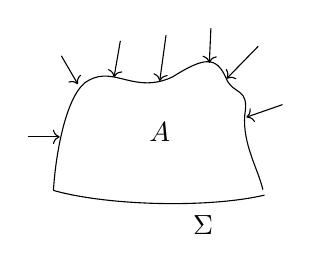
\begin{tikzpicture}
\draw (0,0.08) .. controls (0.03,0.57) and (0.17,1.34) .. (0.45,1.48)
 .. controls (0.78,1.66) and (1.03,1.30) .. (1.51,1.52)
 .. controls (1.91,1.77) and (2.07,1.80) .. (2.20,1.49)
 .. controls (2.29,1.29) and (2.49,1.39) .. (2.43,1.04)
 .. controls (2.40,0.67) and (2.60,0.35) .. (2.66,0.09);
\draw (0,0.08) .. controls (0.67,-0.11) and (1.94,-0.15) .. (2.68,0.02);
\draw[->] (-0.32,0.76) -- (0.08,0.76);
\draw[->] (0.10,1.79) -- (0.31,1.43);
\draw[->] (0.85,1.98) -- (0.77,1.52);
\draw[->] (1.43,2.05) -- (1.35,1.47);
\draw[->] (2.00,2.14) -- (1.98,1.70);
\draw[->] (2.60,1.91) -- (2.20,1.50);
\draw[->] (2.91,1.17) -- (2.45,1.01);
\node at (1.35,0.82) {$A$};
\node at (1.90,-0.36) {$\Sigma$};
\end{tikzpicture}
\end{adjustbox}

Эластичн. тело на пов. $\Sigma$ жёсткой и без трения.
И тензор напр. $\equiv0$.

$A$ — естеств. объём тела.

На своб. части границы сила $\varphi$ на $\partial A-\Sigma=\Sigma^*$.

[Под $\varphi$, с дугой к подписи:] плотность.

Внутри тоже нек-рые силы $f$ — объёмные.

Пусть тело перех. в полож. равн.

Оно может отойти от $\Sigma$.

\SourceFigure{GELFAND-P000284}{detachment-figure}{Справа от «Оно может отойти от $\Sigma$»: контур тела над наклонной опорной линией, с подъёмом нижней границы в середине; левое касание видно, точное правое касание или зазор неясны. Подписей и стрелок нет.}

Это аналит. задача (постановка A. Signorini, 1959)

$\sigma_{ik}$ — тензор напряжений.

Внутри тела

[Зачёркнуто: $(\sigma_{ik})_k-f_i=0$. Справа написано:]
\begin{equation*}
\sigma_{ik/k}-f_i=0.
\end{equation*}
$(\operatorname{div}\sigma=f)$.
\begin{equation*}
\sigma_{ik}\nu_k-\varphi_i=0.
\end{equation*}
— гран. условия.

($\nu$ — вект. нормали)

\SourcePage{GELFAND-P000285}{unlabelled}
% Оригинал: images/GELFAND-P000285.png; 1984 x 2416; полный кадр просмотрен.
% Просмотр contact-conditions-top: bbox=(75,25,1650,495); увеличение=3x.
% Просмотр free-surface: bbox=(175,495,1150,990); увеличение=3x.
% Просмотр elastic-potential: bbox=(180,955,1925,1345); увеличение=3x.
% Просмотр energy-functional: bbox=(205,1340,1460,1740); увеличение=3x.
% Просмотр minimum: bbox=(210,1680,1480,1960); увеличение=3x.
% Просмотр model-problem: bbox=(180,1950,1950,2408); увеличение=3x.
% Просмотр admissible-class-letter: bbox=(930,1540,1125,1690); увеличение=7x.
% Просмотр regularity-domain: bbox=(770,1660,960,1750); увеличение=8x.
% Просмотр ellipticity-indices: bbox=(665,2160,1240,2255); увеличение=5x.
% Просмотр boundary-partition-figure: bbox=(210,2130,540,2408); увеличение=4x.
[Сверху и по бокам выделено:] \underline{На $\Sigma$.}

$u_i$ — вектор смещения.

Условие
\begin{equation*}
u_i\nu_i=0\qquad(\text{на }\Sigma).
\end{equation*}
Норм. реакция
\begin{equation*}
\sigma_{ik}\nu_i\nu_k\geq0.
\end{equation*}
\begin{equation*}
\sigma_{ik}\nu_i\tau_k=0
\qquad\text{— танг. комп.}
\end{equation*}
[Условие и следующие формулы объединены ступенчатой линией, проходящей слева и снизу.]

В точке своб. поверхн:
\begin{equation*}
\begin{cases}
u_i\nu_i>0,\\
\sigma_{ik}\nu_i\nu_k=0,\\
\sigma_{ik}\nu_i\tau_k=0.
\end{cases}
\end{equation*}
\textbf{Но} неизвестно, где что.

Не учли ещё, что упругое тело.

\underline{$W(x,\varepsilon)$}
\qquad $\varepsilon=\{\varepsilon_{ik}\}$
\qquad $\varepsilon_{ik}=2^{-1}(u_{i/k}+u_{k/i})$

[Под $W(x,\varepsilon)$:] потенциал.

[Под формулами для $\varepsilon$:] Тенз. деформации.

Связь:
\begin{equation*}
\sigma_{ik}+W_{\varepsilon_{ik}}=0
\qquad\text{на }A.
\end{equation*}

Пробл. сущ. и единств.
\begin{equation*}
I(u)=\int_A W[x,\varepsilon(u)]\,dx
-\underbrace{\int_A f_i u_i\,dx}_{\text{работа }f}
-\underbrace{\int_\Sigma\varphi_i u_i\,d\Sigma}_{\text{работа }\varphi}.
\end{equation*}
(Энергия суммарная)

\Unclear{GELFAND-P000285}{energy-boundary-domain}{[В первом поверхностном интеграле написано $\Sigma$, не $\Sigma^*$.]}

\underline{В классе допуст. смещений} \Unclear{GELFAND-P000285}{admissible-class-letter}{$\mathcal W_\Sigma$ / $\mathcal U_\Sigma$}.

Если сущ. минимум в $C^1(\Sigma)$, то он решение.

обратно, решение — $\min$.

\Unclear{GELFAND-P000285}{regularity-domain}{[В источнике именно $C^1(\Sigma)$; область класса гладкости не уточнена.]}

Но: в этом классе \underline{$\min$} не сущ.

[Разделительная черта: — $\cdot$ —.]

\begin{equation*}
I(u)=\frac12\int_A a_{nk}(x)u_{/n}u_{/k}\,dx
-\int_A fu\,dx-\int_{\Sigma^*}\varphi u\,d\sigma.
\end{equation*}
\begin{equation*}
a_{nk}(x)\mu_n\mu_k\geq\rho_0\mu_n\mu_n.
\end{equation*}
\begin{equation*}
\mathcal U_\Sigma:\quad u|_\Sigma\geq0.
\end{equation*}
(Модельная задача)

\SourceFigure{GELFAND-P000285}{boundary-partition-figure}{Овальный контур с двумя отмеченными стыками; над верхней дугой $\Sigma^*$, слева от нижней — $\Sigma$. Правая отметка кольцевая; у левой неясен дополнительный косой штрих, поэтому стрелка не дорисована.}

\SourcePage{GELFAND-P000286}{54}
% Оригинал: images/GELFAND-P000286.png; 1984 x 2416; полный кадр просмотрен.
% Просмотр signorini-boundary-problem: bbox=(60,20,1905,370); увеличение=3x.
% Просмотр nonexistence: bbox=(100,310,1685,830); увеличение=3x.
% Просмотр artin-heading-and-references: bbox=(70,830,1790,1265); увеличение=3x.
% Просмотр analytic-system: bbox=(120,1245,1800,1645); увеличение=3x.
% Просмотр example-and-induction: bbox=(80,1595,1965,2000); увеличение=3x.
% Просмотр ring-reformulation: bbox=(105,1970,1960,2385); увеличение=3x.
% Просмотр boundary-derivative-symbol: bbox=(575,60,1015,190); увеличение=5x.
% Просмотр overwritten-integral-domain: bbox=(480,180,660,385); увеличение=6x.
% Просмотр soviet-authors: bbox=(520,990,1135,1095); увеличение=5x.
% Просмотр induction-abbreviation: bbox=(95,1855,465,1950); увеличение=5x.
% Просмотр parameter-last-index: bbox=(950,1410,1110,1530); увеличение=6x.
% Просмотр journal-number: bbox=(770,1070,920,1150); увеличение=7x.
% Просмотр unknown-functions-letter: bbox=(650,1410,945,1530); увеличение=5x.
% Просмотр integral-domain-lower-strokes: bbox=(575,300,640,385); увеличение=8x.
% Просмотр integral-domain-final-review: bbox=(475,290,585,395); увеличение=8x.
Отсюда получ. зад.
\begin{equation*}
u=0,\quad a\frac{\partial u}{\partial\lambda}\geq0
\qquad\text{или}\qquad
\begin{cases}
u>0,\\
a\dfrac{\partial u}{\partial\lambda}=0.
\end{cases}
\end{equation*}
[Первая пара условий многократно обведена; нижний край обводки заштрихован.]

[Справа, с линиями слева, снизу и справа:]
\begin{equation*}
(a_{nk}u_{/k})_{/n}=f.
\end{equation*}
[Вверху справа — 54, с линиями слева и снизу.]

Необходимо:
\begin{equation*}
\int_A f\,dx+\int_{\Sigma^*}\varphi\,d\Sigma\leq0.
\end{equation*}
\Unclear{GELFAND-P000286}{first-integral-differential}{[Дифференциал первого интеграла: $dx$ / $d\Sigma$; возможно, $\Sigma$ исправлена на $x$.]}

\Unclear{GELFAND-P000286}{first-integral-domain-overwrite}{[Под первым интегралом: $A$, написанное поверх зачёркнутого знака, возможно $\Sigma$.]}

Пусть $f\leq0$ на $A$ и $\varphi<0$ на $\Sigma^*$.

По принц. $\min$ $u$ не может иметь мин. в $A$.

Не имеет реш. в \underline{$C^1(\bar A)$}.

[Под строкой волнистая линия; слева к ней направлен короткий косой штрих со стрелкой.]

(выв. из ф-лы Грина)

\underline{сразу противоречие — получ. разрыв производной.}

[Снизу и по бокам выделено:] \textbf{29.9.69}

\underline{Каздан} \underline{Формулировка} рез. \underline{М. Артина}. (1968).

(в СССР независ. \Unclear{GELFAND-P000286}{pokorny-surname}{Покорний / Покорный} и Рыбкин)

УМН, т. 15, $N=4$ (1960) стр. 169

и Меламед

Сиб. мат. журнал

\begin{equation*}
f_i(x_1,\ldots,x_k)=0,\qquad 1\leq i\leq n.
\end{equation*}
набор. сход. степ. рядов (в окр. 0

Пытаемся найти
\begin{equation*}
x_j=x_j(y_1,\ldots,y_\ell),\qquad j=1,\ldots,k.
\end{equation*}
[Формула и условие на $j$ по отдельности выделены линиями слева, снизу и справа.]

чтобы рав-ва вып. при подстановке.

\underline{Достат. найти такие ф-и в форм. степ. рядах.}

[Под чертой, слева:] \underline{Пример.}
\begin{equation*}
x_1^2-x_2^3=0
\qquad
\begin{aligned}
x_1&=y^3,\\
x_2&=y^2.
\end{aligned}
\end{equation*}

[Справа, отделено вертикальной чертой и подчёркнуто снизу:]
Тогда найд. реш. в аналит. ф-ях, сколь угодно близкое.
(с люб. числом производных)

[Под общей чертой:]
зад. делается индукцией по числу $x_j$.

и более сложн. инд.

\underline{Переформул.}

Это ур-я аналит. мн-ва и 2 кольца
\begin{align*}
A&=C\{y_1,\ldots,y_\ell\} &&\text{сход. ряды.}\\
B&=C[[y_1,\ldots,y_\ell]] &&\text{форм. ряды.}
\end{align*}

Если [вставлено над строкой в обводке: у мн-зия] есть точка со знач. в $B$, то
есть точка и со знач. в $A$.

\SourcePage{GELFAND-P000287}{unlabelled}
Индукция и по связн. компонентам. (\underline{числу их})

Непривод. — подкусок имеет меньшую размерность.

1) \underline{Если для неприв. мн-зий док., то и всегда док.}
[Под «мн-зий»: (данной разм.); под «всегда док.»: (данн. разм.).]

Выб. ур-я, леж. в идеале,
\Unclear{GELFAND-P000287}{upper-cancelled-word}{[зачёркнуто: неразборчиво]}
соотв. этой компоненте.

\underline{Добавл. ур-ей.} Рассм. простой идеал.

\begin{adjustbox}{max width=\linewidth}
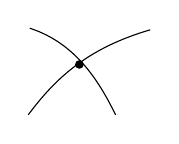
\begin{tikzpicture}[x=1cm,y=1cm]
\draw (0,0) .. controls (0.35,0.47) and (0.76,0.85) .. (1.55,1.08);
\draw (0.02,1.1) .. controls (0.64,0.90) and (0.93,0.36) .. (1.11,0);
\fill (0.65,0.64) circle (0.055);
\end{tikzpicture}
\end{adjustbox}
\Unclear{GELFAND-P000287}{ideal-letter}{$\mathcal{J}$}
$= (\underline{\text{Пересеч. простых}})$.

Получ. 2 сист. ур-й. $\forall$ решение удовл. \underline{одной из этих систем}.

(Если геом. точка леж. на
\Unclear{GELFAND-P000287}{middle-cancelled-word}{[зачёркнуто: неразборчиво]}
мн-зии, то она лежит на одной из компонент.)

\Unclear{GELFAND-P000287}{left-cancelled-mark}{[На левом поле зачёркнутый знак; неразборчиво.]}
Остальное — в следующий раз.

\underline{Л. Фаддеев.}

\underline{О результ. одного вычисл. эксперимента},
\Unclear{GELFAND-P000287}{title-cancelled-word}{[зачёркнуто: неразборчиво]}
\underline{им. отн. к прогр. Кириллова}
[Приписано ниже: \underline{опис. предст.}]

Представление — квантование класс. механики.

Примеры и пробл. о правилах квантования.

$M_{2n}$ — симпл. мн-зие, \Unclear{GELFAND-P000287}{form-abbreviation}{обл.} $\Omega$ — 2-формой (невырожд.).
$\Omega=d\omega$.

$d\mu=\Omega^n$ — мера.
\begin{equation*}
f\longrightarrow X_f\qquad (\text{по ф-ии поле})
\end{equation*}
\begin{equation*}
\underline{\Omega(X_f,Y)=Yf}
\end{equation*}
[Формула обведена снизу и с боков.]

Гамильтоновы поля $X_f$ образ. алгебру Ли
\begin{equation*}
[X_f,X_g]=X_{\{f,g\}},
\end{equation*}
где $\{f,g\}$ — скобки Пуассона (она этим определяется).

Опер. $X_f$ антисимм. в $L^2$ с мерой $d\mu=\Omega^n$.
(Она сохр. по теор. Лиувилля.)

Элем. алгебры Ли $X_f\longrightarrow$ отвечает опер. в $L^2$.

\underline{1951} Ван Хов нашёл 1-пар. сем-во представлений.
\begin{equation*}
Z_f=X_f+\alpha\bigl(\omega(X_f)-f\bigr)
\end{equation*}

\SourcePage{GELFAND-P000288}{55}
Тогда вып. условие представления
\begin{equation*}
\omega(X_f)-f=\ell_f
\end{equation*}
\underline{Утвержд. Ван-Хова:} Это снова предст., не эквив. ни при одном $\alpha$
\begin{equation*}
[Z_f,Z_g]=Z_{\{f,g\}}
\end{equation*}
Но это ещё не переход к квантовой механике, т. к. пока всё в пр-ве
\underline{всех переменных}, а не половины их.

Рассм. теперь $SO(3)$ с ест. предст. в $\mathbb{R}^3$.
На орбитах $(S^2)$ естеств. компл. структура.

Результат вычисления $Z_f$, когда $X_f$ — генер. группы вращ.

[Зачёркнуто: $X_1,X_2,X_3$.]
\begin{equation*}
x_1^2+x_2^2+x_3^2=a^2\quad\text{— орбита}
\end{equation*}
Функции $x_1,x_2,x_3$. Соотв. опер. Ван-Хова:

\begin{center}$\rule{1.5cm}{0.4pt}\quad\bullet\quad\rule{1.5cm}{0.4pt}$\end{center}

\underline{Зад. квантования.}

\begin{adjustbox}{max width=\linewidth}
\begin{tikzpicture}[x=1cm,y=1cm]
\draw[->] (-0.85,0) -- (1.2,0) node[right] {$q$};
\draw[->] (0,-0.55) -- (0,1.2) node[above left] {$p$};
\node at (1.65,0.75) {$\Omega=dp\wedge dq$};
\end{tikzpicture}
\end{adjustbox}

Гамильтониан $f=\dfrac{p^2}{2m}$ (своб. частица).
Надо ей сопост. оператор.

\begin{center}$\rule{1.5cm}{0.4pt}\quad\bullet\quad\rule{1.5cm}{0.4pt}$\end{center}

$f=x_1$.

\SourceFigure{GELFAND-P000288}{stereographic-diagram}{Рисунок к стереогр. проекции: замкнутый округлый контур над горизонтальной линией; четыре наклонных отрезка от его верхней области, проходящие через контур к линии и за него. Буквенных подписей нет.}

После стереогр. проекции (коорд. $z$) — \underline{$\omega$ не однозначна.}

\Unclear{GELFAND-P000288}{two-form-normalization}{$\displaystyle\Omega=a\frac{dz\wedge d\bar z}{(1+|z|^2)^2}$}
\begin{equation*}
X_i=X_f\quad\text{при }f=x_i
\end{equation*}
\begin{equation*}
\omega=\frac{a}{i}\frac{1}{1+z\bar z}(z\,d\bar z-\bar z\,dz)
\end{equation*}
На плоск. особ. нет, а особ. на $\infty$ (сев. полюс до проекции).
\begin{equation*}
X_1=\frac{1}{2i}\left((1-z^2)\frac{\partial}{\partial z}
 -(1-\bar z^2)\frac{\partial}{\partial\bar z}\right)
\end{equation*}
\begin{equation*}
Z_1=X_1+\frac{\alpha a}{2}(z+\bar z).
\end{equation*}
Аналит. и антианал. часть коммутируют!

Поэтому берём
\begin{equation*}
Y_1=\frac{1}{2i}(1-z^2)\frac{d}{dz}+\frac{\alpha a}{2}z
\end{equation*}
$Y_2,Y_3$ аналогично. Это базис алг. Ли, удовл. перест. соотн.

\SourcePage{GELFAND-P000289}{unlabelled}
Они дают предст. гр. вращений.

\underline{Мера, где они самосопр., сущ. лишь при целом $a$!}
\begin{equation*}
\frac{1}{(1+\bar z z)^a}
\end{equation*}
Квадр. интегрируемых — конечное число — полиномы.
Поэтому конечномерное представление.

\underline{След. раз:} Каждан;
(Шмид о $L^2$-когомологиях
(\Unclear{GELFAND-P000289}{announcement-name}{Везантин}, Рагунатан)).

\underline{Начнётся в $18^{30}$}. (\underline{конец} $20^{30}$)

\Unclear{GELFAND-P000289}{date-cancelled-sign}{[Перед датой зачёркнут знак.]}
$6/\mathrm{X}$-69 г.

\underline{\Unclear{GELFAND-P000289}{speaker-name}{Dusa mc Duff}}
\underline{О факторах типа $\mathrm{II}_1$.}

[Под именем: (по англ. и женщина).]

[На левом поле, вертикально: \underline{см. Наймарк.}]

Подкольцо кольца всех опер. в гильб. пр-ве наз. фактором,
если

1) \Unclear{GELFAND-P000289}{axiom-cancelled-sign}{[зачёркнуто: $\forall$?]}
$X\in M\Longrightarrow X^*\in M$.

2) $M$ слабо замкнут ($\forall$ посл. $X_n$ вход. слаб. предел).

3) Центр — из опер., кратных $I$.

\underline{Пример.} В кон.-мерном:
\begin{center}
\begin{adjustbox}{max width=\linewidth}
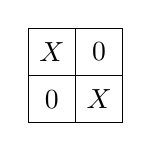
\begin{tikzpicture}[x=0.6cm,y=0.6cm]
\draw (0,0) rectangle (2,2);
\draw (1,0) -- (1,2);
\draw (0,1) -- (2,1);
\node at (0.5,1.5) {$X$};
\node at (1.5,1.5) {$0$};
\node at (0.5,0.5) {$0$};
\node at (1.5,0.5) {$X$};
\end{tikzpicture}
\end{adjustbox}
\end{center}

Всякий фактор в кон.-мерн. случае таков:

в $H_1\otimes H_2$ надо рассм. опер. $X\otimes1$ ($X$ — любой).

Вект. — матрица $\xi_{ik}$. Опер. — действ. на 1-ю координату.

\begin{center}$\rule{1.5cm}{0.4pt}\quad\bullet\quad\rule{1.5cm}{0.4pt}$\end{center}

Всякое слабо замкнутое кольцо (с инволюцией) разлаг. в прям. интеграл факторов.

Фон Нейман \underline{1935--36}.
[Над и под датой, а также справа от неё — горизонтальные черты.]

Пусть $M$ — фактор; тогда
$\dfrac{X+X^*}{2}$, $\dfrac{X-X^*}{2i}$ их порождают.

(самосопр.) $a=\int\lambda\,de_\lambda$, $e_\lambda\in$ фактору,
и порожд. фактор.

Фактор порожд. проекторами с $e^2=e$, $e^*=e$.

\SourcePage{GELFAND-P000290}{56}
Если \Unclear{GELFAND-P000290}{top-cancellation}{[зачёркнуто: неразборчиво]}
сущ. [вставлено над строкой: частичн.] изометрия из $M$, соед. подпр-ва,
соотв. проекторам, то 2 опер. наз. эквивалентными.
[Под «опер.»: (подпр.).]

Если отожд. эквив., то \underline{получится упорядоченность} (по включ.).

Классы экв. проекц. опер. можно складывать.

Отсюда можно измерять подпр-ва (сопост. числа подпр-ву).

(Акс. Архим. нет — $\infty$ есть).

\underline{Теор.} Если есть $\min$ подпр., то оно изом. кольцу всех опер.
в гильб. пр-ве.
\begin{equation*}
R=M\otimes M'\qquad(M'\text{ — коммут. фактор}).
\end{equation*}
Нет $\min\Longrightarrow$ или $\mathrm{II}_1$, $\mathrm{II}_{\infty}$ или $\mathrm{III}$.

$\mathrm{II}_1$ — никогда нет $\min$, но всё измер. числами из $(0,1]$
(есть $\max$) [приписано ниже: и акс. Архим.].

\underline{$\mathrm{II}_1$.}
\Unclear{GELFAND-P000290}{trace-cancelled-sign}{[зачёркнутый знак: $\forall$?]}
$\forall$ опер. имеет след и $\det$;
Верна minimax теория соб. знач.
(всё, что для матриц).
\begin{equation*}
\operatorname{Tr}(a)=\int\lambda\,d(\dim e_\lambda)
\qquad(\dim\text{ от }0\text{ до }1)
\end{equation*}

Само пр-во ещё не открыто.

Какие факт. типа $\mathrm{II}_1$?

1) гиперфинитный Муррей и Нейман — он один

2) Дж. Шварц

3) Ching

4) Sakai

5--6) Dixmier, Lance

7--8) Zeller-Meier

$7,8'$) Степин, Голодец

Континуум факторов $\Vert$ Dusa Mc Duff

\SourcePage{GELFAND-P000291}{unlabelled}
\underline{$13/\mathrm{X}$-69 г.}
\underline{След. раз Минлос и Синай.}

\underline{Гельфанд.}

\underline{О раб. Араки.}

\underline{Вопрос:} Пусть
\begin{equation*}
\begin{pmatrix}
\alpha(t)&\beta(t)\\
-\bar\beta(t)&\overline{\alpha(t)}
\end{pmatrix}
=u(t)\quad\text{унит. матр. с }\det1,
\qquad |\alpha(t)|^2+|\beta(t)|^2=1,
\qquad t\in[0,1].
\end{equation*}
Найти все неприв. унит. представления этой группы.
Это не сделано.

$\operatorname{supp}$ предст. $F$ — наим. замкн. мн-во, для к-рого вып. усл.
\begin{equation*}
u(t)\equiv1\quad\forall t\in U(F)\Longrightarrow T_{u(t)}=I
\end{equation*}
\underline{Задача:} сущ. ли неприв. унит. представл. с $\operatorname{supp}$ — отрезок.

\begin{center}$\rule{1.1cm}{0.4pt}\quad\bullet\quad\rule{1.1cm}{0.4pt}$\end{center}

$\operatorname{supp}$ — точка — оператор $u(t_0)$ (2-мерн. предст.).
Это предст. $\delta(t-t_0)$.

\Unclear{GELFAND-P000291}{representation-index}{$e:\ u(t)\longrightarrow T^e_{u(t_0)}\qquad\delta_e(t-t_0)$}

\begin{equation*}
u(t)\longrightarrow u(t_1)\otimes u(t_2)
\end{equation*}
неприв. предст. с $\operatorname{supp}$ — пара точек.

[Справа: (предст. по сути дела прям. суммы 2-х
\Unclear{GELFAND-P000291}{right-cancelled-word}{[зачёркнуто: матр.?]}
групп матр.).]

Можно $n$ точек.

Для счётн. мн-ва нельзя уже сделать (можно для сход. послед.).

\underline{Араки.}

Идея:
\begin{equation*}
e^K=\bigoplus_{n=0}^{\infty}S^n(K)
\end{equation*}
($K$ — гильб. пр-во)
\begin{equation*}
e^{\varphi}=\bigoplus_{n=0}^{\infty}\frac{1}{\sqrt{n!}}
\varphi\otimes\varphi\otimes\cdots\otimes\varphi
\end{equation*}
$\sqrt{n!}$, чтобы $(e^{\varphi},e^{\psi})=e^{(\varphi,\psi)}$.

$K\to e^K$ — функториальный переход
\begin{equation*}
K_1\oplus K_2\longrightarrow e^{K_1}\otimes e^{K_2}
\end{equation*}
В $\forall$ точке $t$ задаём представление в пр-ве $K(t)$ (напр. 2-мерном)
\begin{equation*}
\int_0^1 K(t)\,dt
\end{equation*}

\SourcePage{GELFAND-P000292}{57}
Рассм. $e^{\int_0^1 K(t)\,dt}$.

Получается в нём (из функт.) предст., к-рое приводимо.

\begin{center}$\rule{1.1cm}{0.4pt}\quad\bullet\quad\rule{1.1cm}{0.4pt}$\end{center}

Гр. матр. 1-го порядка $\alpha(t)=e^{x(t)}$.

Непр. предст.
\begin{equation*}
e^{x(t)}\longrightarrow C,\qquad
 e^{x_1(t)}e^{x_2(t)}\longrightarrow C_1C_2,
\qquad C=e^a
\end{equation*}
\begin{equation*}
x(t)\longrightarrow a
\end{equation*}
$a$ — лин. ф-л от \Unclear{GELFAND-P000292}{argument-case}{$X(t)$}
— обобщ. ф-я или распред.
\begin{equation*}
\delta(t-t_0):\qquad e^{x(t)}\longrightarrow e^{x(t_0)}
\end{equation*}
\begin{equation*}
x(t)\longrightarrow e^{\int_0^1 a(t)x(t)\,dt}
\end{equation*}
На окружности добав. усл. целочисленности.

\begin{center}$\rule{0.55cm}{0.4pt}\quad\bullet\quad\rule{0.55cm}{0.4pt}$\end{center}

Предст. здесь — обобщение распределения.

\SourcePage{GELFAND-P000293}{60}
\underline{17/XI-69 г.}\qquad \underline{Хьюитт.}

\underline{Один результат} (точный для всех \underline{комп.} групп)

[Под строкой: как для окружности.]

\Unclear{GELFAND-P000293}{upper-cancelled-sign}{[зачёркнуто: неразборчиво]}
\underline{Про $s$-числа:}

[Справа:]

\underline{Гантмахер;}

\underline{Wielandt}

\underline{Березин, Гельфанд}\qquad Труды \underline{М.М.О.} —

— \underline{$\forall$ полупр. группы Ли.}

из теор. предст. для компл. ф-и.

\underline{H. Weyl}\qquad \underline{и}\qquad \underline{Ky Fan.}

\Unclear{GELFAND-P000293}{middle-cancelled-sign}{[зачёркнуто: неразборчиво]}
Всё это для произв. группы и класса представлений:

\Unclear{GELFAND-P000293}{p-norm-formula}{
$\|\hat f\|_p=(\sum_{\sigma\in\Sigma}d_\sigma\|\hat f(\sigma\|_p^p)$}

\underline{Теор. Петера-Вейля — Планшереля}
\begin{equation*}
\|\hat f\|_2^2=\int_G |f|^2\,d\lambda;
\end{equation*}
\Unclear{GELFAND-P000293}{infinity-norm-subscript}{
$\displaystyle\|\hat f\|_\infty=\sup\{\|\hat f(\sigma)\|_{\mathfrak{S}_\infty}:\ \sigma\in\Sigma\}.$}
\underline{Лемма Рим.-Лебега:}
\begin{equation*}
\forall f\in L_1(G),\quad\forall\varepsilon>0\quad
\{\sigma:\ \|\hat f(\sigma)\|_{S_\infty}>\varepsilon\}
\end{equation*}
— конечное мн-во.

\underline{Т. Кунца.}\qquad $1<p<2$
\begin{equation*}
\|\hat f\|_{p'}\le\|f\|_p.
\end{equation*}
(Хаусд.-\Unclear{GELFAND-P000293}{young-abbreviation}{Юн.}).

\underline{Теор.} Харди-Литтлевуда — рав. лишь для $\underline{f(x)=\alpha e^{inx};}$

Для общ. группы всё не так просто: там для ф-й вида

$\chi$ — непр. ф-я на откр. подгруппе $G_0$,\quad
$\chi(e)=1$,\quad $\chi(xy)=\chi(x)\chi(y)$,

$\chi=0$ вне $G_0$.

Аналоги теорем Рисса-Торина есть.

\SourcePage{GELFAND-P000294}{unlabelled}
\underline{23.2.70 г.}

\underline{Каждан о раб. Гриффитса.}

\SourceFigure{GELFAND-P000294}{upper-left-sketch}{[Слева: овальный замкнутый контур с точкой внутри; сверху к нему подходят шесть длинных, преимущественно вертикальных кривых. У левого края контура имеются соединённые и повторные штрихи; их точная связность не установлена.]}

\begin{equation*}
T:\ H^i(V_s)\longrightarrow H^i(V_s)
\end{equation*}
(при обходе вокруг вык. точки)
\begin{equation*}
\exists N,\ \text{что}\quad (T^N-1)^{i+1}=0
\end{equation*}
\Unclear{GELFAND-P000294}{monodromy-qualification}{($T$ унипотентно).}

\begin{center}$\rule{1.1cm}{0.4pt}\quad\bullet\quad\rule{1.1cm}{0.4pt}$\end{center}

\begin{equation*}
\begin{adjustbox}{max width=\linewidth}
\begin{tikzcd}[row sep=small]
W\arrow[d]\\S
\end{tikzcd}
\end{adjustbox}
\end{equation*}
алгебраич. расслоение

база — 1-мерн. алг. мн-зие

(рим. пов. с выкол. точками).
\begin{equation*}
\pi_1(S):\ H^K(V_s)\longrightarrow H^K(V_s)\qquad(\text{коэфф. }C).
\end{equation*}
\underline{и опред. вект. расслоение}
\Unclear{GELFAND-P000294}{cancelled-bundle-sign}{[зачёркнуто: неразборчивый знак]}
(аналитическое)
\begin{equation*}
\begin{adjustbox}{max width=\linewidth}
\begin{tikzcd}[row sep=small]
E\arrow[d]\\S
\end{tikzcd}
\end{adjustbox}
\qquad O(E)\text{ — пучок ростков аналит. сеч.}
\end{equation*}
Есть канонич. связность из паралл. переносов на универс. накрывающей $\tilde S$.
(Там прям. произв.)

Будем изуч. вблизи выколотой точки.

Запишем связность в виде ур-я.
\begin{equation*}
\begin{array}{l}
f_1(z)\text{ — сечения}\\
\ldots\\
f_n(z)
\end{array}
\qquad (\text{базис в окр. }z).
\end{equation*}
Ур. Пикара-Фукса\qquad
\Unclear{GELFAND-P000294}{connection-operator}{$\dfrac{\partial}{\partial z}=A(z)$}

Перенесем $f_1(z)$ горизонт. в $z+\delta z$ и разложим по базису
\Unclear{GELFAND-P000294}{cancelled-basis-formula}{[зачёркнуто: $z+\delta z$, далее неразборчиво]}
$f_1(z+\delta z),\ldots$

Рассм. любое плоское сеч. расслоения.

оно удовл. ур-ю
\begin{equation*}
\frac{\partial}{\partial z}f(z)=A(z)f(z)
\end{equation*}
и все плоск. сеч. — решения этого ур-я.

\underline{Пример плоских сечений.}

Пусть \Unclear{GELFAND-P000294}{overwritten-cycle}{$\Phi_z$ [знак обведён либо исправлен]}
— цикл в слое ($K$-мерный).
\begin{equation*}
\Phi_z\subset V_z,\qquad \Phi_{z'}\subset V_{z'}.
\end{equation*}

\SourcePage{GELFAND-P000295}{62}
\Unclear{GELFAND-P000295}{pairing-index}{$((f_i(z),\phi_z))$}
— пример плоского сечения. —

[Справа под строкой: — вектор-ф-я.]

[Под формулой: знач. когом. на гом.]

\underline{Теор.} (Гриффитс)

$\exists$ такой базис $f_i(z)$, чтобы ур-е имело рег. особую точку,

т.е. $zA(z)$ голоморфно продолжается в $0$. (регулярно).

(Позв. судить о повед. периодов при прибл. к особой точке).

\underline{Следствие}

Рассм. любое плоск. сечение — реш. ур-я. Тогда оно разлаг. в ряд

\Unclear{GELFAND-P000295}{series-indices}{
$\displaystyle\sum_{n\le0}z^{n/N}
\big(\underline{C_{n0}}+\underline{C_{n1}}\ln z+\ldots+\underline{c_{nk}}\ln^k z\big)$}

\underline{Лемма}\qquad $\forall$ плоск. сеч. $\phi_z$

\Unclear{GELFAND-P000295}{bound-exponent}{$|\Phi_z|\le C|z|^{-a}|\ln z|^b$}

\begin{center}$\cdot\quad\cdot\quad\cdot\quad\cdot\quad\cdot\quad\cdot\quad\cdot\quad\cdot\quad\cdot\quad\cdot\quad\cdot\quad\cdot$\end{center}

\SourcePage{GELFAND-P000296}{unlabelled}
7/IX-1970 г.\qquad \underline{Семинар Гельфанда.}

\underline{Программа семинара.}

1. Каждан о связи формальной и алгебраич. геометрии.

2. Арнольд: Работы Гриффитса.

3. Митягин и Хенкин об их работах.

\Unclear{GELFAND-P000296}{cancelled-programme-number}{[зачёркнутый номер: 4.?]}
$1'$. Мойшезон о работах Артина.

?. $K$-теория конечных групп

[Справа: Браун, Тейт, Томсон, Суон, Кац.]

(Каждан, Бернштейн и т.д.)

4. Хиронака.

\underline{На след. семестр.}

$\zeta$-ф-я\qquad ($p$-адич. гарм. анализ).

Конечные группы.

\begin{center}$\rule{1.1cm}{0.4pt}\quad\bullet\quad\rule{1.1cm}{0.4pt}$\end{center}

\underline{Каждан.}

Где это изложено?

[Слева вертикально, у скобки, охватывающей пункты 1–4:
Когомологии афф. и проект. схем.]

1. Серр „Когер. алг. пучки”.

2. Более совр., но менее приятное\qquad Дьёдонне\qquad Мат. 9:1

3. Лекции Ю.И. Манина (часть 1)\qquad Алг. геометрия.

4. 3-й том Гротендика\qquad I.H.E.S., т.12

ч. \underline{III}, $N=1$.

\underline{Замеч. Гельфанда:} выуч. кн. Серра „Кон. группы” и „Гр. Ли и алг. Ли”.

(Входят в минимум по лин. алгебре)

[Справа стрелка вниз к приписке: $\downarrow$\quad 1 и 2-я часть.]

\underline{1-я часть:}\qquad Когомологии когерентных пучков.

[Последний заголовок подчёркнут пунктиром.]

§1. \underline{Определение схемы.}

Схема — окольцованное пр-во специального вида

Топ. пр-во, снабж. пучком колец. $O$\qquad (структ. пучок).

[Под «Топ. пр-во» — прямоугольная скобка с $X$.]

Аффинная схема.\qquad $A$ — комм. кольцо с 1.

$\operatorname{Spec}A$\qquad Точки — простые идеалы
\Unclear{GELFAND-P000296}{prime-ideal-symbol}{$\wp\subset A$}.

Топология: $\forall I\subset A$ сопост. мн-во простых идеалов $U_I\subset\operatorname{Spec}A$,

[Под $I$ вертикальная черта к слову «идеалу».]

сост. из прост. идеалов
\begin{equation*}
\wp\quad
\tikz[baseline=-0.4ex,x=1em,y=1em]{
\draw (0,0.25) .. controls (0.95,0.25) and (0.95,-0.25) .. (0,-0.25);
\draw (0.18,-0.45)--(0.50,0.45);
}
\quad I.
\end{equation*}
% Перечёркнутое включение воспроизведено без отсутствующей в источнике нижней черты.
Мн-ва $U_I$ наз. открытыми.
\SourcePage{GELFAND-P000297}{67}
\underline{Задача:} пров., что получ. топология.

Базис откр. множеств:
\begin{equation*}
f\in A\ \leadsto\ U_f\subset\operatorname{Spec} A\quad\text{из}\quad \mathfrak p\ \text{∌}\ f.
\end{equation*}
\underline{Задача:} $U_f$ — базис.

\underline{Задача:} вып. самая слабая акс. отделимости
(из 2-х точек 1 можно отд. окр.)

\underline{Локализация.}

Пусть $S$ — мультипл. мн-во в $A$, не содерж. $0$ (замкн. отн. умн.)

Кольцо $A_S$ сост. из пар $\dfrac a s$:
\begin{equation*}
\frac a s=\frac{a'}{s'}\ \Longleftrightarrow\ \exists s''\in S\qquad
s''(s'a-sa')=0.
\end{equation*}
\underline{Задача:} это соотн. эквивал.

Позднее это понадобится для модулей.

Структ. пучок на $\operatorname{Spec} A$:
\begin{equation*}
\Gamma(U_f,O)=A_{\substack{\{f^n\}\\ n\geq0}},\qquad S=\{f^n\}.
\end{equation*}
\underline{Напоминание.}

\underline{Опр. пучка.}

Предпучок и $\forall U\subset X$ и покр. $\{U_\alpha^*\}$ мн-ва $U$ точна послед.
\begin{equation*}
\{U_\alpha^*\}\subset U\qquad\left(\bigcup U_\alpha^*=U\right).
\end{equation*}
\begin{center}
\begin{adjustbox}{max width=\linewidth}
\begin{tikzcd}[column sep=large]
F(U) \arrow[r] &
\underbrace{\displaystyle\bigoplus_\alpha F(U_\alpha)}_{\text{произвед. мн-в}}
\arrow[r,shift left=1.5pt] \arrow[r,shift right=1.5pt] &
\displaystyle\bigoplus_{\alpha,\beta} F(U_\alpha\cap U_\beta).
\end{tikzcd}
\end{adjustbox}
\end{center}
\Unclear{GELFAND-P000297}{sheaf-product-sign}{[В последовательности написаны знаки $\bigoplus$; подпись: «произвед. мн-в».]}
\begin{equation*}
F(U_\alpha)\longrightarrow F(U_\alpha\cap U_\beta)
\end{equation*}
\Unclear{GELFAND-P000297}{restriction-corrections}{[Следующая строка, с исправленными индексами:] $F(U_\alpha)\longrightarrow F(U_\beta\cap U_\alpha)$ [в левом индексе возможно $\beta$; первоначальные штрихи неразборчивы].}

\underline{Вопрос:} почему это разные стрелки?

Точность:
\begin{equation*}
\operatorname{Im} i=\{\,\cdot\mid\varphi_1=\varphi_2\}.
\end{equation*}
Слой пучка (предп.) в т. $x$ и т. д.

\underline{Задача:} док., что $\forall$ предпучку $\exists$ пучок с теми же слоями
(и единств.)

\underline{Замечание:} для опр. пучка предпучок дост. знать на базе.

[Слева от надписи — две горизонтальные черты с точкой между ними.]
\begin{flushright}
\underline{Конец напоминания.}
\end{flushright}
\begin{equation*}
U_f\subset U_g\ \Longleftrightarrow\ \exists n:\quad f^m=gh.
\end{equation*}
\Unclear{GELFAND-P000297}{inclusion-correction}{[Знак между $U_f$ и $U_g$ густо исправлен; виден контур $\subset$, первоначальный знак не читается.]}
\Unclear{GELFAND-P000297}{exponent}{[Показатель у $f$ читается как $m$, возможно исправленное $n$; после $\exists$ написано $n$.]}

(Равнос. теор. о том, что $\bigcap$ всех пр. идеалов есть радикал)

\SourcePage{GELFAND-P000298}{unlabelled}
\begin{equation*}
A_{\{g^n\}}\longrightarrow A_{\{f^n\}}.
\end{equation*}
\begin{equation*}
\frac a g\longrightarrow\frac{ah}{f^m},\qquad
\frac a{g^k}\longrightarrow\frac{ah^k}{f^{mk}}.
\end{equation*}

\begin{center}— · —\end{center}

\underline{Предсхема:} окольцов. пр-во, лок. изом. афф. схеме.

[Слева дугообразная стрелка вниз от определения к задаче.]

\underline{Задача.} $\forall f\in A$, $(U_f,O)={}$ афф. схема

\underline{Произведение предсхем.}\qquad $\operatorname{Spec} A$, $\operatorname{Spec} B$
\begin{equation*}
\operatorname{Spec} A\times\operatorname{Spec} B=\operatorname{Spec}(A\otimes B)
\end{equation*}
\underline{Задача:} определить
\Unclear{GELFAND-P000298}{task-word}{опред. [возможно: произв.]}
двух предсхем.

[Справа, в рамке:]

\underline{пример.}\quad $(Z_2\text{ и }Z_3)$.

$\operatorname{Spec} Z_2\times\operatorname{Spec} Z_3$ —
— пустое мн-во.

[Горизонтальная черта. Слева в рамке:]

Импровиз. Кириллова

\begin{equation*}
\begin{array}{cc}
X,&Y\\
\Vert&\Vert\\
\bigcup X_\alpha&\bigcup Y_\beta
\end{array}
\qquad\text{— предсхемы}
\end{equation*}
в \Unclear{GELFAND-P000298}{union-index}{$\displaystyle\bigcup_\alpha(X_\alpha\times Y_\beta)$ [нижний индекс исправлен; возможно $*$].}

\begin{equation*}
\begin{array}{cc}
X_\alpha\times Y_\beta&X_{\alpha'}\times Y_{\beta'}\\[1em]
X_\alpha\cap X_{\alpha'}&Y_\beta\cap Y_{\beta'}\\
\Vert&\Vert\\
\bigcup X_\gamma&\bigcup Y_\delta
\end{array}
\end{equation*}
\Unclear{GELFAND-P000298}{gluing-y-corrections}{[Буквы $Y$ в $\bigcup Y_\beta$ и в $Y_\beta\cap Y_{\beta'}$ обведены с исправлениями; первоначальные буквы не отделяются от поздних штрихов.]}

\underline{Лемма:}
$X_\alpha\subset X_{\alpha'}$, $Y_\beta\subset Y_{\beta'}$
$\Rightarrow X_\alpha\times Y_\beta\subset X_{\alpha'}\times Y_{\beta'}$.

\underline{См. Серр.}

[Горизонтальная черта.]

\underline{Предсхема $X$} наз. схемой, если $\Delta\subset X*X$ замкнута.
\Unclear{GELFAND-P000298}{diagonal-product}{[Знак между $X$ и $X$ похож на звездочку, возможно обведенное $\times$.]}

\underline{Задача:} док., что афф. схема явл. схемой.

Пусть $X$ — произв. предсхема, $\mathcal F$ — пучок $\mathcal O$-модулей
над \Unclear{GELFAND-P000298}{lower-correction}{[зачеркнут неразборчивый знак, возможно $x$]} $X$.
Он наз. квазикогерентным, если он лок. изом.

\SourcePage{GELFAND-P000299}{68}
коядру отображения:
\begin{equation*}
\underbrace{O^R}_{\text{прям. суммы.}}\overset{\varphi}{\longrightarrow}O^T.
\end{equation*}
$S,T$ — произвольные мн-ва.
\Unclear{GELFAND-P000299}{presentation-exponent}{[Первый показатель в отображении похож на исправленное $R$; в следующей строке написано $S,T$.]}

\underline{Задача:} привести пример не квазикогер. пучка.

\underline{Теорема.} Пусть $A$ — комм. кольцо и $\operatorname{Spec} A$ — афф. сх.
Отобр. из катег. квазиког. пучков модулей
\begin{equation*}
\mathcal F\longrightarrow\Gamma(\operatorname{Spec} A,\mathcal F)
\end{equation*}
в катег. модулей есть изоморфизм.

Т. е. катег. к.-к. пучков мод. над афф. сх. $A$ изом.
катег. модулей над $A$.

(Модуль глоб. сечений.)

(Это равносильно тому, что для афф. пр-в когом. нулевые)
\Unclear{GELFAND-P000299}{cohomology-qualification}{[Степени когомологий в этой фразе не указаны.]}

Квазикогер. пучок модулей опред. своими глоб. сечениями.

$28/\overline{\underline{\mathrm{IX}}}$.

\underline{Прямой и обр. образ пучков.}
\begin{equation*}
X\overset f{\longrightarrow}Y,\qquad X,Y\text{ — топ. пр-ва,}
\end{equation*}
$\mathcal F$ — пучок на $X$,
\begin{equation*}
\Gamma(U,f_*\mathcal F):=\Gamma(f^{-1}(U),\mathcal F),\qquad U\subset Y
\end{equation*}
получается предпучок на $Y$.

\underline{Упражнение} (лёгкое) — этот предпучок явл. пучком

\underline{Пример:} если $Y$ — точка, то $f_*\mathcal F$ — группа сечений исх. пучка,

($f^{-1}(U)$ может быть и пусто, тогда мн-во сечений пусто).
\Unclear{GELFAND-P000299}{empty-sections}{[В источнике: «тогда мн-во сечений пусто».]}

\underline{Очень важное понятие.}
[Подчеркнуто волнистой чертой.]

\underline{Обратный образ.}
\begin{equation*}
X\overset f{\longrightarrow}Y
\end{equation*}
$\mathcal G$ — пучок на $Y$

\SourcePage{GELFAND-P000300}{unlabelled}
Пучок $f^*\mathcal G$ определяется так:

$\forall\mathcal F$ на $X$ справедливо равенство:
\begin{equation*}
\fbox{$\operatorname{Hom}(f^*\mathcal G,\mathcal F)=\operatorname{Hom}(\mathcal G,f_*\mathcal F)$}\quad{}^{1)}
\end{equation*}
[Под левым $\operatorname{Hom}$ вертикальный штрих к подписи:]

мн-во морфизмов над $X$

Т. е. $\forall$ пучка $\mathcal F$ задано вз.-однозн. отобр. этих мн-в,
согласованные при морфизмах $\mathcal F$ друг в друга.

(Изоморфизм функторов на кат. пучков).

\underline{Конструкция}, доказ. существование $f^*\mathcal G$

\Unclear{GELFAND-P000300}{cancelled-formula}{[Зачеркнуто короткое выражение: $F(U)$ / $\Gamma(U,\mathcal G)$?]}
\begin{equation*}
\Gamma(U,\overline{f^*\mathcal G})=
\underset{\substack{\longrightarrow\\ V\supset f(U)}}{\lim}\Gamma(V,\mathcal G)
\end{equation*}
\Unclear{GELFAND-P000300}{limit-variable}{[Первый аргумент последнего $\Gamma$ густо исправлен: $V$, возможно поверх $U$.]}

это рав-во опред. предпучок\qquad $(V\subset Y)$

\underline{Упражн.:} ассоц. с ним пучок есть обратный образ

[Следующий пример слева выделен фигурной скобкой и знаком «!».]

\underline{Пример.}
\begin{center}
\begin{adjustbox}{max width=\linewidth}
\begin{tikzpicture}
\node at (-0.8,0) {$X=$};
\fill (0,0) circle (1.5pt);
\fill (0.8,0) circle (1.5pt);
\draw (0,0.35) -- (0,0.72);
\node[left] at (0,0.58) {$\mathcal G$};
\draw (0.8,0.35) -- (0.8,0.72);
\node[right] at (0.8,0.6) {$\mathcal G$};
\node at (2.8,0) {$Y=$};
\fill (3.4,0) circle (1.5pt);
\draw (3.4,0.4) -- (3.4,1.05);
\node[right] at (3.4,0.88) {$\mathcal G$};
\end{tikzpicture}
\end{adjustbox}
\end{center}
Когда $U\subset X$ есть точка, то $\mathcal G$, $U=X$ — тоже $\mathcal G$.
\underline{Не пучок.}

[Горизонтальная черта со стрелкой на левом конце.]

1) Определение \underline{$\operatorname{Hom}$:}

Отобр. $\mathcal F_1\longrightarrow\mathcal F_2$ над $X$ наз.
\Unclear{GELFAND-P000300}{footnote-cancelled-word}{[зачеркнуто неразборчивое слово]}
набор отобр.
\begin{equation*}
\begin{aligned}
\varphi_U:\Gamma(U,\mathcal F_1)&\longrightarrow\\
&\longrightarrow\Gamma(U,\mathcal F_2)\\
&\forall U\subset X.
\end{aligned}
\end{equation*}
и коммут. с опер. ограничения. (Морфизм функторов)

\SourcePage{GELFAND-P000301}{69}
\Unclear{GELFAND-P000301}{cancelled-hom}{[Зачеркнуто, в рамке:] $\operatorname{Hom}(\overline G,\mathcal F)=\operatorname{Hom}(\overline G,\overline{\mathcal F})$ [положение черт над буквами не вполне ясно].}
— опред. пучка, отв. предпучку
\begin{equation*}
\underline{\operatorname{Hom}(\mathcal F,G)=\operatorname{Hom}(\overline{\mathcal F},G)}
\end{equation*}
\underline{$\overline{\mathcal F}$ — предпучок},\qquad
$\mathcal F$ — ассоциир. предпучок.
\Unclear{GELFAND-P000301}{associated-presheaf}{[В источнике повторено слово «предпучок».]}

$\overline{\mathcal F}\longrightarrow\mathcal F$ — должно быть задано отображение (предпучков)

[В рамке, с волнистым подчеркиванием:]

\fbox{Следующий раз пропускается.}

\underline{Напоминание, § 2.}

\underline{Когомологии.}
\begin{equation*}
\begin{array}{c||cc}
X\text{ — топ. пр-во},&H^i(\mathcal F),&\check H^i(\mathcal F).\\
\mathcal F\text{ — пучок}& *\ \underline{\text{общекатег.}}&\underline{\text{по Чеху.}}
\end{array}
\end{equation*}
[Слева от двух видов когомологий — двойная вертикальная черта.]

$H^i(\mathcal F)$ — произв. функтор от функтора сечений.

Рассм. категорию $C$ пучков аб. групп над пр-вом $X$

\underline{Лемма 1.} — это абелева категория.

Важны инъект. пучки.

\underline{Лемма 2.} Дост. много инъект. объектов
(люб. пучок вклад. в инъект. пучок).

Функтор\quad \underline{пучку} $\longrightarrow$ сечения над всем $X$.
\begin{equation*}
0\longrightarrow\Gamma(\mathcal F')\longrightarrow\Gamma(\mathcal F)\longrightarrow\Gamma(\mathcal F'')
\end{equation*}
$\Gamma$ — полуточн. функтор (слева) и т. к. много инъект. объектов,
то опр. производные функторы.

Пусть $X$ — топ. пр-во $\{U\}$ — базис топологии в $X$,
такой что
\begin{equation*}
\check H^i(\mathcal F,\{u_i\})=0,\qquad i>0.
\end{equation*}
Тогда когом. настоящие
\Unclear{GELFAND-P000301}{cancelled-bottom-word}{[зачеркнуто: выч.?]}
совп. с выч. по Чеху.

И можно счит. их в ацикл. покрытиях.

\SourceFigure{GELFAND-P000301}{margin-figure}{[Внизу слева небольшой наклонный рисунок: несколько четырехугольных контуров, внутренние треугольные и заштрихованные участки, короткие штрихи по краям. Подписи и возможное математическое значение не установлены; воспроизводить по оригиналу.]}

\SourcePage{GELFAND-P000302}{unlabelled}
\underline{Эллипт. сист. 2-го порядка} - \underline{на мн-зии}\quad \underline{без}

\underline{младш. членов.}\qquad Есть ли у неё решения?

У опер. Лапласа известно, что нет

Число реш. $(\bmod\,2)$.

В принципе \underline{$\max$} есть топология
(\underline{Зад. Дирихле имеет 0-е решение})

[Разделительная черта.]

\underline{Каждан} об одной конкр. работе.

$G$ — компл. полупр. группа $(A_n\text{ или }D_n)$.

Рег. элем. — если централизатор ранга \underline{$n-1$}.

Субрегул. — если $\dim$ централизатора \underline{$n-2$},

(два совпад. соб. знач.)
\Unclear{GELFAND-P000302}{centralizer-ranks}{[В источнике подчеркнуто $n-1$ и $n-2$; знаки и формулировки «ранга» / «$\dim$» сохранены.]}

Рассм.
\begin{equation*}
G\overset{\varphi}{\longrightarrow}H/W
\qquad
\begin{array}{l}
(W\text{ — гр. Вейля}\\
\phantom{(}H\text{ — карт. подгруппа})
\end{array}
\end{equation*}
Элем. \Unclear{GELFAND-P000302}{regular-cancellation}{[зачеркнуто начало слова: суб / не?]}регул.
$\Longleftrightarrow$ отобр. регул. на нём.

$12/\overline{\underline{\mathrm X}}$.
\underline{Гипотеза Рота.}
[Над именем, в заостренной рамке: Rota.]
\underline{Фикс. конечное поле $F_q$.}

Пусть дано $\ell$ и $k>\ell$. Тогда $\exists N$ [над строкой вписано: такое], что если
разбить подпр-ва $\ell$-мерные в $N$-мерном подпр-ве,
\Unclear{GELFAND-P000302}{cancelled-conjunction}{[зачеркнуто: что?]}
то $\exists$ $k$-мерное, что все подпр-ва данного
$k$-мерного в один из классов войдут.
\begin{equation*}
F^N\supset E\qquad\dim E=k
\end{equation*}
и все его $\ell$-мерн. подпр. в одном классе.

\underline{Для $\ell=1$ доказана.}

Можно в проект. терминах (там прямая есть точка).

Если $P^N$ разб. на 2 кл., то есть прямая в одном классе.

\SourcePage{GELFAND-P000303}{70}
\underline{Каждан.}

\underline{Квазикогер. пучок} — пучок, лок. изом. коядру
отобр. своб. пучков.

\underline{Пример.} $A$ — кольцо, $M$ — модуль,
$\mathcal F_M$ — пучок модулей на $\underline{\operatorname{Spec}A}$.
\begin{equation*}
\underset{\substack{\text{мульт.}\\\text{сист.}}}{(S)\subset A}
\qquad M_S \qquad
\frac{m}{s}=\frac{m'}{s'}\quad\text{если }s''(s'm-sm')=0.
\end{equation*}
\begin{equation*}
M_f=M_{(f^n)}.
\end{equation*}
Сеч. на $U_f$ есть $M_f$.
\begin{equation*}
\Gamma(U_f,\mathcal F_M)=M_f.
\end{equation*}
Проверка предост. слушателям.

\underline{Лемма:} это пучок.

\underline{Другое опр. квазикогер. пучка.}

\underline{Опр. 2.} Квазиког. пучки — пучки, лок. изом. пучку вида $\mathcal F_M$.

\underline{Задача:} док. эквив. определений.

[Справа, за двумя вертикальными чертами, зачеркнута приписка:]
\Unclear{GELFAND-P000303}{cancelled-annotation}{изом. $M$?}

\underline{Осн. теорема.}

$\forall$ квазиког. пучок $\mathcal F$ на афф. схеме
[над строкой, в выноске: $\operatorname{Spec}A$]
имеет вид $\mathcal F_M$, где $M$ есть $A$-модуль.

\underline{Задача} (реш.)
\begin{equation*}
M=A^n\Rightarrow\mathcal F_M=\mathcal O^n,
\qquad
\begin{aligned}
A^m&\longrightarrow A^n\longrightarrow M\\
\mathcal O^m&\longrightarrow\mathcal O^n\longrightarrow\mathcal F_M.
\end{aligned}
\end{equation*}
В обр. сторону:
\begin{equation*}
\mathcal O^m\longrightarrow\mathcal O^n\longrightarrow\mathcal F
\quad\text{лок.}
\end{equation*}
\Unclear{GELFAND-P000303}{then-correction}{и? [исправлено]}
тогда сеч. $A^m\longrightarrow A^n\longrightarrow M$.

\underline{Док-во теоремы.}
\begin{equation*}
\mathcal F \qquad M=\Gamma(X,\mathcal F).
\end{equation*}
\begin{equation*}
\forall f\in A\qquad\Gamma(U_f,\mathcal F)=M_f.
\end{equation*}
$\forall$ афф. схема квазикомпактна (нет отделимости).
Из $\forall$ откр. покр. выб. конечное.

\SourcePage{GELFAND-P000304}{unlabelled}
\begin{equation*}
\mathcal F\vert_{U_{f_i}}=\mathcal F_{M_i},\qquad
M_i\quad A_{f_i}\text{-модуль}.
\end{equation*}
Сущ. естеств. отобр.
\begin{equation*}
\underline{M_f\longrightarrow\Gamma(U_f,\mathcal F)}.
\end{equation*}
[Отображение выделено снизу и с боков рамкой; выше — две черты и точка.]
\begin{equation*}
1/f\in\Gamma(U_f,\mathcal O_X),\qquad
\text{а }\mathcal F\text{ — пучок модулей.}
\end{equation*}

\begin{center}— · —\end{center}

\underline{Томсон}\qquad\underline{в изл. Гельфанда И. М.}

$(G,M)$ — пара.

$G$ — группа, $F_p=\overline{Z}/pZ$.
\Unclear{GELFAND-P000304}{field-bar}{Над первым $Z$ — отдельная горизонтальная черта.}

$M$ — модуль над $F_p$, и [вписано в выноске: точное неприв.]
предст. $G$ в $M$.

Треб., чтобы [зачеркнут знак:]
\Unclear{GELFAND-P000304}{generator-cancellation}{$M$?}
$G$ порожд. набором $\langle Q\rangle$, таких элем.:

[Зачеркнуто: если; над строкой в выноске вновь вписано: если]
$g\in Q$, то $M(g-1)^2=0$.

(\underline{Пример:} группа матриц порожд. элем. с жорд. клетками пор. 2).

Доказывается, что над кон. полем $F_p$ с $p>5$
$G$ может быть только классич. группой: $S$, $O$ и т. д.
(кроме $E_8$).
\Unclear{GELFAND-P000304}{classification-scope}{«классич. группой»; «кроме $E_8$» — так в записи.}

Остались хар-ки 2 и 3.

[Правее этой строки виден желтый значок примечания; текста примечания на скане нет.]

\begin{center}— · —\end{center}

\underline{Кириллов со слов Томсона.}

Ещё одна конечная пр. группа (\underline{Conway}) —

— не вход. ни в какую серию.

Гр. автоморфизмов

[Слева на поле: в. Далее зачеркнута строка:]
\Unclear{GELFAND-P000304}{lattice-cancellation}{$R^{24}\supset Z^{24}$?; далее неразборчивое зачеркнутое слово.}

[Справа:]
\begin{equation*}
R^{24}\supset\underset{\text{решётка}}{L}.
\end{equation*}
1) унимодулярная — фунд. обл. им. ед. объём.

2) [Зачеркнуто:]
\Unclear{GELFAND-P000304}{pairing-cancellation}{$(\lambda_i,\lambda_j)$ — целые.}
$(\lambda,\mu)$ всегда целое, а $(\lambda,\lambda)$ чётное.

\SourcePage{GELFAND-P000305}{71}
3) $\min(\lambda,\lambda)=4$.
\Unclear{GELFAND-P000305}{minimum-range}{Область минимума при $\min(\lambda,\lambda)$ не выписана.}

[Зачеркнуто:]
\Unclear{GELFAND-P000305}{top-cancellation}{4)?}
Такая реш. одн. опр. с точн. до автом.

[Между двумя горизонтальными линиями:]
Сигнатура дел. на 8 у полож. опр. форм.

\underline{Читать}
[ниже слева: \underline{по алг. геом.}; справа за двумя вертикальными чертами:]
1) Серр, 2) Манин 3) Дьёдонне
\Unclear{GELFAND-P000305}{book-number}{9:1?}

\underline{$19/\overline{\underline{\mathrm X}}$.}
\qquad\underline{И. М. Гельфанд.}

Пусть на $X$ дан пучок модулей.

$A$, $X=\operatorname{Spec}A$, $M$ — модуль,
$\mathcal F_M$ — соотв. пучок (пучковизация модуля $M$).

\underline{Пример не квазиког. пучка над $\operatorname{Spec}A$:}

слой $A$ в точке $x$ и $0$ в ост. точках.
[Строка подчеркнута волнистой линией.]
\begin{equation*}
\Gamma(U,\mathcal F)=
\begin{cases}
A&\text{если }x\in U,\\
0&\text{если }x\notin U.
\end{cases}
\end{equation*}
\Unclear{GELFAND-P000305}{section-variable}{Первый аргумент $\Gamma$ исправлен: $U$?}

\SourceFigure{GELFAND-P000305}{small-figure}{Справа от формулы — маленький четырехугольник с горизонтальной и вертикальной внутренними линиями; на вертикальной линии различим верхний наконечник, на правом конце горизонтальной — утолщение, похожее на наконечник. Верхний левый короткий штрих и точный состав линий требуют проверки. Подписей не видно.}

[На правом поле, в рамке с двойным штрихованным левым краем;
$m/f$ в кружке:]
\begin{equation*}
\frac{m}{f}\qquad fm=0.
\end{equation*}
\begin{equation*}
\frac{m}{f}=\frac{mf}{f^2}=0.
\end{equation*}

\underline{Пример} (И. Бернштейн).

$\mathbb C^n$, $I$ — идеал в кольце многочленов,
\Unclear{GELFAND-P000305}{ideal-letter}{Буква идеала: $I$ или $J$; в наборе $I$.}
ему соотв. подмн-зие [под этим словом: $M$],
$\dfrac{P}{Q}$ опр. во всех точках подмн-зия.

Тогда ему соотв. многочлен $R$, что
\begin{equation*}
\underline{\frac{P}{Q}=R\quad(\operatorname{mod}I)}\quad\text{(на нём)}.
\end{equation*}
[Правая приписка в двойной рамке:]
Более точн. теор.: если она локально такая.

\begin{equation*}
A=\mathbb C[x_1,\ldots,x_n],\qquad
\mathcal O_X\text{ — структ. пучок на }\underline{X=\operatorname{Spec}A}.
\end{equation*}
[Справа ниже:]
\begin{equation*}
\underline{\operatorname{Spec}A\supset\mathbb C^n}.
\end{equation*}
(не только на $\mathbb C^n$).

[Слева:]
\begin{equation*}
\underset{\underline{\text{подпучок}}}{\underline{I\subset\mathcal O}}
\end{equation*}
$I$ — идеал $(f_1,\ldots,f_n)$, модуль над $A$.

$\mathcal F_J$ — соотв. пучок, $\mathcal F_J\subset\mathcal O_X$.
\begin{equation*}
(I\subset A\Rightarrow\mathcal F_J\subset\mathcal F_A).
\end{equation*}

\SourcePage{GELFAND-P000306}{unlabelled}
\begin{equation*}
0\longrightarrow I\longrightarrow A\longrightarrow M\longrightarrow0,
\qquad\underline{M=A/I}.
\end{equation*}
\begin{equation*}
0\longrightarrow\mathcal F_I\longrightarrow\mathcal O_X
\longrightarrow\mathcal F_M\longrightarrow0.
\end{equation*}
\Unclear{GELFAND-P000306}{ideal-letter}{Буква идеала и соответствующего индекса: $I$ или $J$; в наборе $I$.}

[Зачеркнуто:]
\Unclear{GELFAND-P000306}{top-cancellation}{$\mathcal F_M$ — рац. ф-а?}

\underline{Сечения пучка $\mathcal F_M$:}

1) постр. по $M$

2) из точной послед.

Пусть $Y$ — мн-во нулей идеала $I$.

$P/Q$ — рац. ф-я, $Q\ne0$ на $Y$.
\begin{equation*}
P/Q\in\Gamma(X,\mathcal F_M)\qquad\text{из точности последовательности.}
\end{equation*}
Рассм. $X_Q$ [зачеркнут малый знак:]
\Unclear{GELFAND-P000306}{middle-cancellation}{неразборчиво}
и $X\setminus Y$.

[Под $X_Q$, с короткой соединительной чертой:]
\underline{здесь $P/Q$ в $\mathcal O_X$.}

Над $X\setminus Y$ рассм. сечение $\equiv0$.
\begin{equation*}
0\in\Gamma(X\setminus Y,\mathcal F_M).
\end{equation*}
\begin{equation*}
i\left(\frac{P}{Q}\right)\in\Gamma(X_Q,\mathcal F_M).
\end{equation*}
Строим сеч. пучка на $X$.

На пересечении они совпадают, т. к.
сеч. $\mathcal F_M$ на $X\setminus Y$ тожд. $0$,
т. к. $\mathcal F_M$ сосред. на $Y$.

Но! сеч. [вписано в выноске: этого] пучка есть элем. $M$ — многочлен.

[Слева перед следующей строкой зачеркнут знак:]
\Unclear{GELFAND-P000306}{lower-cancellation}{$\mathcal O$?}
\begin{equation*}
\underline{\mathcal O_X^I\longrightarrow\mathcal O_X^J}
\longrightarrow\mathcal F\longrightarrow0
\qquad U_f
\end{equation*}
[Под двумя первыми членами — короткие утолщенные скобки, соединенные нижней линией.]
\begin{equation*}
A^I\longrightarrow A^J\longrightarrow M\longrightarrow0.
\end{equation*}
\Unclear{GELFAND-P000306}{presentation-indices}{Верхние индексы прочитаны как $I,J$; первый без петли, второй с нижней петлей.}
\begin{center}
\fbox{$\mathcal F=\mathcal F_M$}
\end{center}
[У рамки заштрихованы боковые и нижний края.]

[Справа, за двумя вертикальными чертами:]
\underline{На дом:}
\SourcePage{GELFAND-P000307}{72}
\underline{Я. Синай.} Некоммут. теория вероятностей.

$H$ — конечномерное гильбертово. $\dim H=2$ уже нетрив.

$\ldots,H_{-1},H_0,H_1,H_2,\ldots$ с фикс. изом. на $H$ (базисом).

$I$ — конечное подмн-во, $H_I=\bigotimes_{i\in I}H_i$.
\Unclear{GELFAND-P000307}{tensor-rewritten}{Перед $H_i$ в произведении зачёркнут и переписан $H$-образный знак; прежняя запись неразборчива.}
Справа: $\dim H_I=2^k$, где $k=|I|$.

$\alpha(I)$ — алгебра матриц над $H_I$.
\Unclear{GELFAND-P000307}{cancelled-matrices}{После $H_I$ зачёркнуто короткое слово, похожее на «Всем».}

$I_1\subset I_2\Rightarrow\alpha(I_1)\subset\alpha(I_2)$.
Под включением: $(\ldots\otimes1)$.

Элем. $\alpha(I)$ — локальные наблюдения.

Замкнём $\bigcup\alpha(I)$ в равном. метрике.

$[-n,n]$.

$\alpha([-n,n])\subset\alpha([-n-1,n+1])$.

замкн. по норме (пополнение) (равном.).

Получ. алгебра $\underline{\alpha}$ квазилок. наблюдений. (с инвол.).

\underline{Теор. вероятн.} — $\Omega$ — пр-во (компактное), на $C(\Omega)$ полож. ф-лы (распр. вероятн.).

$\alpha$ игр. \underline{роль} $\underline{C(\Omega)}$.

Состояние $\varphi$ на $\alpha$
\Unclear{GELFAND-P000307}{state-rewritten}{После $\alpha$ зачёркнут $\varphi$-образный знак.}
— полож. нормир. ф-л (распр. вероятностей).

Справа: $\varphi(a)\ge0$ при $a\ge0$; $\varphi(e)=1$.

$\varphi(a^*)$ — вещ. при $a^*=a$.

1. Состояние типа меры.

Рассм. знач. ф-ла на $\alpha(I)$.

$\varphi(a)=\operatorname{tr}(\rho_I\cdot a)$, где $\rho_I\ge0$, $\operatorname{tr}\rho_I=1$.

Сост. типа меры — соб. вект. $\rho_I$ соглас. в след. смысле:

в $H_I$ сущ. базис $(e_1^{(i)},e_2^{(i)})$ — баз. в $H_i$ (зав. от $\varphi$).

$\underbrace{\bigotimes_{i_s\in I}e_{k_s}^{(i_s)}}$ — баз. в $H_I$.

\underline{Они — собст. в. для} $\rho_I$.

\SourcePage{GELFAND-P000308}{unlabelled}
$\varphi(\bigotimes e_{k_s}^{(i_s)})=\underline{\mu(k_1,\ldots,k_s)}$.
Справа: $\sum\mu(\ )=1$.
Под значением: распр. вероятн.

Мера на пр-ве послед., прин. знач. 1 и 2.

2. Состояния, порожд. гамильтонианом.

$A\in\alpha((0,1))$, $\underline{H(I)}$.

На $[-n,n]$ рассм. \fbox{$H_n=\sum_{i=-n}^{n-1}A_i$}.
$A_i$ — сдвинутое $A$.

$\displaystyle\varphi_n(a)=\frac{\operatorname{tr}e^{-\beta H_n}\cdot a}{\operatorname{tr}e^{-\beta H_n}}$.

$\underline{\varphi(a)=\lim_{n\to\infty}\varphi_n(a)\text{ сущ. }\forall A!}$

Это наз. сост, порожд. гамильтонианом $A$.

(из квантового распр. Гиббса)

Некоммут. аналог цепей Маркова.

Пусть $\varphi$ — состояние. Строится слабозамкн. кольцо опер. в гильб. пр-ве.

В алг. $\langle a_1,a_2\rangle=\varphi(a_2^*a_1)$.

Факториз. по идеалу $\ldots$

$H_\varphi$ — гильб. пр-во.

\Unclear{GELFAND-P000308}{cancelled-action}{Слева зачёркнуто $h\in H_\varphi$; мелкий индекс под зачёркиванием не вполне различим.}
$h\in H_\varphi\Rightarrow L_a=ah$.

Слабое замыкание — $M_\varphi$.

Когда оно фактор?

В основном типа 3.

\SourcePage{GELFAND-P000309}{73}
26/X. \underline{Каждан.}

\underline{Тривиальность когом. квазикогер. пучка на афф. схеме.}

$A^n$
\Unclear{GELFAND-P000309}{cancelled-affine}{Между $A^n$ и $\operatorname{Spec}$ зачёркнут знак, похожий на $=$.}
$\operatorname{Spec}\mathbb C[x_1,\ldots,x_n]$.
Справа: $\underline{(A^n\text{ — пр-во макс. идеалов})}$.

[Стрелка вниз от $A^n$ к $X$. Вставка «замкн.» над следующим словом, обведена и соединена с ним.]
$X$ — подмн-зие (алг.).

$Q|_X\ne0$, тогда $P/Q$ — ф-я на $X$, $\forall P$.

Тогда $\exists R$ — многочлен, $(\forall P\exists R)$:
$\displaystyle\left.\frac P Q\right|_X=R|_X$.

Рассм. идеал, соотв. $X$ (0 на $X$),
$F_1,\ldots,F_k$ — базис этого идеала.

Тогда $(F_1,\ldots,F_k,Q)=k[x_1,\ldots,x_n]$.

\Unclear{GELFAND-P000309}{cancelled-parenthesis}{Перед скобкой зачёркнут короткий $H$- или $R$-образный знак.}
(этот идеал не содержится ни в одном максимальном

$\exists$ полиномы $L_0,\ldots,L_k$.

$L_0Q+L_1F_1+\ldots+L_kF_k=P$;

Отсюда можно взять $R=L_0$.

(Теор. Гильберта — описание макс. идеалов)

Это док-во аналог. док-ву трив. когомологий
(это трив. 1-мерных когомологий).

$X=\operatorname{Spec}A$, $A$
\Unclear{GELFAND-P000309}{cancelled-ideal}{Перед $(f_1,\ldots,f_n)$ знак $=$ густо зачёркнут; под штрихами видна дополнительная наклонная черта.}
$(f_1,\ldots,f_n)$.

Рассм. $X_i=X_{f_i}$.

$A=(f_1,\ldots,f_n)\Leftrightarrow X=\bigcup X_i$.

Пусть $M$ — $A$-модуль, $\mathcal F_M$ — соотв. пучок.

\underline{Комплекс Чеха:}

$q$-цепь: $\forall$ набора инд. $1\le i_0,<\ldots,i_q\le n$ зад.
\Unclear{GELFAND-P000309}{chain-order-sign}{Непосредственно после $i_0$ видна отдельная запятая; следующие два густо переписанных знака перед многоточием не разрешены, кандидат — $<$. Запятая сохранена.}

$\displaystyle m_{i_0\ldots i_q}\in\Gamma(X_{i_0}\cap\ldots\cap X_{i_q},\mathcal F_M)=$

$=M_{f_{i_0}\ldots f_{i_q}}$.

\SourcePage{GELFAND-P000310}{unlabelled}
$\displaystyle(dm)_{i_0\ldots i_q}=\sum_{0\le j\le q+1}(-1)^j m_{i_0\ldots\widehat{i_j}\ldots i_{q+1}}$.

$d:C^q\longrightarrow C^{q+1}$.

$d^2=0$ и когом. гр. комплекс Чеха $C^*(M,\{f_i\})$.
\Unclear{GELFAND-P000310}{cancelled-module}{После $M$ в $C^*(M,\{f_i\})$ зачёркнута высокая петлеобразная буква.}

[Под $C^*$ дуга к подписи:]
кососимм. коцепи — $C(M,\{f_i\})$ (подпространство).

\underline{Предл.:} когомологии совп. (изом. индуц. вложением).

Для удобства — иногда $C^*$, иногда $C$.

\underline{Теорема:} $H^q(\{X_i\};\mathcal F_M)=0$ при $q\ne0$.

\underline{Док-во:} Пусть $m_{i_0\ldots i_q}\in M_{f_{i_0}\ldots f_{i_q}}$ — циклы.

[Горизонтальная черта.]

Там было $A=(f_1,\ldots,f_n,Q)$,

$m_{i_0i_1}\in M_{f_{i_0}f_{i_1}}$,

$(dm)_{i_0i_1i_2}=m_{i_0i_1}-m_{i_0i_2}+m_{i_1i_2}=0$.

Надо док.:
\Unclear{GELFAND-P000310}{coboundary-indices}{$\exists n_i\in M_{f_i}:\quad m_{i_ki_\ell}=n_{i_k}-n_{i_\ell}$. Буква перед $i$ и малые индексы у $m$ переписаны; чтение не окончательное.}

\underline{Упр.:} $(M_f)_g=M_{fg}$.

\Unclear{GELFAND-P000310}{cancelled-sum}{Зачёркнуто $\sum L_{ijk}f_if_jf_k(=1)$; мелкие индексы под зачёркиванием различимы не полностью.}

$m_{1,i}=n_1-n_i$.

Положим $n_1=0$,
\Unclear{GELFAND-P000310}{cancelled-choice}{Перед подчеркнутым $n_i=-m_{1,i}$ зачёркнут короткий $m$-образный знак.}
$\underbrace{n_i=-m_{1,i}}$, $\underline{i>1}$.

Неверно, т.к. $m_{1,i}$ им. вид
$\displaystyle\frac m{f_1^k f_i^\ell}$,

$\displaystyle\frac m{f_2 f_i^\ell}$,

$\vdots$

\underline{и скомбинировать, используя то, что это покрытие.}

\SourcePage{GELFAND-P000311}{74}
\Unclear{GELFAND-P000311}{cancelled-start}{В начале зачёркнуто «Рассм.»; средние буквы закрыты несколькими штрихами.}
Пусть для простоты $q=1$.

Даны $m_{i_0i_1}$
\Unclear{GELFAND-P000311}{cycle-sign}{Перед $m_{i_0i_2}$ густо переписан знак; видны две горизонтальные черты, кандидат — минус.}
$m_{i_0i_2}+m_{i_1i_2}=0$. $1\le i_k\le n$.

Надо найти $n_i\in M_{f_i}$: $m_{i_0i_1}=n_{i_0}-n_{i_1}$.

$m_{i_0i_1}=$
\Unclear{GELFAND-P000311}{cancelled-fraction}{Зачёркнутая дробь, похожая на $\bar m/f_{i_0}$; штрихи пересекают числитель и дробную черту.}
$\displaystyle\frac{\bar m_{i_0i_1}}{f_{i_0}^N f_{i_1}^N}$, $\bar m\in M$.

Найдём $L_i\in X_i$; $\sum L_if_i^N=1$.

Определим
\Unclear{GELFAND-P000311}{new-chain-indices}{$\displaystyle\bar n_{i_0}=\sum_{i_1}L_{i_1}\bar m_{i_0i_1}/f_{i_0}^N\in M_{f_{i_0}}$. Цифры у индекса суммы и у $L$ густо переписаны; кандидат — 1, также видны штрихи, похожие на 2.}

\begin{align*}
\bar n_{i_0}-\bar n_{i_1}
 &=\sum_i\left(\frac{L_i}{f_{i_0}^N}\bar m_{i_0i}-\frac{L_i}{f_{i_1}^N}\bar m_{i_1i}\right)=\\
 &=\frac1{f_{i_0}^N f_{i_1}^N}\sum L_if_i^N\left(\frac{\bar m_{i_0i}}{f_{i_0}^N f_i^N}-\frac{\bar m_{i_1i}}{f_{i_1}^N f_i^N}\right)=
\end{align*}
\Unclear{GELFAND-P000311}{chain-calculation}{В первой строке последний индекс у $\bar m_{i_0i}$ переписан. Перед следующим знаком $=$ зачёркнута маленькая запись. Под разностью во второй строке длинная угловая скоба без подписи; под последней разностью дуга с подписью $m_{i_0i_1}$.}

$=\sum L_if_i^N\underbrace{(m_{i_0i}-m_{i_1i})}_{m_{i_0i_1}}=m_{i_0i_1}$.

Это ещё не всё, т.к. рав-во в смысле кручёного
\Incomplete{GELFAND-P000311}{cancelled-word-loss}{После «кручёного» зачёркнуто короткое слово; его текст не восстановлен.}
\Unclear{GELFAND-P000311}{localization-cancellation}{Ниже зачёркнуто $M_{f_{i_0}^N\ldots f_{i_n}^N}$; конечный индекс старой записи неясен. Справа новая запись $M_{f_1^N\ldots f_n^N}$ под скобой.}
модуля, (точнее, в смысле $\underbrace{M_{f_1^N\ldots f_n^N}}$)

Рав-во: $\bar n_{i_0}-\bar n_{i_1}=m_{i_0i_1}$ справ., если его умн. на нек-рую степень.

\underline{Док-во Бернштейна:} пусть все $m_{i_0i_1}$ не сод. $f_{i_0}$ в знамен.
\Unclear{GELFAND-P000311}{bernstein-denominator}{Индексы у $m$ в условии Бернштейна густо переписаны; кандидат — $i_0i_1$.}
и рав-ва 0 не треб. умн. на $f_{i_0}$. Тогда всё проходит. Следствие:

$f_{i_0}^N m_{i_0i_1}$ — граница. То же для $f_{i_1}^N$ и т.д.

Справа: Когом. — модуль.

Т.к. $(f_{i_0}^N,\ldots,f_{i_n}^N)=1$, то всё в пор.

\SourcePage{GELFAND-P000312}{unlabelled}
\Unclear{GELFAND-P000312}{cancelled-heading}{Сверху зачёркнуто «Пусть $\varphi$»; после слова высокая вертикальная черта с коротким поперечным штрихом.}
[Две короткие горизонтальные черты.]

\underline{Синай.} $H_i$ — 2-мерное, $-\infty<i<+\infty$.

$I=$ любое конечное мн-во.

$H_I=\bigoplus_{i\in I}H_i$;
базис
\Unclear{GELFAND-P000312}{tensor-basis}{$\underbrace{\bigotimes e_{t_n}^{i}}$; малый индекс под $e$ не вполне различим, похож на $t_n$.}

$\alpha(I)$ — все матр. в $H_I$.

В $\alpha(I)$ ввод. норма опер. в гильб. пр-ве.

$I\subset I_1\Rightarrow\alpha(I)\subset\alpha(I_1)$ $(\otimes1)$.

$\alpha(I_1)=\alpha(I)\otimes\alpha(I_1\setminus I)$.

Получится нормир. кольцо (пополнение) $\alpha$.
(алгебра квазилок. наблюдений).

\underline{Новые операторы добавл.:}

$\varphi(a)$ — функционал (лин.), $\varphi(a)\ge0$ $\forall$ полож. матр. $a$.

В $\alpha(I)$ будет $\varphi(a)=\operatorname{Sp}(a\rho)=\operatorname{Tr}(a\rho)$.

$\underline{\varphi(a)\ge0}\Leftrightarrow\rho\ge0$.

$\underline{\varphi(e)=1}$ — некоммут. аналог распр. вероятностей;
состояние в к.т.п.

$\alpha(I)$ — кольцо матриц
\Unclear{GELFAND-P000312}{cancelled-matrix-word}{После «матриц» зачёркнуто короткое слово, похожее на «на».}
$\underline{\varphi(a)=\operatorname{Tr}(a\rho_I)}$,
$\underline{\operatorname{Sp}\rho_I=1}$.

На $\rho_I$ усл. согласования:

$\operatorname{Tr}_{I_1-I}(\rho_{I_1})=\rho_I$.

$\alpha(I_1)=\alpha(I)\otimes\alpha(I_1-I)$.

\underline{$\varphi$ — сост. типа меры.} $\longrightarrow$
\Unclear{GELFAND-P000312}{cancelled-measure-condition}{Справа зачёркнуто «пусть $\rho_i$ соотв. точке;». Следующей строкой зачёркнуто «тогда требуется $\rho_i\rho_j=\rho_j\rho_i$», индексы под густыми штрихами не вполне различимы. Внизу слева отдельно зачёркнуты две $\rho$-образные буквы с малыми индексами.}

если $\rho_I$ при различных $I$ коммутируют (в более широком пр-ве).

(одноточечные $\rho_i$ и $\rho_j$ всегда коммутир.).

\SourcePage{GELFAND-P000313}{75}
$\rho_i$ — матрица в $H_i$.

Пусть $e_1^i,e_2^i$ — базис из соб. векторов $\rho_i$,

$e_{\alpha_1}^{i_1}\otimes e_{\alpha_2}^{i_2}\otimes\ldots\otimes e_{\alpha_n}^{i_n}$.

Тогда $\rho(I)$ в нём диагон., т.к. перестан. со всеми $\rho_i$ (если некр. спектр то очев.) ($\exists$ такой базис).

$2^{|I|}$ соб. векторов $\mu(\alpha_1,\ldots,\alpha_n)$ — соб. значение.

Он характ. распр. типа меры. На него усл. согласов.:

$\sum_{\alpha_n}\mu(\alpha_1,\ldots,\alpha_n)=\mu(\alpha_1,\ldots,\alpha_{n-1})$ и т.д.

Рассм. беск. послед. 0 и 1.

$\ldots,\varepsilon_{-n},\varepsilon_{-n+1},\ldots,\varepsilon_0,\ldots$

группа (слож. mod 2). Мера опр. на цилиндрич. мн-вах $\alpha_1,\ldots,\alpha_n$ — фиксир. $\mu(\alpha_1,\ldots,\alpha_n)$.

Условие — согласованность этих мер.

$\prod\mathbb Z_2^i$. Можно меру Хаара.

\Unclear{GELFAND-P000313}{cancelled-pairing}{Перед $(a,b)$ зачёркнута $\varphi$-образная буква; петля перекрыта косыми штрихами.}
$\underbrace{(a,b)=\varphi(b^*a)}$.

$(a,a)=\varphi(a^*a)\ge0$.

Теперь факторизуем и пополним — гильб. пр-во.

$x a=X_a$ — лин. опер. — непр. в этом скал. произв.

Наше кольцо — лин. опер.

(см. дополнение к кн. Гельфанд, Шилов, Райков)

(Наймарк и др.)

Кольцо, порожд. состоянием $\varphi$.

Факторы типа 3. — они важны — это сдвиги.

\SourcePage{GELFAND-P000314}{unlabelled}
2/XI. \underline{И.М. Гельфанд.}

Рез. докладчика и В. Пономарёва (не мехматского).

[На верхнем поле жёлтый значок примечания с тремя чёрными горизонтальными полосами; текста внутри не видно.]

$P$ — кон-мерное пр-во, $E_1,\ldots,E_4$ — 4 подпр-ва (порядок важен).

$S=\{P;E_1,E_2,E_3,E_4\}$.

Это категория (морф. — перев. внутрь).

Эквив. изуч. катег. диаграмм
\SourceFigure{GELFAND-P000314}{quiver}{Четыре короткие стрелки сходятся внутрь к тесному центральному узлу: из верхнего правого, правого, нижнего и нижнего левого концов. На концах маленькие округлые отметки; центральные наконечники наложены друг на друга. Подписей не видно.}
в кат. кон-мерных пр-в.

Методы дают инф. о модулях и подмодулях.

$S\sim S'$, если $\exists$ лин. изом.

Прям. сумма ест. вводится.

Действует гр. подстановок.

Пример $E$; $A:E\to E$. График $\{(x,Ax)\}\subset E\oplus E$.

$A$ — график, $P=E\oplus E$, $E_3$ — график $A$.

Для описания сист. $E\oplus E$ надо задать

$E_1=E\oplus0$, $E_2=0\oplus E$ и диагональ $E_4=\{(x,x)\}$.

Пары
\Incomplete{GELFAND-P000314}{cancelled-pair-loss}{После «Пары» перед высоким петлеобразным штрихом зачёркнуто несколько букв; их текст не восстановлен.}
\Unclear{GELFAND-P000314}{cancelled-pair}{В конце зачёркнутой записи после «Пары» виден высокий $\varphi$- или $b$-образный штрих; чтение этого знака не окончательное.}
отобр.

$A:E\longrightarrow F$,

$B:F\longrightarrow E$.
\Unclear{GELFAND-P000314}{pair-spaces}{Буквы пр-в у начал обеих стрелок густо переписаны; конечное чтение $A:E\to F$, $B:F\to E$, прежние буквы неразборчивы.}
Справа: (Зад.

тоже описываются.

Зад. Кронекера — в ту же сторону.

Отношение — любой график.

\underline{Инварианты:}

4 прямых.

\begin{adjustbox}{max width=\linewidth}
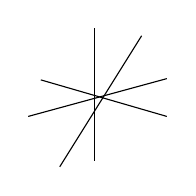
\begin{tikzpicture}[scale=0.8]
\draw (0,-1.0)--(0,1.1);
\draw (-0.55,-1.1)--(0.75,0.98);
\draw (-1.05,-0.3)--(1.15,0.3);
\draw (-0.85,0.28)--(1.15,-0.3);
\end{tikzpicture}
\end{adjustbox}

Инвар. — число $\lambda$ (одно).

2 — оси коорд.

3-е диагон.

4-е — график — $y=\lambda x$.

Меняем номера: $\lambda\to1-\lambda$, $\lambda^{-1}$, $\lambda/(\lambda-1)$.

Результат (док-во длинное).

\SourcePage{GELFAND-P000315}{76}
\Incomplete{GELFAND-P000315}{cancelled-start}{Слева перед «Пусть» зачёркнуто несколько букв, с большой округлой конечной петлёй; текст этой отменённой записи не восстановлен.}
Пусть дано $P,E_1,E_2,E_3,E_4$, тогда
\Unclear{GELFAND-P000315}{cancelled-system}{После «тогда» зачёркнуто «сист.»; сверху вставлено «сист.». Средние штрихи отменённого слова густые.}
сист. разлож. в прямую сумму след. образований

системы с деф. $0,\pm1,\pm2$.

\Unclear{GELFAND-P000315}{defect-symbol}{$\rho(S)=0,\pm1,\pm2$. Справа под угловой рамкой: $n(S)=\dim P$, $\rho(S)=2\dim P-\sum_{i=1}^4\dim E_i$, «дефект». Обозначение дефекта имеет петлю и нижний хвост; чтение $\rho$ или $g$ не окончательное.}

\underline{Неприводимые} (не разлож. в прям. сумму)

1) при $n(S)=2k$.

Баз. в $P$ $\{e_1\ldots e_k\ f_1\ldots f_k\}$.

$E_1=\{(e_1,\ldots,e_k)\}$.

$E_2=\{(f_1,\ldots,f_k)\}$.

$E_3=\{e_2+f_1,\ldots,e_k+f_{k-1}\}$.
\Unclear{GELFAND-P000315}{series-three-rewritten}{Сразу после левой фигурной скобки у $E_3$ зачёркнут узкий высокий знак. Последнее $e_k$ густо переписано; прежние штрихи неразборчивы.}

$E_4=\{e_1+f_1,\ldots,e_k+f_k\}$.

[Справа длинная фигурная скобка охватывает четыре строки, подпись $S_3(2k,-1)$. Горизонтальная черта.]

2) $\underline{S_3(2k,1)}$.

$E_1=(e_1,\ldots,e_k)$.

$E_2=(f_1,\ldots,f_k)$.

$E_3=(e_1,e_2+f_1,\ldots,e_k+f_{k-1},f_k\}$.

$E_4=\{e_1+f_1,\ldots,e_k+f_k\}$.

3) $E_1$, $E_2$ — те же.

Справа под угловой рамкой: $S_{13}(2k,0)$.

$E_3=\{e_1,e_2+f_1,\ldots,e_k+f_{k-1}\}$.
\Unclear{GELFAND-P000315}{series-zero-rewritten}{$e_2$ во второй позиции $E_3$ переписано поверх другой буквы; вертикальный остаточный штрих похож на $f$.}

$E_4=\{e_i+f_i\}$.

\SourcePage{GELFAND-P000316}{unlabelled}
$\underline{S(2k;0,\lambda)}$.

$E_1=\{e_i\}$,

$E_2=\{f_i\}$,

$E_4=\{e_1+f_1,\ldots,e_k+f_k\}$,

$E_3=\{e_1+\lambda f_1,e_2+f_1+\lambda f_2,\ldots,e_k+f_{k-1}+\lambda f_k\}$.

$\lambda\ne0$, $\lambda\ne1$.

$\sigma$ — подст. $1\to i$, $3\to k$.

$\underline{\sigma(S_{13})\overset{\mathrm{def}}{\longrightarrow}\sigma(S_{ik})}$.

$\underline{\sigma\lambda}$. $\lambda$ преобр. как ангарм. 4-ка точек.

$\displaystyle\sigma(\lambda)=\left\{\lambda,1-\lambda,\frac1{1-\lambda},\frac{\lambda-1}{\lambda},\frac1\lambda\right\}$.

\underline{Нечетн. разм. пр-ва.}

[Слева, до длинной вертикальной черты:]
$\underline{S(2k-1,2)}$.

$E_1=\{e_1,\ldots,e_k\}$,

$E_2=\{f_1,\ldots,f_{k-1},e_k\}$.
\Unclear{GELFAND-P000316}{odd-spaces}{В первой строке перед индексом 1 зачёркнут $f$-образный знак. Во второй строке после $f_{k-1}$ фигурная скобка густо переписана, над ней $e$-образная петля; $e_k$ записано правее, перед конечной скобкой.}

$E_3=\{e_1,e_2+f_1,\ldots,e_k+f_{k-1}\}$,

$E_4=\{f_1,e_1+f_2,\ldots,e_{k-2}+f_{k-1},e_{k-1}+e_k\}$.

[В средней колонке, между вертикальными чертами:]
$\underline{S(2k-1,-2)}$,

ортог. к предыдущей.

[Справа за короткой вертикальной чертой:]
$\mathrm{def.}=0\Rightarrow$ — график лин. преобр. (отношения).

[Внизу под колонками:]
$\underline{\mathrm{def}\ 0}$ в неч.-мерном не бывает.

$\mathrm{def}(-1)$ быв. отнош.

\underline{общ. положения} — без параметра, а вырожд. — с парам.
\SourcePage{GELFAND-P000317}{77}
\underline{Эти траектории.}

\underline{Пример.} $S(5,2)\oplus S(1,2)$.

\underline{$S(5,2)$ стабильно} (т.е. деформ. даёт изом. сист.).

(Неразл. сист. без парам. всегда стаб.).

$S(5,2)$ и $S(1,2)$ стаб., но $S(5,2)\oplus S(1,2)$ нестаб. и
при деформ. перех. в стаб. сист.
\begin{equation*}
S(3,2)\oplus S(3,2).
\end{equation*}
Интересно найти простое док-во.

(Разл. на непр. однозн., если они различны, а колич. всегда одинак)

\medskip
\begin{center}— $\cdot$ —\end{center}
\underline{Каждан.}

Пусть $m_{ij}\in M_{f_i f_j}$, $m_{ij}+m_{jk}+m_{ki}=0\in M_{f_i f_j f_k}$.

Надо док.: $\exists m_i\in M_{f_i}$, $m_{ij}=m_i-m_j$.

[Зачёркнуто: \Unclear{GELFAND-P000317}{cancelled-choice-word}{неразборчивое слово}.]
Выберем $m_1$, остальные опр. однозначно и без противоречия.

Пусть в знаменатели всех элем. не входит $f_1$
и все соотн. вып. без умн. на $f_1$.

Тогда надо положить $n_1=0$.

Пусть $m_{1i}\in M_{f_i}$,
\begin{equation*}
0=m_{1i}+m_{ij}+m_{j1}\in M_{f_i f_j}.
\end{equation*}
Положим $n_i=m_{1i}$.

\underline{Лемма.}
\begin{equation*}
\exists\text{ коциклы }m_{ij}^{(k)},\qquad \sum_k m_{ij}^{(k)}=m_{ij};
\end{equation*}
\begin{equation*}
m_{ik}^{(k)}\in M_{f_i},
\qquad m_{ij}^{(k)}+m_{jk}^{(k)}+m_{ki}^{(k)}=0\in M_{f_i f_j}.
\end{equation*}
\Unclear{GELFAND-P000317}{lemma-index-overwrites}{Усилены индексы $jk$ во втором слагаемом и $j$ в $M_{f_i f_j}$; прежние штрихи не отделяются.}

\underline{Док-во.} Рассмотрим:
\begin{equation*}
m_{ij}^{(N,k)}=f_k^N m_{ij}\quad\text{— \underline{коциклы}, при дост. большом }N
\end{equation*}
% Visible sentence continues beyond this frame; no continuation supplied here.

\SourcePage{GELFAND-P000318}{unlabelled}
удовл. всем условиям.
\begin{equation*}
\exists N:\quad m_{ki}^{(N,k)}\in M_{f_i}.
\end{equation*}
2-е св-во док. аналогично.
\begin{equation*}
m=0\text{ в }M_{f_i f_j f_k}\ \Longleftrightarrow\ f_k^N m=0\text{ в }M_{f_i f_j}.
\end{equation*}
Выберем $N$ общим для всех $k$.

Пусть $\sum g_k f_k^N=1$. Положим
\begin{equation*}
\underline{m_{ij}^{(k)}=g_k m_{ij}^{(N,k)}};
\end{equation*}
они удовл. всем условиям леммы. $\blacksquare$

Теперь дост. рассмотреть $m_{ij}^{(k)}$.
\begin{equation*}
n_i^{(k)}=m_{ik}^{(k)}\in M_{f_i}\text{ по условию.}
\end{equation*}
\begin{equation*}
m_{ij}^{(k)}=n_i^{(k)}-n_j^{(k)}\in M_{f_i f_j},
\end{equation*}
из посл. усл. леммы.

\begin{center}— $\cdot$ —\end{center}
\underline{Пример.} Пучок $O^*$, $X=\operatorname{Spec} A$.
\begin{equation*}
\Gamma(U,O^*)=\{\gamma\in\Gamma(U,O)\mid\gamma\notin p,\ \forall p\in U\}.
\end{equation*}
(подпучок структ. пучка)

Рассм. простейшее алг. мн-зие —
— тор с вык. точкой.
\begin{equation*}
P=y^2-x^3+1;\qquad A=\mathrm C[x,y]/p.
\end{equation*}
[Перед заголовком усилено: \Unclear{GELFAND-P000318}{exercise-prefix}{Упр.}]
\underline{Упражнение:} $H^1(\operatorname{Spec} A,O^*)\ne0$.

\begin{center}— $\cdot$ —\end{center}
$S=A^n-\{0\}$.
\begin{equation*}
H^i(S,O)=0\text{ при }i\ne n-1\text{ и }i\ne0.
\end{equation*}
При $i=n-1$ беск.-мерно и легко описывается.
\qquad\underline{$H^0=A$}.

\SourcePage{GELFAND-P000319}{78}
\underline{Теор. де Линя.}

$X$ — полное мн-зие,
$Y$ — подмн-зие, локально
\begin{adjustbox}{max width=\linewidth}

\begin{tikzpicture}[baseline=-0.4ex,scale=0.22]
\draw (-1,-0.55)--(1,0.55);
\draw (-0.35,-1.2)--(0.35,1.2);
\draw (-0.55,1.2)--(0.55,-1.2);
\end{tikzpicture}
\end{adjustbox}
прямое произв. трансверс. плоск.

$f=0$ на мн-зии (коразм. $1$).

[Под $f$: «(может)».]
\begin{equation*}
\left\{\frac{df}{f}\right\}\quad\text{— порожд. дифф. формы.}
\end{equation*}
Разрешение особ. всё сводит к этому случаю.

Кольцо не зависит от способа разрешения.

\begin{center}— $\cdot$ —\end{center}
\underline{Синай.}

$\alpha$ — алг. квазилок. наблюд., $\psi$ — состояние (ф-л),
$L_\psi^2$ — гильб. пр-во.
\begin{equation*}
\psi(a)\ge0,\text{ если }a\ge0,\qquad \psi(1)=1.
\end{equation*}
$M$ — слабо замкн. кольцо опер.

\underline{Теор. Поуэрса.} Пусть $\forall x\in\alpha$,
\Unclear{GELFAND-P000319}{theorem-quantifier-overwrite}{Перед $\varepsilon>0$ усиленный $\forall$; прежний знак неразборчив.}
$\varepsilon>0$, $\exists y$:
\begin{equation*}
|\psi(xy)-\psi(x)\psi(y)|\le\varepsilon\|y\|,
\end{equation*}
\begin{equation*}
y\in\underbrace{\alpha([-n,n])'}_{\text{(асимпт. коммут.)}}
\quad\text{— коммутат. (коммутирующие матр.)}.
\end{equation*}
Тогда $M$ — фактор.

$\psi$ — типа меры
[зачёркнуто: \Incomplete{GELFAND-P000319}{measure-cancellation}{Между «типа меры» и тире обведён и перечёркнут целый локальный фрагмент; его буквенное или математическое содержание не восстановлено.}]
— это усл. [В обводке над формулой: $\forall A$.]
\begin{equation*}
\sup_B|\mu(A\cap B)-\mu(A)\mu(B)|
\quad\begin{array}{c}\downarrow\\0\end{array}.
\end{equation*}
[Под правым концом формулы в обводке: «при $n\to\infty$».]
(усл. типа асимпт. независимости
\Unclear{GELFAND-P000319}{independence-ending}{Окончание «независимости» усилено; прежний штрих не отделяется},
$B$, [зачёркнуто: \Unclear{GELFAND-P000319}{tail-cancellation}{неразборчивое короткое слово}]
не зав. от перем. с номерами $\le n$.
(первые $n$ коорд. прим. $\forall$ знач.)

Этому усл. удовл. произв. мер с вер. $\ge c>0$.

Сост., получ. из гамильт. — фактор.

\SourcePage{GELFAND-P000320}{unlabelled}
[Зачёркнутая дата: \Unclear{GELFAND-P000320}{cancelled-date}{$2\ldots/\mathrm{XI}$}.]
\underline{16/XI.}\qquad\underline{Каждан.}

[На левом поле: \Unclear{GELFAND-P000320}{upper-left-mark}{Плотный неразборчивый знак}.]
Рассм. $A^n\setminus\{0\}=X$.
\begin{equation*}
H^i(X,O)=?
\end{equation*}
\begin{equation*}
A^n=\operatorname{Spec} A[x_1,\ldots,x_n].
\end{equation*}
$\{0\}=(x_1,\ldots,x_n)$ и все сод. его простые идеалы.

($A$ — поле \Unclear{GELFAND-P000320}{field-link}{$\leftarrow$ или —} он $\max$ и, след., только он сам)

\underline{Выкидыв. замкнутое подмн-во} — ост. открытое.

Огранич. пучка на любое откр. мн-во определено.

(Откр. мн-ва в $X$ — те, к-рые открыты в $A^n$).

\underline{Откр. мн-во в $X$} — (базис)
\begin{equation*}
U_f\cap(U_{x_1}\cup\ldots\cup U_{x_n}).
\end{equation*}
$(\mathrm C[x_1,\ldots,x_n])$.

\underline{Откр. мн-ва $U_f$} соотв. тем $f$, для к-рых \underline{$f(0)=0$}.
\begin{equation*}
X=\bigcup_{i=1}^n X_i,\qquad X_i=U_{x_i}=\operatorname{Spec}\mathrm C[x_1,\ldots,x_n,x_i^{-1}].
\end{equation*}
\begin{equation*}
X_{k_0,\ldots,k_m}=\operatorname{Spec}\mathrm C[x_1,\ldots,x_n,x_{k_1}^{-1},\ldots,x_{k_m}^{-1}].
\end{equation*}
$m$-мерн. цепи — сечения на $X_{k_0,\ldots,k_m}$.
\begin{equation*}
a_{k_0,\ldots,k_m}=\frac{P(x_1,\ldots,x_n)}{(x_{k_0}\ldots x_{k_m})^N};
\end{equation*}
\underline{$H^0$:} [Зачёркнуто: $a_{k_0}$.]
\begin{equation*}
a_k=\frac{P_k(x)}{x_k^{e_k}}.
\end{equation*}
\begin{equation*}
\Unclear{GELFAND-P000320}{differential-letter}{(da)_{kj}}
=\frac{P_k(x)}{x_k^{e_k}}-\frac{P_j(x)}{x_j^{e_j}}=0\qquad\forall k,j.
\end{equation*}
Отсюда $a_k$ — многочлен для всех $k$.

[На правом нижнем поле в рамке: \underline{Верно при $n\ne1$!}]

\SourcePage{GELFAND-P000321}{79}
\underline{$H^1$:}
\begin{equation*}
a_{kj}=\frac{P_{kj}(x)}{(x_k x_j)^N}.
\end{equation*}
\Unclear{GELFAND-P000321}{denominator-powers}{Над $x_k$ и $x_j$ зачёркнуты прежние отдельные степени.}

Граница:
\begin{equation*}
\frac{P_{kj}}{(x_k x_j)^N}+\frac{P_{js}}{(x_j x_s)^N}+\frac{P_{sk}}{(x_s x_k)^N}=0.
\end{equation*}
\begin{equation*}
\fbox{$P_{kj}x_s^N+P_{js}x_k^N+P_{sk}x_j^N=0$}.
\end{equation*}
\underline{Гран.}
\begin{equation*}
a_{kj}=\frac{Q_k}{x_k^N}-\frac{Q_j}{x_j^N}\quad\#;
\end{equation*}
Надо: $P_{kj}=Q_k x_j^N-Q_j x_k^N$.

\medskip
\rule{10cm}{0.3pt}

\underline{Конкр.} есть $3$ мног. от $3$-х перем.
\begin{equation*}
P_{12}x^N+P_{23}y^N+P_{31}z^N=0.
\end{equation*}
Тогда $\exists Q_1,Q_2,Q_3$
\begin{equation*}
P_{12}=Q_1 y^N-Q_2 z^N,\quad\text{и т.д.}
\end{equation*}
\rule{10cm}{0.3pt}
\begin{equation*}
\Downarrow
\end{equation*}
\begin{equation*}
P_{23}=\underbrace{Q_{23}}_{\text{от }x,y,z}x^N+
\left(\underbrace{L_{N-1}}_{\text{от }y,z}x^{N-1}+\ldots\right)y^N.
\end{equation*}
[Зачёркнуто: $P_{31}=$.]
\begin{equation*}
P_{31}=Q_{31}x^N+(M_{n-1}x^{N-1}+\ldots)z^N.
\end{equation*}
[Под двумя скобками общая скобка, подписанная $0$; справа «сокращ.».]
\begin{equation*}
P_{23}y^N+P_{31}z^N=x^N(Q_{23}y^N+Q_{31}z^N).
\end{equation*}
\begin{equation*}
\Downarrow
\end{equation*}
\Unclear{GELFAND-P000321}{bottom-initial-letter}{Начальный петлеобразный знак с поперечным нижним штрихом похож на $f_{12}$ или $P_{12}$. В следующей формуле $P_{12}$ набрано условно; чтение буквы остаётся неопределённым.}
\begin{equation*}
P_{12}=Q_{23}y^N+Q_{31}z^N;\qquad
\fbox{$Q_{23}=Q_1,\ Q_{31}=-Q_2.$}
\end{equation*}
Докаж. $Q_{12}=0$.

Вычтем соотв. когран. Остан. коциклы из $2$-х членов.

И дост. теперь рассм. зад. с \fbox{$P_{12}=0$}.

\SourcePage{GELFAND-P000322}{unlabelled}
$H^1$ и в общ. случае просто.

\underline{$H^2$ труднее.} (при $n>3$).

[Отдельный усиленный знак: \Unclear{GELFAND-P000322}{overwritten-a}{a}.]

\underline{$H^{n-1}$}
\begin{equation*}
X=\bigcup_{i=1}^n X_i,\qquad a=\frac{P(x)}{(x_1\ldots x_n)^N}.
\end{equation*}
\begin{equation*}
a\overset{?}{=}
\Unclear{GELFAND-P000322}{cancelled-sum}{\text{[зачёркнутый знак]}}
\frac{\sum P_i(x)x_i^N}{\prod x_i^N}.
\end{equation*}
\begin{equation*}
\frac{1}{(x_1\ldots x_n)^N}\quad\text{— не предст.}\quad\forall N.
\end{equation*}
\underline{Ответ:}
\begin{equation*}
\underbrace{\frac{1}{x_1\ldots x_n}\mathrm C\left[\frac1{x_1},\ldots,\frac1{x_n}\right]}_{\text{(модуль)}}.
\end{equation*}
Модуль над $\mathrm C[x_1,\ldots,x_n]$ (над $H^0$).
\begin{equation*}
a_{1\ldots n}=\frac{P(x)}{(x_1\ldots x_n)^N}.
\end{equation*}
\begin{quote}
\underline{$n$ комм. опр.} резольв. ничего не даёт (как для одного) —
— локализ. для $1$-й пер. простая, а здесь нет.
\end{quote}
[Этот абзац отделён сверху и снизу линиями.]

\begin{equation*}
a_{1\ldots n}\text{ — гран.}\ \Longleftrightarrow
\Unclear{GELFAND-P000322}{before-p-symbol}{\text{[зачёркнутый или усиленный знак]}}
\ P(x)=\sum P_i(x)x_i^N.
\end{equation*}
[Над $\Longleftrightarrow$ обведён и перечёркнут
\Unclear{GELFAND-P000322}{circled-symbol}{неразборчивый знак}.]

Остаются в фактор — те, к-рые по всем перем. им. степень $<N$.
\begin{equation*}
\frac{C+c_i x_i+\ldots+\prod_i x_i^{N-1}}{\prod x_i^N}
\quad\text{и}\quad\underset{N}{\bigcup}\quad\text{[обведено]}.
\end{equation*}
Остаётся $\dfrac1{x_1\ldots x_n}$ — старш. член. $N$ — любое.

отсюда ответ:
\begin{equation*}
\frac1{x_1\ldots x_n}\mathrm C\left[\frac1{x_1},\ldots,\frac1{x_n}\right].
\end{equation*}

\SourcePage{GELFAND-P000323}{80}
Модуль над $H^0$ — \underline{умн. на полин. и выброс. целые степени};
\begin{equation*}
\left(\text{в }\mathrm C\left[\frac1{x_1},\ldots,\frac1{x_n}\right]\right).
\end{equation*}
\begin{equation*}
H^{n-1}=\operatorname{Hom}_{\mathrm C[x_1,\ldots,x_n]}(\mathrm C[x_1,\ldots,x_n],\mathrm C).
\end{equation*}
$\mathrm C$ есть $\mathrm C[x_1,\ldots,x_n]$-модуль (умн. на $f(0)$).
\begin{equation*}
\operatorname{Hom}_{H^0}(H^0,\mathrm C).
\end{equation*}
Надо устр. отобр.
\begin{equation*}
H^0\times H^{n-1}\longrightarrow\mathrm C.
\end{equation*}
(произв. и коэфф. при $\dfrac1{x_1\ldots x_n}$, т.е. вычет)
\begin{equation*}
(P,R)=\operatorname{Res}PR\quad\text{— — своб. член в том, что \underline{остаётся}.}
\end{equation*}
(Он уже не зав. от покрытия)

\medskip
\rule{10cm}{0.3pt}

\Unclear{GELFAND-P000323}{isolated-dotted-mark}{Над «связь — теорема двойственности Серра» отдельно стоит вертикальный штрих с точкой, похожий на $i$; роль и чтение знака не установлены.}
связь — теорема двойственности Серра.

\rule{10cm}{0.3pt}

\underline{Теорема.}
\begin{equation*}
A^n=\operatorname{Spec} A[x_1,\ldots,x_n],\qquad\{0\}=(x_1,\ldots,x_n).
\end{equation*}
$A$ — модуль над $A[x_1,\ldots,x_n]$.
\begin{equation*}
H^0(X,O)=A[x_1,\ldots,x_n],
\end{equation*}
\begin{equation*}
H^{n-1}(X,O)=\operatorname{Hom}_{H^0}(H^0,A),
\end{equation*}
\begin{equation*}
H^i(X,O)=0\text{ при }i\ne0,n-1.
\end{equation*}
\rule{10cm}{0.3pt}

\underline{След. раз — проект. пр-во.}

(комплекс \Unclear{GELFAND-P000323}{koszul-name}{Фамилия после «комплекс» похожа на «Кашуля» или «Кошуля»; гласная после К не устанавливается уверенно.}).

\SourcePage{GELFAND-P000324}{unlabelled}
\underline{22/XI.}\qquad\underline{План на след. семестр.}

\begin{enumerate}
\item Арнольд — [зачёркнуто: \Unclear{GELFAND-P000324}{cancelled-new}{новый}] Гриффитс.

($\int$ от рац. ф-й на разл. циклах — много перем.)
\begin{equation*}
\int\frac{P(z_1,\ldots,z_n)}{Q(z_1,\ldots,z_n)}\,dz_1\wedge\ldots\wedge dz_n
\quad\text{по }n\text{-мерн. циклам (в }\mathrm{CP}^n\text{).}
\end{equation*}
(Annals, $N=1$ или $3$ за $1969$ год)

\item и Габриэлов — новый Гриффитс.
\item С. Гельфанд — Теория Брауэра.
\item Синай, Факторы.
\item Новое док-во теор. Грауэрта. (Кнорр).
\item \underline{Нов. раб. Atiyah} (Косые фредг. опер. и
[зачёркнуто: \Unclear{GELFAND-P000324}{cancelled-atiyah-term}{Под «Косые фредг. опер. и» зачёркнуто «раб.» и продолжение, похожее на «опр.» или «опер.»; буквы продолжения не установлены уверенно.}]
паралл. $\parallel$ раб. Гохберга и Крупника $\Rightarrow\Rightarrow$ Горин).
\end{enumerate}
[Цифры $3$ и $4$ усилены.]

\fbox{\underline{Горин.}}
\begin{equation*}
\alpha\overset{\varphi}{\longrightarrow}\mathrm C\quad\text{(гом.)};
\qquad\alpha\text{ — некоммут. Бан. алгебра}.
\end{equation*}
\begin{equation*}
J=\bigcap_\varphi\ker\varphi,\qquad
\underbrace{\alpha/J=A}_{\phantom{A}}\quad\text{— алгебра символов}.
\end{equation*}
\underline{Пример.} $\alpha$ — алг. всех огр. опер. $\Rightarrow J=\alpha$ (нет символов).

\underline{$\mathcal E(A)$ — гр. обр. элементов в $A$.}
\begin{equation*}
\alpha\overset{\psi}{\longrightarrow}A,\qquad
\psi^{-1}(\mathcal E(A))\ni T\text{ — ф-операторы}.
\end{equation*}
\begin{equation*}
\psi(T)\in\mathcal E(A),\qquad
\mathcal E_1(A)\text{ — связн. комп. единицы},
\end{equation*}
\begin{equation*}
\operatorname{ind}T\in\mathcal E(A)/\mathcal E_1(A)=H^1(\mathfrak M_A,\mathrm Z).
\end{equation*}
(это не число).

\SourcePage{GELFAND-P000325}{81}
[На левом верхнем поле в рамке: О раб. Гохберга и Крупника.]

\underline{Пример.} $|\zeta|=1$, $|\zeta|<1$. ($+$-е).
\begin{equation*}
a\longrightarrow T_a,\qquad(T_a f)=(af)_+.
\end{equation*}
Рассм. $\alpha=\{T_a\}$ порожд. этими операторами.

\underline{$\Delta$ — ед. круг.} Опер. в $H_2(\Delta)$ (голом. внутри).
\begin{equation*}
\sum_{n=0}^\infty c_n z^n,\qquad\sum|c_n|^2<\infty.
\end{equation*}
[На правом верхнем поле в рамке: $a$ — кусочно непр. ф-я.]
\begin{equation*}
T_a\text{ фредгольмов}\ \Longleftrightarrow\ \widetilde a\text{ не обр. в }0.
\end{equation*}
(в точках разр. соед. отрезками).

Индекс — число оборотов.

\SourceFigure{GELFAND-P000325}{loop-diagram}{Справа неровный обход: верхний почти прямой отрезок, изогнутые боковые стороны, нижняя линия с разрывом, круглые и треугольные штрихи на контуре; ниже разрыва знак, похожий на $0$. Направления всех мелких штрихов не читаются уверенно.}
Справа от рисунка: «она не проходит через $0$.»

\underline{Арнольд.} О вект. полях общего положения.

\underline{Каждан.} \underline{$A^{n+1}-\{0\}$.}

$A^*$ действует.
\begin{equation*}
P^n=A^{n+1}-\{0\}/A^*.
\end{equation*}
[Правый отдельный блок:]
\begin{equation*}
A^*=\{x,y\in A^2,\ xy=1\}.
\end{equation*}
\begin{equation*}
A^*\times A^*\longrightarrow A^*\quad\text{(группы алг.)}
\end{equation*}
[Под стрелкой: «алг.»; ниже: \underline{схемы}.]

$A^*$ — схема (афф.).
\begin{equation*}
A^*=\operatorname{Spec} A[x,y]/(xy-1).
\end{equation*}
[Основной левый блок продолжается:]

\underline{Аккуратное определение $P^n$.}
\begin{equation*}
A^{n+1}=\operatorname{Spec} A[x_0,\ldots,x_n].
\end{equation*}
$P^n\in A^{n+1}$ — однородные простые идеалы, не содержащие
в идеале $(x_0,\ldots,x_n)$.

\underline{Или:}
\begin{equation*}
P^n\longleftarrow A^{n+1}\setminus\{0\}.
\end{equation*}
однор. идеалы. — инвар. отн. подобных преобр.

(мн-во прямых — они точки, но незамкнутые)

Базис откр. мн-в: $f\in A[x_0,\ldots,x_n]$ — однор. ф-я,
$P_f$ — простые одн. ид., не сод. эту ф-ю:
\begin{equation*}
\underline{\Gamma(P_f,O_P)=(A[x_0,\ldots,x_n]_f)_0}
\quad\text{— элем. }0\text{-й степени однородности}.
\end{equation*}

\SourcePage{GELFAND-P000326}{unlabelled}
\underline{Утв:}
\begin{equation*}
P_{x_i}\cong A^n\overset{\mathrm{def}}=
\text{[зачёркнуто: }(U_i)\text{]}\ U_i.
\end{equation*}

На $P$ есть пучки $O(k)$: ($k\in\mathrm Z$).
\begin{equation*}
\Gamma(P_f,O(k))=(A[x_0,\ldots,x_n]_f)_k
\quad\text{— \underline{однор. степ. } }k\text{ \underline{ф-и}}.
\end{equation*}
$O(1)$ — Хопфовский пучок; $O(0)$ — структ. пучок.

\begin{center}— $\cdot$ —\end{center}
\underline{Когерентный пучок:} лок. конечно
\begin{equation*}
O^J\longrightarrow O^I\longrightarrow\mathcal F\longrightarrow0,
\qquad J,I\text{ — конечны}.
\end{equation*}
$\mathcal F$ — когер. пучок на $P^n$,
Рассм.
\begin{equation*}
\underbrace{\mathcal F(k)=\mathcal F\otimes_O O(k)}_{\phantom{A}},\qquad O=O(0).
\end{equation*}
\underline{Теорема Серра:}
\begin{enumerate}
\item $\forall i\quad H^i(P,\mathcal F)$ — $A$-модули конечного типа;
\item (очевидно). $H^i(P,\mathcal F)=0$ при $i>n$;
\item $\exists k_0$, что при $k>k_0$ $H^i(P,\mathcal F(k))=0$ при
[зачёркнуто: \Unclear{GELFAND-P000326}{vanishing-cancel}{неразборчивый знак}]
$i\ne0$.
\end{enumerate}
\begin{center}— $\cdot$ —\end{center}

Пусть $A$ — поле. Определим
\begin{equation*}
\chi(F)=\sum_i(-1)^i\dim H^i(\mathcal F).
\end{equation*}
\underline{Теорема:} $\forall$ когер. $\mathcal F$, $\chi(\mathcal F(k))$ — полином по $k$.

(Серр).

Гильберт: $\dim H^0\bigl(\Unclear{GELFAND-P000326}{hilbert-twist}{\mathcal F(k)}\bigr)$.

(нач. с нек-рых $k$.)

\underline{Осн. лемма к теор. Серра:}

$\forall\mathcal F\ \exists k_0:$ при $k\ge k_0$ $\mathcal F(k)$ порождается своими глоб. сечениями
(над $O$).

\underline{Пояснение.} $P^n\supset P_{x_0}$ — афф. пр-во.

Рассм. [Зачёркнуто: \Unclear{GELFAND-P000326}{cancelled-affine-sheaf}{$\mathcal F|_{P_{x_0}}$}.]
\begin{equation*}
\alpha\in\Gamma(P_{x_0},\mathcal F).\qquad
\exists k:\quad\alpha\in\Gamma(P_{x_0},\mathcal F(k)).
\end{equation*}
% Source frame ends here; no subsequent mathematical conclusion supplied.
\SourcePage{GELFAND-P000327}{82}
что
\Unclear{GELFAND-P000327}{top-continuation}{Знак перед «прод.» похож на $d$ или «2»: малая нижняя петля и высокий восходящий штрих.}
прод. в сеч. над всем кольцом.

\underline{Идея:} сечения просто связаны

сеч. $\mathcal F(k)$ — сеч. $\mathcal F$, у к-рых доп. полюс пор. $k$.

(умн. на $x_0$ — прод. до глоб. сечений).

\underline{Перех. к док-ву теор. Серра.}

$H^i(\mathcal O(k))$ уже подсчитаны.

$\displaystyle\sum_{k\in\mathbb Z}H^i(\mathcal O(k))=H^i\left(\sum_k\mathcal O(k)\right)=\underline{H^i(A^{n+1}-\{0\},\mathcal O)}$.
\Unclear{GELFAND-P000327}{affine-set}{После $\{0\}$ густо переписана закрывающая скобка; видны высокая петля и наклонная черта перед запятой. Прежняя запись неразборчива.}
Под последним членом: однор. комп. степ. $k$.

Это очевидно.
\Unclear{GELFAND-P000327}{cancelled-obvious}{Начало «Это» переписано поверх густого штриха; прежний короткий знак неразборчив.}
Справа: $\sum=\oplus$.

$P^n=\bigcup U_i$ и комплекс Чеха. Получ. однор. ф-и всех степеней.

$\mathcal F(k)$ пор. глоб. сеч., т.е. $\exists$ эпиморфизм
$\underline{\mathcal O^N\longrightarrow\mathcal F(k)\longrightarrow0}$.

Для $\mathcal O^N$ теор. Серра проверена и теперь
$\mathcal O^N\longrightarrow\mathcal F(k)\longrightarrow0$.
Отсюда следует теор. Серра в общ. случае.

\underline{п. 2} очевиден (нет цепей).
[Справа за двумя вертикальными чертами:] см. статью Серра.

\underline{Дальше индукция вниз по размерностям.} (одн. 1 и 3).

$i>n$ доказано.

Пусть для $i>i_0$ доказано.

$0\longrightarrow\mathcal G\longrightarrow\mathcal O^N(-k)\longrightarrow\mathcal F\longrightarrow0$.

напишем точн. послед.

$\displaystyle\underbrace{H^{i_0}(\mathcal O^N(-k))}_{\substack{\text{вычисл.}\\\text{кон. пор.}}}\longrightarrow
\underbrace{H^{i_0}(\mathcal F)}_{\text{конечно порожд.}}\longrightarrow
\underbrace{H^{i_0+1}(\mathcal G)}_{\substack{\text{по индукц.}\\\text{кон. пор.}}}$.

[Стрелки снизу к среднему члену: $\Rightarrow$ слева, $\Leftarrow$ справа.]
1) доказан.

\SourcePage{GELFAND-P000328}{unlabelled}
$0\longrightarrow\mathcal G(k')\longrightarrow\mathcal O^N(-k+k')\longrightarrow\mathcal F(k')\longrightarrow0$.

$\displaystyle
\begin{array}{ccccc}
H^{i_0}(\mathcal O^N(-k+k'))&\longrightarrow&H^{i_0}(\mathcal F(k))&\longrightarrow&H^{i_0+1}(\mathcal G(k'))\\
\Vert&&\Vert&&\Vert\\
0&\Rightarrow&0&\Leftarrow&0
\end{array}$.
[Дуга между крайними нулями, снизу:] по инд. предп.
\Unclear{GELFAND-P000328}{cohomology-middle}{В среднем члене написано $\mathcal F(k)$; у $k$ не видно отдельного штриха, в отличие от $k'$ в верхней последовательности и крайнем правом члене.}

\underline{Следствие:} инд. по $\dim$ пр. пр-ва.

$0\longrightarrow\mathcal F\longrightarrow\mathcal F(1)\longrightarrow\overline{\mathcal F}\longrightarrow0$.

$\overline{\mathcal F}$ сосред. на гиперплоскости,

(завис. от влож. $\mathcal F$ в $\mathcal F(1)$).
Под второй стрелкой: умн. на $x_i$.

$0\longrightarrow\mathcal F(k)\longrightarrow\mathcal F(k+1)\longrightarrow\overline{\mathcal F}(k)\longrightarrow0$.

$\chi(\mathcal F(k+1))-\chi(\mathcal F(k))=\overline{\mathcal F}(k)$ $\leftarrow$ полином.
\Unclear{GELFAND-P000328}{euler-polynomial}{После знака равенства записано $\overline{\mathcal F}(k)$ без видимого $\chi$ перед ним; сверху длинная черта над $\mathcal F$.}

Отсюда: $\chi(\mathcal F(k))$ — полином.

Для точки всё тривиально (нач. — 0-я разм.).
[Две горизонтальные черты с коротким вертикальным штрихом между ними.]

\SourcePage{GELFAND-P000329}{83}
\underline{8/II-71 г.} \underline{И.М. Гельфанд.}

\underline{Бот.} Кас. рассл. к $X$, интегр. подрассл. в $TX$;

\Incomplete{GELFAND-P000329}{cancelled-start}{Слева перед «Пусть» зачёркнуто короткое слово с высокими наклонными штрихами; текст отменённого слова не восстановлен.}
\underline{Пусть есть расслоение: $\exists$ ли гомотопное ему интегрируемое слоение?}

Ботт: пример
\Unclear{GELFAND-P000329}{integrable-fullrow}{Далее «не гомотопн…» или «не гомотопного» и «интегрируемых»; окончания густо переписаны, прежние и последние штрихи не разделяются уверенно.}

Пример есть уже на $\mathbb CP^2$ — дел. на понтр. кл.

\underline{Теор.:} если есть интегр. слоение, то их
$\operatorname{Pontr}_i^k(\ldots)=0$ при $k>2\dim$ рассл.
(и их произв.).

Идея: если бы инт. слст. не из слоения, а расслоения,
то $\operatorname{Pontr}^k(\ )=0$ при $k>\dim T/E$

($E$ — наше рассл., $T$ — кас. рассл.).

\begin{adjustbox}{max width=\linewidth}
\begin{tikzcd}
Y\arrow[d,"\pi"]\\
X
\end{tikzcd}
\end{adjustbox}
Справа: $H^k(X)=0$
\Incomplete{GELFAND-P000329}{cancelled-cohomology}{После $H^k(X)=0$ зачёркнуто короткое петлеобразное слово; текст отменённого слова не восстановлен.}
при $k>\dim X$;

$0\longrightarrow E\longrightarrow T\longrightarrow\pi^*TX\longrightarrow0$.

и всё из естественности классов Понтр.

(Работа в семинаре по глобальному анализу, т. 16).

\underline{Синай.}

\underline{План семинара.}

Синай \quad 3 раза.

[Слева две стрелки в противоположных направлениях, объединяют две фамилии:]
Габриэлов

Бернштейн — фунд. реш. $\forall$ ур-я с пост. коэфф.:

1) аналит.
\Unclear{GELFAND-P000329}{cancelled-analytic}{В первом пункте после «аналит.» зачёркнута запись с началом, похожим на «во»; остальные буквы закрыты горизонтальными штрихами.}
вне кон. коразм.

2) аналит. прод. на всё компл. $\mathbb C^n$.

3) конечномерность. (ветви — кон.-мерное пр-во)

\SourcePage{GELFAND-P000330}{unlabelled}
\Unclear{GELFAND-P000330}{cancelled-speaker}{Вверху слева имя или фамилия обведены, перечёркнуты и подчёркнуты; сохранившиеся штрихи похожи на «Бернштейн» или «Берн…штейн», чтение не окончательное.}
— иссл. аналитично обыкн. аналит. ур-ям.

\Unclear{GELFAND-P000330}{cancelled-opening}{Перед уравнением зачёркнуто несколько сокращённых слов; начало похоже на «Др.», последняя петля похожа на «ра».}
$-y''+x^2y+\beta x^4y=\lambda y$.

При $\beta\to0$ сл. число точек ветвл. 2-го пор.,
стрем. к точке ветвл. 3-го пор.

Полуфизич. работа.

[Справа «2» в кружке. Горизонтальная черта; под ней справа подчёркнуто:]
\Unclear{GELFAND-P000330}{underlined-right-phrase}{Справа подчёркнута связная запись с началом «Пре…» и серединой, похожей на «…ств…»; далее отдельный высокий петлеобразный знак, похожий на A или 1, и конец, похожий на «ур.» или «пун…». Чтение всей фразы не установлено.}

\underline{Федосов.}
[Под фамилией узкая заштрихованная полоса.]

\underline{Результ. Ботта:} — 1965, 66 г. \quad Michig.
\Unclear{GELFAND-P000330}{side-citation}{На правом поле «ссылка у Атья-Зингера» подчёркнуто угловой рамкой. Над ним рамка с «УМН, 1969, 6.1»; последние малые знаки после года читаются не вполне уверенно.}

$M$ — комп. компл. мн-зие, $X$ — голом. вект. поле на $M$.
Пусть $\exists$ кон. число точек $p$, где оно 0 (причём невырожд. образом).
Используя его, можно вычислить все кл. Черна.
[Под «кл. Черна» узкая заштрихованная полоса.]

$\Theta(X)Y=[X,Y]$.
Справа: $\underline{Y\text{ — др. вект. поле.}}$

В т. $p$ в слое лин. преобразование. (зав лишь от
\Unclear{GELFAND-P000330}{linearization-note}{После «от» $Y$ густо переписано; ниже отдельно $Y_p$. Прежние штрихи у верхней буквы неразборчивы.}
$Y$.
Под ним: $Y_p$.

$\underline{\Theta_p\text{ — лин. преобр. кас. пр-ва.}}$

\underline{Невыр.:} $\underline{\Theta_p\text{ невырождено.}}$ $\forall p$.

Пусть $\dim M=m$,

$\psi(X_1,\ldots,X_m)$ — однор. полином степ. $m$.
\Unclear{GELFAND-P000330}{polynomial-indices}{Индекс у последнего $X$ густо переписан; справа степень полинома, похожая на $m$, переписана и обведена. Прежние индексы неразборчивы.}

Соотв. число Черна $\overline\psi$

(выраз. через элем. симм. и подст.
\Unclear{GELFAND-P000330}{chern-number}{После «подст.» высокий фигурный знак с верхней петлёй и нижним хвостом, похожий на $\xi$ или $\mathcal F$; чтение не окончательное.}
и взять интегралы по $M$.)

$\displaystyle\overline\psi=\sum_p\frac{\psi(\Theta_p)}{\det\Theta_p}$.

Справа: (если степ. $<m$, то получ. 0).

$\psi(\Theta_p)=\psi(\lambda_1,\ldots,\lambda_m)$,

$\underline{\lambda_i\text{ — соб. знач. }\Theta_p.}$

\SourcePage{GELFAND-P000331}{84}
\underline{Это инфинит. аналог теор. Атья-Ботта.}

$(e^{\text{поле}}=\text{преобр. мн-зия в себя}).$

\Unclear{GELFAND-P000331}{cancelled-kazhdan}{Перед «Есть» зачёркнута фамилия, похожая на «Каждан» или «Каздан»; середина и окончание закрыты густыми горизонтальными штрихами.}
Есть аналог для веществ.

[Справа за двумя вертикальными чертами:]
Точные знач. чисел, а не оценки как в теории Морса.

[Горизонтальная черта.]
След. раз Синай и осн. рез. \underline{Брауэра}.

15/\underline{II}. \underline{И.М. Гельфанд} (раб. с Кажданом).

Нек-рые понятия диф. геом. и их прим. к воп.
\Unclear{GELFAND-P000331}{header-continuation}{Конец строки похож на «когом. со анал. м…»; малые сокращения и последние знаки у правого края не читаются уверенно.}

\underline{Федосов}. Ссылки 1. Michigan Math. J., 1967, v.14, $N=2$, 231–244.

2. J. Diff. Geometry, 1967, v.1 $N=4$, 311–330.

3. Матем., 14:2, 1970.

4. Baum, Bott, том, посв. де Раму, Springer 1970, 29–47.

$M$ (компактное) $m$-мнф, где $X$ обр. невыр. образом.
[«компактное» над строкой.]

$X$ — гол. вект. поле.

\underline{Бернштейн}. \underline{Ф-ла для мером. вект. полей.}
[Под фразой волнистая черта.]

$V$ — мером. вект. поле на комп. анал. мн-зии $X$.
У него кон. число невырожд. нулей.

\underline{Полюса на $\operatorname{codim}=1$}, вообще говоря, особые.
[Под фразой волнистая черта.]
Ему соотв. цикл в $X$.

В неособ. точках $\displaystyle f(z)\frac{\partial}{\partial z_1}$,
[Формула обведена овалом; от правой записи дугообразная стрелка к ней:]
где $f(z)$ им. полюс, порядок вычисл.

$Y$ — полюса, $Y=Y_1\cup Y_2\cup\ldots\cup Y_k$ — непр. комп.

$Y_i$ — циклы.

Цикл поля: $\displaystyle\sum_{i=1}^k\alpha_iY_i$, где $k$ — порядок полюса
\Unclear{GELFAND-P000331}{pole-cycle}{Последняя буква после «полюса» имеет два наклонных нисходящих штриха и похожа на $W$; возможно переписанное $V$. Верхний предел суммы $k$, нижний $i=1$, коэффициенты похожи на $\alpha_i$.}

\SourcePage{GELFAND-P000332}{unlabelled}
$\displaystyle\underline{\sum f_i(z)\frac{\partial}{\partial z_i}}$.

Под формулой: $\max$ степ. $z_1$, вх. в знамен.
Справа вверху: $z_1=0$ — ур-е мн-зия.

Циклы $A_V$.

\Unclear{GELFAND-P000332}{cycle-dual-symbol}{Перед тире петлеобразный знак с длинным нижним штрихом, похожий на латинское $p$ или $\rho$.}
—
\Unclear{GELFAND-P000332}{cancelled-p}{После тире зачёркнуто слово, похожее на «вход»; видимые буквы пересечены густыми штрихами.}
\Incomplete{GELFAND-P000332}{cancelled-second-word-loss}{После зачёркнутого слова, похожего на «вход», густо перечёркнуто отдельное второе слово; его текст не восстановлен.}
по двойств. Пуанкаре 2-мерн. циклы.

Прав. часть та же.

Лев. часть:
$\displaystyle\left\{\begin{aligned}
a_1&\Rightarrow c_1+p;\\
a_2&=c_2+c_1p+p^2;\\
a_i&=c_i+c_{i-1}p+\ldots+p^i
\end{aligned}\right.$.
\Unclear{GELFAND-P000332}{regularized-classes}{После $a_1$ густо переписанный двухштриховой знак похож на $\Rightarrow$, возможно переписанное равенство. Петлеобразная буква в правых членах похожа на $p$ или $\rho$.}

Справа: — регуляризованные классы Черна (по нулям).

$\psi(a_1,\ldots,a_m)|_X$.

\underline{Федосов}. \underline{Вещ. случай.}

$M$ — рим., ориент., $\dim M=4k$.

$X$ — вект. поле; $\forall Y,Z$: (в. полей).

$([X,Y],Z)+(Y,[X,Z])=X(Y,Z)$.

Сдвиг. вдоль траект. с точн. до малых изометрий.

Тогда $\Theta_p$ кососимметрич. в ос. точках.

$\psi(p_1,\ldots,p_m)$,
\Unclear{GELFAND-P000332}{residue-rewrite}{Между закрывающей скобкой и рамкой густо переписан маленький знак, похожий на $p$ или петлеобразную букву; прежние штрихи неразборчивы.}
\fbox{$\displaystyle\overline\psi=\sum\frac{\psi(\Theta_p)}{\operatorname{pf}\Theta_p}$}.

Справа: $\operatorname{pf}\Theta_p=(\det\Theta_p)^{1/2}$ с нужн. знаком.

Однопар. группа изометрий.

\SourcePage{GELFAND-P000333}{85}
\underline{22/II} \underline{Синай}.
[Дата и фамилия подчёркнуты дважды.]

\underline{Факторы} — \underline{Наймарк}.

\underline{След. раз} — \underline{Габриэлов}.

\underline{Арнольд}.
[Двойное подчёркивание.]

$A(\lambda)$ — голом. сем-во матриц.
(или матр. над кольцом ростков голом. ф-й).

$A_0$ — фикс. матр., $A(\lambda)$ — деформ. её, $A(0)=A_0$.

\underline{Версальное сем-во:} если получ. при отображении.

$B(\lambda)=C(\lambda)A(\varphi(\lambda))C^{-1}(\lambda)$;
$C(0)=1$, $\varphi(0)=0$.

$(\exists\varphi:\mathbb C^k\longrightarrow\mathbb C^n$,
[Над $\varphi$ «голом.», под формулой «для любой».]
$k$ — любое (!) в т.ч. $>n$ годится).

С
\Unclear{GELFAND-P000333}{minimal-parameters}{Следующее сокращение похоже на «наим.», последние буквы густо переписаны; первоначальная запись неразборчива.}
числом параметров.
[Под фразой волнистая черта.]
Справа: (Универс., но не ед.).

\underline{Ответ.} \underline{Верс. деформ. $A_0$.}

Пусть $A_0$ им. 1 соб. число (иначе раздел.).
[Последняя скобка подчёркнута.]

$n_1\ge n_2\ge n_3\ge\ldots$

\SourceFigure{GELFAND-P000333}{matrix-first}{Слева прямоугольная схема матрицы. Верхний широкий столбцовый блок подписан $n_1$, следующий узкий — $n_2$; слева у первой горизонтальной заштрихованной полосы $n_1$. Две внутренние вертикали отделяют два правых узких блока. Ниже первой полосы две горизонтальные линии, частично прерывистые; у левого края наклонная штриховка идёт вниз. В правой нижней части две густые Г-образные полосы, ступенями вправо и вниз; некоторые штрихи выходят за правую границу. Точное число клеток и прежние густо переписанные линии не устанавливаются.}

Встав. своб. пар. в подч. клетках.

Верс. деформ.

Стр. с номером $n_1$, 1-й столбец вниз.

\SourceFigure{GELFAND-P000333}{matrix-second}{Внизу слева более крупная прямоугольная схема с двумя внутренними вертикалями. Горизонтальная густо переписанная полоса проходит через всю ширину около середины; ниже две более короткие заштрихованные полосы идут ступенями вправо и вниз. Под средней полосой штриховка вдоль внутренней вертикали, слева густая вертикальная полоса до нижней границы. Нижняя правая полоса ограничена вторым внутренним разделителем и правой стороной. Наклонный указатель снизу слева направлен к нижнему концу первого внутреннего разделителя. Точное число клеток и густые пересечения линий остаются неясными.}
Под схемой: если 3 клетки.
[Надпись близко к нижнему краю кадра.]

Справа: $A_0+\Lambda$,

$\Lambda$ — своб. параметры.

\underline{Трансверсаль — нормали в матрице}.
Под словом «матрице» справа: $\underline{Sp}$.

\SourcePage{GELFAND-P000334}{unlabelled}
Особ. в 3-пар. сем-ве матриц общего положе.

\underline{Гельфанд}: вопрос:

действие $GL(n,\mathbb C)$ трив., если лок. — расслоение.

Пусть есть действие (здесь $XAX^{-1}$).
\Unclear{GELFAND-P000334}{action-rewrite}{Последняя буква в «здесь» густо переписана; прежняя буква неразборчива.}

\Unclear{GELFAND-P000334}{circled-symbol}{На левом поле овал; внутри две внешние наклонные черты и две внутренние с густой поперечиной, похожие на $(Н)$ или $(H)$. Значение знака неясно.}
нельзя разбить — существенное.

Как раз здесь — версальное сем-во

описать все типы действий (тензоры 15 ранга и т.п.).

\Unclear{GELFAND-P000334}{cancelled-object}{Перед $Ad$ зачёркнута короткая запись: слева похожая на $B$ буква, под чертой малые знаки, похожие на $1$ и «об». Уверенного чтения нет.}
$Ad$ — самое плохое действие.

\underline{Гипотеза:} локально есть расслоение без особ.,

в остатке — $Ad$ — жорд. форма.
\Unclear{GELFAND-P000334}{nearby-initial}{После «форма» зачёркнуто слово с началом «Близк…»; середина пересечена горизонтальной чертой, окончание не устанавливается уверенно.}

\underline{Близкая зад.}: обобщ. ф-я, инв. отн. действ. матриц.

\underline{Обыкн. ур-я} —
\Unclear{GELFAND-P000334}{last-line}{Сокращение перед следующим тире похоже на «траект.» или «трансв.»; последняя вертикальная буква и её соединение не читаются уверенно.}
— не однопар., а гр. матриц.

\end{document}
